%%%%%%%%%%%%%%%%%%%%%%%%%%%%%%%%%%%%%%%%%%%%%%%%%%%%%%%%%%%%%%%%%%%%%%%%%%%%%%%
% Memorial para concurso público de Professor Doutor na USP.
%
% Formatação inspirada em:
% * https://tug.org/pracjourn/2008-1/mori/mori.pdf
% * https://github.com/santisoler/phd-thesis
% * https://github.com/compgeolab/dissertation-template
%%%%%%%%%%%%%%%%%%%%%%%%%%%%%%%%%%%%%%%%%%%%%%%%%%%%%%%%%%%%%%%%%%%%%%%%%%%%%%%

%%%%%%%%%%%%%%%%%%%%%%%%%%%%%%%%%%%%%%%%%%%%%%%%%%%%%%%%%%%%%%%%%%%%%%%%%%%%%%%
% Set a class and import packages
\documentclass[10pt,a4paper,oneside]{book}

% Variables
\newcommand{\ThesisYear}{2025}
\newcommand{\ThesisAuthor}{Leonardo Uieda}
\newcommand{\ThesisTitle}{Memorial de \ThesisAuthor{} para concurso público - Professor Doutor em Geofísica - IAG/USP}
\newcommand{\ThesisTitleShort}{Tese de Livre Docência}
\newcommand{\ThesisDOI}{XXXXXXXXX}
\newcommand{\Email}{uieda@usp.br}
\newcommand{\ORCID}{0000-0001-6123-9515}

% Import packages
\usepackage[utf8]{inputenc}
\usepackage[T1]{fontenc}
\usepackage[english]{babel}
\usepackage{geometry}
\usepackage{graphicx}
\usepackage{amssymb}
\usepackage{amsmath}
\usepackage{hyperref}
% create fancy headers
\usepackage{fancyhdr}
% commands for managing dates and its formats
\usepackage{datetime2}
% improved urls with proper hyphenation
\usepackage{xurl}
% Control over enumerate and itemize
\usepackage{enumitem}
% Tweak the look of captions
\usepackage{caption}
% To control the style of section titles
\usepackage{titlesec}
% Add the bibliography to the table of contents
\usepackage[nottoc,chapter]{tocbibind}
\usepackage[round,authoryear,sort]{natbib}
% show dois as links on references
\usepackage{doi}
% Icon and fonts (requires using xelatex or luatex)
\usepackage{fontawesome5}
\usepackage{fontspec}
\usepackage[mono]{notomath}
% To make everything neater
\usepackage{microtype}
% To make fancy text boxes
\usepackage{xcolor}
\usepackage[framemethod=default]{mdframed}
% For fancy and multipage tables
\usepackage{tabularx}
\usepackage{ltablex}
% For better tables
\usepackage{booktabs}
% To define custom environments
\usepackage{environ}
\usepackage{setspace}
% Reference sections by name
\usepackage{nameref}
% Better handling of footnotes inside summary boxes
\usepackage{footmisc}
% To create Algorithm floats
\usepackage{algorithm2e}
% To write units in a nice way
\usepackage{siunitx}
% To control what's inside and outside the book parts
\usepackage{bookmark}
% To get the number of pages in the document
\usepackage{lastpage}
%%%%%%%%%%%%%%%%%%%%%%%%%%%%%%%%%%%%%%%%%%%%%%%%%%%%%%%%%%%%%%%%%%%%%%%%%%%%%%%

%%%%%%%%%%%%%%%%%%%%%%%%%%%%%%%%%%%%%%%%%%%%%%%%%%%%%%%%%%%%%%%%%%%%%%%%%%%%%%%
% Mathematical symbols

% Lagrangian
\DeclareMathOperator{\Lagr}{\mathcal{L}}
% Merit function
\DeclareMathOperator{\Merit}{\mathcal{M}}

%%%%%%%%%%%%%%%%%%%%%%%%%%%%%%%%%%%%%%%%%%%%%%%%%%%%%%%%%%%%%%%%%%%%%%%%%%%%%%%
% Configuration of the document

\geometry{%
  left=20mm,
  right=20mm,
  top=20mm,
  bottom=15mm,
  headsep=5mm,
  headheight=5mm,
  footskip=10mm,
  includehead=true,
  includefoot=true
}

% Increase the line spacing
\SetSinglespace{1.2}
\onehalfspacing

% Remove spacing between enumerate/itemize items
\setlist{nosep}

% Make a Unicode bullet symbol
\newcommand{\Bullet}{•\enspace}

% Define custom colors
\definecolor{darkgray}{gray}{0.4}
\definecolor{mediumgray}{gray}{0.5}
\definecolor{lightgray}{gray}{0.9}
\definecolor{mediumblue}{HTML}{2060c2}
\definecolor{lightblue}{HTML}{f7faff}

% Customize how Chapter headings are displayed
\titleformat{\chapter}[display]{\normalfont}{\large Chapter \thechapter}{0pt}{\huge}[\titlerule]
\titlespacing*{\chapter}{0pt}{-40pt}{40pt}

% Set the spacing between bibliography entries (requires natbib)
\setlength{\bibsep}{0pt}

% Configure captions
\captionsetup{labelfont=bf,font={small,color=darkgray},skip=10pt}

% Define fancy text boxes
\NewEnviron{summarybox}{%
  \mdfdefinestyle{summarybox_}{%
    leftline=true,
    rightline=false,
    topline=false,
    bottomline=false,
    linewidth=2pt,
    linecolor=mediumblue,
    backgroundcolor=lightblue,
    innertopmargin=12pt,
    innerbottommargin=12pt,
    innerleftmargin=12pt,
    innerrightmargin=12pt,
    skipbelow=5pt,
    skipabove=5pt,
  }
  \newmdenv[style=summarybox_]{summarybox_}
  \vspace{-0.5cm}
  \begin{summarybox_}
    \small
    \BODY
  \end{summarybox_}
}

% Configure hyperref and add PDF metadata
\hypersetup{
    colorlinks,
    allcolors=mediumblue,
    pdftitle={\ThesisTitle},
    pdfauthor={\ThesisAuthor},
    pdftex,
    breaklinks=true,
}

% make urls use the same font as every other text
\urlstyle{same}

% Prevent footnotes from being broken into multiple pages
\interfootnotelinepenalty=10000

% Configure headers and footers
\newcommand{\Separator}{\hspace{3pt}|\hspace{3pt}}
\newcommand{\HeaderFont}{\footnotesize\color{mediumgray}}
\preto{\headrule}{\color{lightgray}}
\fancyhf{}
\lhead{%
    \HeaderFont{}
    \nouppercase\leftmark{}
    \Separator{}
    \ThesisTitleShort{}
}
\chead{}
\rhead{%
    \HeaderFont{}
    \ThesisAuthor{}
    \Separator{}
    \thepage\space of\space \pageref*{LastPage}
}
\cfoot{}
\renewcommand{\headrulewidth}{0.3pt}
%%%%%%%%%%%%%%%%%%%%%%%%%%%%%%%%%%%%%%%%%%%%%%%%%%%%%%%%%%%%%%%%%%%%%%%%%%%%%%%

%%%%%%%%%%%%%%%%%%%%%%%%%%%%%%%%%%%%%%%%%%%%%%%%%%%%%%%%%%%%%%%%%%%%%%%%%%%%%%%
\begin{document}

\pagestyle{plain}
\frontmatter

\begin{titlepage}
  \begin{center}
    \includegraphics[height=1.5cm]{images/usp.png}
    \hspace{1cm}
    \includegraphics[height=1.5cm]{images/iag.png}
    \vspace{1cm}

    UNIVERSIDADE DE SÃO PAULO

    INSTITUTO DE ASTRONOMIA, GEOFÍSICA E CIÊNCIAS ATMOSFÉRICAS
    \vspace{5cm}

    \textbf{\huge \ThesisTitle}
    \vspace{2cm}

    {\Large \ThesisAuthor}
    \vspace{5cm}

    {\small
      Tese apresentada para concurso títulos e provas visando a obtenção do

      título de Livre Docente junto ao Departamento de Geofísica do

      Instituto de Astronomia, Geofísica e Ciências Atmosféricas da

      Universidade de São Paulo.
      \vspace{1cm}

      Edital ATAc-IAG/005/2025
    }
    \vfill

    \ThesisYear{}
  \end{center}
\end{titlepage}


%==============================================================================

{\small

\vspace*{\fill}

\noindent
\textit{\ThesisTitle{}}.
\\[0.2cm]
\textcopyright{} Copyright \ThesisYear{} \ThesisAuthor{}
\\[0.2cm]
Last modified on \today.
\\[0.2cm]
DOI: \href{https://doi.org/\ThesisDOI}{\ThesisDOI}
\\[0.2cm]
Author ORCID: \href{https://orcid.org/\ORCID}{\ORCID}

\vspace{2.5cm}

\noindent
\textbf{\LARGE \faCreativeCommons{} \faCreativeCommonsBy{}}
\\
Available under the terms of the
\textbf{Creative Commons Attribution 4.0 Internacional} license.
\\
\url{https://creativecommons.org/licenses/by/4.0/deed}

\vspace{0.25cm}

\noindent
You are free to:

\begin{description}[labelindent=0.5cm]
    \item[Share ---]{
        Copy and redistribute the material in any medium or format for any
        purpose, even commercially.
    }
    \item[Adapt ---]{
        Remix, transform, and build upon the material for any purpose, even
        commercially.
    }
\end{description}

\vspace{0.25cm}

\noindent
Under the following terms:

\begin{description}[labelindent=0.5cm]
    \item[Attribution ---]{
        You must give appropriate credit, provide a link to the license, and
        indicate if changes were made. You may do so in any reasonable manner,
        but not in any way that suggests the licensor endorses you or your use.
    }
    \item[No additional restrictions ---]{
        You may not apply legal terms or technological measures that legally
        restrict others from doing anything the license permits.
}
\end{description}

\vspace{2cm}

}

%==============================================================================
\chapter*{Abstract}

Bla.

%==============================================================================
\tableofcontents

\mainmatter
\pagestyle{fancy}

%==============================================================================
\chapter{Introduction}

Bla.

%==============================================================================
\chapter{Gradient-boosted equivalent sources}

\begingroup
\newcommand{\RioNSources}{\num{300}}
\newcommand{\RioWindowSize}{\qty{12000}{\m}}
\newcommand{\RioWindowStep}{\qty{2400}{\m}}
\newcommand{\RioWeightsF}{\num{1}}
\newcommand{\RioWeightsE}{\num{0.1}}
\newcommand{\RioWeightsN}{\num{0.1}}
\newcommand{\RioWeightsU}{\num{0.05}}
\newcommand{\RioPercentile}{\num{99.5}}
\newcommand{\RioSIMin}{1}
\newcommand{\RioSIMax}{3}\newcommand{\RioNData}{\num{50882}}
\newcommand{\RioDerivSpacing}{\qty{1}{\m}}
\newcommand{\RioEQSDepth}{\qty{1000}{\m}}
\newcommand{\RioEQSDamping}{\num{10}}
\newcommand{\RioEQSBlock}{\qty{100}{\m}}
\newcommand{\RioEQSWindow}{\qty{22313}{\m}}\newcommand{\SynInterfDykesDistMax}{\qty{9000}{\m}}
\newcommand{\SynInterfDykesDistMin}{\qty{1000}{\m}}
\newcommand{\SynInterfDykesTrueEast}{\qty{7000}{\m}}
\newcommand{\SynInterfDykesTrueNorth}{\qty{4500}{\m}}
\newcommand{\SynInterfDykesTrueUp}{\qty{0}{\m}}
\newcommand{\SynInterfDykesTrueBase}{\qty{100}{\nano\tesla}}
\newcommand{\SynInterfDykesInterfEastMax}{\qty{6000}{\m}}
\newcommand{\SynInterfDykesInterfEastMin}{\qty{-2000}{\m}}
\newcommand{\SynInterfDykesInterfNorth}{\qty{4500}{\m}}
\newcommand{\SynInterfDykesInterfUp}{\qty{300}{\m}}
\newcommand{\SynInterfDykesNModels}{33}
\newcommand{\SynInterfDykesInt}{\qty{2e+01}{\ampere\per\meter}}
\newcommand{\SynInterfDykesDec}{\qty{20}{\degree}}
\newcommand{\SynInterfDykesInc}{\qty{-30}{\degree}}
\newcommand{\SynInterfDykesHeight}{\qty{400}{\m}}
\newcommand{\SynInterfDykesSpacing}{\qty{150}{\m}}\newcommand{\SynInterfTrueEast}{\qty{7000}{\m}}
\newcommand{\SynInterfTrueNorth}{\qty{4000}{\m}}
\newcommand{\SynInterfTrueUp}{\qty{-3000}{\m}}
\newcommand{\SynInterfTrueBase}{\qty{100}{\nano\tesla}}
\newcommand{\SynInterfInterfEastMax}{\qty{5000}{\m}}
\newcommand{\SynInterfInterfEastMin}{\qty{-1000}{\m}}
\newcommand{\SynInterfInterfNorth}{\qty{5000}{\m}}
\newcommand{\SynInterfInterfUp}{\qty{-1500}{\m}}
\newcommand{\SynInterfNModels}{31}
\newcommand{\SynInterfInt}{\qty{5e+11}{\ampere\per\meter}}
\newcommand{\SynInterfDec}{\qty{-10}{\degree}}
\newcommand{\SynInterfInc}{\qty{-30}{\degree}}
\newcommand{\SynInterfHeight}{\qty{400}{\m}}
\newcommand{\SynInterfSpacing}{\qty{200}{\m}}\newcommand{\SynNoiseWeightsF}{1}
\newcommand{\SynNoiseWeightsE}{0.1}
\newcommand{\SynNoiseWeightsN}{0.1}
\newcommand{\SynNoiseWeightsU}{0.025}
\newcommand{\SynNoiseTrueEast}{\qty{15000}{\m}}
\newcommand{\SynNoiseTrueNorth}{\qty{11000}{\m}}
\newcommand{\SynNoiseTrueUp}{\qty{-5000}{\m}}
\newcommand{\SynNoiseTrueBase}{\qty{100}{\nano\tesla}}
\newcommand{\SynNoiseInt}{\qty{2e+12}{\ampere\per\meter}}
\newcommand{\SynNoiseDec}{\qty{15}{\degree}}
\newcommand{\SynNoiseInc}{\qty{-30}{\degree}}
\newcommand{\SynNoiseMin}{\qty{0}{\nano\tesla}}
\newcommand{\SynNoiseMax}{\qty{40}{\nano\tesla}}
\newcommand{\SynNoiseStep}{\qty{0.2}{\nano\tesla}}
\newcommand{\SynNoisePlotted}{0, 10, 25, and \qty{40}{\nano\tesla}}
\newcommand{\SynNoiseHeight}{\qty{800}{\m}}
\newcommand{\SynNoiseSpacing}{\qty{500}{\m}}
\newcommand{\SynNoiseErrUEI}{\qty{4628}{\m}}
\newcommand{\SynNoiseErrUED}{\qty{4252}{\m}}
\newcommand{\SynNoiseErrUEIW}{\qty{2128}{\m}}
\newcommand{\SynNoiseErrNEI}{\qty{81}{\m}}
\newcommand{\SynNoiseErrNED}{\qty{449}{\m}}
\newcommand{\SynNoiseErrNEIW}{\qty{125}{\m}}
\newcommand{\SynNoiseErrEEI}{\qty{947}{\m}}
\newcommand{\SynNoiseErrEED}{\qty{1275}{\m}}
\newcommand{\SynNoiseErrEEIW}{\qty{482}{\m}}
\newcommand{\SynNoiseErrBEI}{\qty{10}{\nano\tesla}}
\newcommand{\SynNoiseErrBED}{\qty{4}{\nano\tesla}}
\newcommand{\SynNoiseErrBEIW}{\qty{9}{\nano\tesla}}\newcommand{\DefaultWeightsF}{1}
\newcommand{\DefaultWeightsE}{0.1}
\newcommand{\DefaultWeightsN}{0.1}
\newcommand{\DefaultWeightsU}{0.025}
\newcommand{\SynProofTrueEast}{\qty{15000}{\m}}
\newcommand{\SynProofTrueNorth}{\qty{12000}{\m}}
\newcommand{\SynProofTrueUp}{\qty{-3000}{\m}}
\newcommand{\SynProofTrueBase}{\qty{100}{\nano\tesla}}
\newcommand{\SynProofInt}{\qty{5e+11}{\ampere\per\meter}}
\newcommand{\SynProofDec}{\qty{15}{\degree}}
\newcommand{\SynProofInc}{\qty{-30}{\degree}}
\newcommand{\SynProofNoise}{\qty{10}{\nano\tesla}}
\newcommand{\SynProofHeight}{\qty{800}{\m}}
\newcommand{\SynProofSpacing}{\qty{300}{\m}}
\newcommand{\SynProofEstEast}{\qty{15045}{\m}}
\newcommand{\SynProofEstNorth}{\qty{12028}{\m}}
\newcommand{\SynProofEstUp}{\qty{-2663}{\m}}
\newcommand{\SynProofEstBase}{\qty{93}{\nano\tesla}}
\newcommand{\SynProofEDEast}{\qty{14626}{\m}}
\newcommand{\SynProofEDNorth}{\qty{11865}{\m}}
\newcommand{\SynProofEDUp}{\qty{-1553}{\m}}
\newcommand{\SynProofEDBase}{\qty{94}{\nano\tesla}}
\newcommand{\SynProofNIter}{6}\newcommand{\DefaultSIMin}{0}
\newcommand{\DefaultSIMax}{3}
\newcommand{\SynSITrueEast}{\qty{15000}{\m}}
\newcommand{\SynSITrueNorth}{\qty{10000}{\m}}
\newcommand{\SynSITrueUp}{\qty{0}{\m}}
\newcommand{\SynSITrueBase}{\qty{300}{\nano\tesla}}
\newcommand{\SynSIDec}{\qty{-20}{\degree}}
\newcommand{\SynSIInc}{\qty{35}{\degree}}
\newcommand{\SynSINoise}{\qty{15}{\nano\tesla}}
\newcommand{\SynSIHeight}{\qty{1000}{\m}}
\newcommand{\SynSISpacing}{\qty{300}{\m}}\newcommand{\SynWinDec}{\qty{-20}{\degree}}
\newcommand{\SynWinInc}{\qty{-30}{\degree}}
\newcommand{\SynWinNoise}{\qty{50}{\nano\tesla}}
\newcommand{\SynWinBase}{\qty{1000}{\nano\tesla}}
\newcommand{\SynWinHeight}{\qty{1000}{\m}}
\newcommand{\SynWinSpacing}{\qty{500}{\m}}
\newcommand{\SynWinWindowSize}{\qty{10000}{\m}}
\newcommand{\SynWinWindowStep}{\qty{5000}{\m}}
\newcommand{\SynWinNSources}{10}
\newcommand{\SynWinKeepED}{0.3}
\newcommand{\SynWinKeepFD}{0.35}
\newcommand{\SynWinKeepEI}{0.25}
\newcommand{\SynWinRegionalE}{\qty{0.02}{\nano\tesla\per\meter}}
\newcommand{\SynWinRegionalN}{\qty{-0.03}{\nano\tesla\per\meter}}

\begin{summarybox}
    \noindent
    This chapter was originally published as
    \textbf{``Soler, S. R. and Uieda, L. (\Year). \Title{}. \textit{\Journal{}}.
    doi:\href{https://doi.org/\DOI}{\DOI}.''}, which was previously published
    as a preprint on EarthArXiv (\url{https://doi.org/\PreprintDOI}) under the
    terms of the CC-BY license. It is reproduced here under these terms.
\end{summarybox}

\section*{Abstract}
Locating the sources of observed disturbances in potential-field data is a challenging problem due to the non-unique nature of the inverse problem.
The Euler deconvolution method was created to solve this issue, particularly for idealized sources (such as spheres and planar vertical dykes).
Euler deconvolution has become widely used in potential-field methods due, in large part, to its low computational cost and ease of implementation into software.
However, it is widely known that Euler deconvolution suffers from some shortcomings: 1) non-uniqueness of the solution with respect to the depth of the source and the structural index (a parameter that represents the idealised shape of the source); 2) sensitivity to short-wavelength noise in the data derivatives which are used as inputs for the method.
Here, we present a new method called \textit{Euler inversion} which is a reformulation of the inverse problem of Euler's homogeneity equation as an implicit mathematical model rather than a parametric one.
Euler inversion is a constrained, non-linear inverse problem capable of estimating both the model parameters (location of the source and constant base level) and the predicted data (potential field and its derivatives).
We show that Euler inversion is less sensitive than Euler deconvolution to short-wavelength noise and to the presence of interfering sources in the data window.
By also estimating the predicted data, Euler inversion is also able to estimate the best integer structural index
to be used for inversion.
Our results show that the estimated structural index minimizes the data misfit and coincides with those of the simulated sources.
Furthermore, most matrices involved in the method are either sparse or diagonal, making Euler inversion computationally efficient.
Tests on synthetic data and a real aeromagnetic dataset from Rio de Janeiro, Brazil, demonstrate the effectiveness of Euler inversion to delineate sources with variable geometries and correctly estimate their depths.


% \section{Introduction}

Since the pioneering contributions of \citet{Egli2000}, implementing high-resolution  magnetic microscopy (MM) methodologies to paleomagnetic analysis has become increasingly feasible in paleomagnetic research. This has offered an alternative to conventional paleomagnetic approaches that typically analyze entire, centimeter-scale rock samples. Magnetic microscopy allows better characterization of magnetization heterogeneities, which are usually undetectable by classical paleomagnetic analysis, as the magnetometers measure the contribution of all magnetic carriers in the rock at once. Although MM techniques provide a magnetically resolved perspective to each source, processing the measured field can be very challenging. Potential field data are naturally associated with ambiguities, which generate non-unique solutions during inversion procedures that aim to recover the magnetic moment of these sources \citep{Blakely1996}. A standard routine applied to circumvent the non-uniqueness is integrating prior knowledge about the sources causing the anomaly. X-ray computed tomography (microCT) -- which determines the position of magnetic grains within a sample \citep{Fabian2019} -- is an example of such prior information \citep[\textit{e.g.}][]{DeGroot2018, DeGroot2021, Koster2023}, which can then be incorporated into the inversion of the magnetic moment by using spherical harmonic expansions \citep[\textit{e.g.}][]{CortesOrtuno2021, CortesOrtuno2022}.

Another way to incorporate additional information to the inverse problem without performing new measurements was proposed by \citet{Souza-Junior2024}. Their methodology borrows processing and interpretation techniques of aeromagnetic surveys, such as the Euler deconvolution and field transformations, since the data are similar to magnetic microscopy \citep{Weiss2007}. The methodology was designed for the semi-automatic estimation of position and dipole moments for individual grains and consists of three main steps. First, it combines classic potential field data processing (like total gradient amplitude) with image processing techniques (namely, histogram stretching and blob detection) to identify and isolate the magnetic fields of individual sources into data windows. Next, the 3D position of the source is estimated through the Euler deconvolution method \citep{Reid1990} based on the magnetic microscopy field measurements within each data window. Finally, the 3-component dipole moment vector is obtained using a least-square estimator assuming that a dipolar source causes the magnetic anomaly \citep{Oliveira2015Estimation}. The methodology was originally designed for computational efficiency and stability. However, it infringes on the mathematical premise of inversion theory, which states that the sampled area must be encapsulated by the inversion domain \citep{Baratchart2013, Lima2013}. Thus, more often than not, it fails to account for the mutual interference between sources and shifts in the measured field. This study introduces significant modifications to the method of \citet{Souza-Junior2024} that aim to account for the mutual interference of the sources, as well as any shift in the field. Through refining the window-based approach, the proposed methodology is able to more accurately recover the dipole moments and positions of a larger number of sources than the previous method. We tested the improved method in synthetic and real magnetic microscopy data, showing its applicability to micropaleomagnetic analysis.


%%%%%%%%%%%%%%%%%%%%%%%%%%%%%%%%%%%%%%%%%%%%%%%%%%%%%%%%%%%%%%%%%%%%%%%%%%%%%%%
\section{Methods}

We propose modifications to the methodology of \citet{Souza-Junior2024} to improve its accuracy in scenarios where signals from neighboring particles overlap, causing distortions in the signal of the weaker particles and biasing the source detection and dipole moment inversion results (as shown in Figure~\ref{method-redetection}a). The new method uses the following workflow:

\begin{enumerate}
    \item \textbf{Source detection:} We use the same procedure described in \citet{Souza-Junior2024}, namely calculating the total-gradient amplitude of the magnetic data, histogram stretching, and a blob detection algorithm. This produces a set of data windows that contain the observed signals of individual particles.
    \label{alg:workflow-detection}
    \item \textbf{Sort the data windows} by order of decreasing signal strength and perform the following steps on each window following this order:
    \label{alg:workflow-loop}
    \begin{enumerate}
        \item \textbf{Isolate the data:} Select the portion of the magnetic data that falls inside the current data window. The following steps are performed on this selected dataset.
        \item {Euler:}
        \item \textbf{Linear magnetic moment inversion:} Perform a linear inversion to estimate the dipole moment of the source using the Euler deconvolution solution as prior information to fix the source position.
        \item \textbf{Non-linear inversion:} Unlike \citet{Souza-Junior2024}, we then refine the position and dipole moment estimates by a non-linear inversion using the Nelder-Mead method \citep{Nelder-Mead1965,Gao2010}. The Euler deconvolution and linear inversion results are used as initial estimates for the optimization.
        \item \textbf{Signal removal:} Forward model the magnetic field of the estimated dipole from the previous step and remove the signal from the full magnetic data.
    \end{enumerate}
    \item Now, the original magnetic data has been stripped of the signal of all detected sources. Repeat steps~\ref{alg:workflow-detection} and \ref{alg:workflow-loop} on the stripped dataset to detect new sources and determine their positions and dipole moments.
\end{enumerate}

\noindent
Below, we describe these steps in more detail.

\subsection{Position estimation}
    Euler deconvolution (ED) \citep{Reid1990} is a procedure widely applied in aeromagnetic surveys \citep{Barbosa2011, Melo2013} to obtain a 3D position estimation of the magnetic source. The only assumption is the source's shape given by the structural index ($\eta$).
    In the case of a dipole $\eta = 3$. Euler deconvolution is based on Euler's homogeneity equation

        \begin{equation}
        \label{eq_euler_homogeneity}
        (x - x_c)\partial_x f
        + (y - y_c)\partial_y f
        + (z - z_c)\partial_z f
        = (b - f)\eta
        \ ,
        \end{equation}

    \noindent
    in which $(x, y, z)$ are the observation point coordinates in a Cartesian system, $(x_c, y_c, z_c)$ are the coordinates of the source, $b$ is a constant shift in the data called the \textit{base level}, $\eta$ is the structural index, and $f$ is the magnetic field.
    The equation above can be rearranged to isolate the unknown source position  and the base level

    \begin{equation}
    x_c \partial_x f + y_c \partial_y f + z_c \partial_z f + \eta b
    =
    x \partial_x f + y \partial_y f + z \partial_z f + \eta f
    \ .
    \end{equation}

    Given $N$ observation of the magnetic field and its $x$-, $y$-, and $z$-derivatives, we can form a $N \times 4$ system of equations

    \begin{equation}
    {\overbrace{
    \begin{bmatrix}
      {\partial_x f}_1 & {\partial_y f}_1 & {\partial_z f}_1 & \eta \\
      {\partial_x f}_2 & {\partial_y f}_2 & {\partial_z f}_2 & \eta \\
      \vdots & \vdots & \vdots & \vdots \\
      {\partial_x f}_N & {\partial_y f}_N & {\partial_z f}_N & \eta
    \end{bmatrix}
    }^{\mathbf{G}}}_{N \times 4}
    {\overbrace{
    \begin{bmatrix}
      x_c \\ y_c \\ z_c \\ b
    \end{bmatrix}
    }^{\mathbf{p}}}_{4 \times 1}
    =
    {\overbrace{
    \begin{bmatrix}
      x_1 {\partial_x f}_1 + y_1 {\partial_y f}_1 + z_1 {\partial_z f}_1 + \eta f_1 \\
      x_2 {\partial_x f}_2 + y_2 {\partial_y f}_2 + z_2 {\partial_z f}_2 + \eta f_2 \\
      \vdots \\
      x_N {\partial_x f}_N + y_N {\partial_y f}_N + z_N {\partial_z f}_N + \eta f_N \\
    \end{bmatrix}
    }^{\mathbf{h}}}_{N \times 1}
    \ ,
    \end{equation}

    \noindent
    in which $\mathbf{G}$ is the Jacobian matrix, $\mathbf{p}$ is the parameter vector, and $\mathbf{h}$ is the pseudo-data vector.

    The least-squares solution of this linear system is defined by the vector $\mathbf{p}$ that minimizes the misfit function, $\phi(\mathbf{p})$, given by the sum of the squared differences between the observed pseudo-data vector $\mathbf{h}^o$ and the predicted pseudo-data vector $\mathbf{h}$

    \begin{equation}
    \label{function_phi}
    \phi(\mathbf{p})
    = \| \mathbf{h}^o - \mathbf{h} \|_2^2\
    = \| \mathbf{h}^o - \mathbf{G}\mathbf{p} \|_2^2\
    \ .
    \end{equation}

    \noindent
    The solution that minimizes the misfit function is

    \begin{equation}
    \label{euler_solution}
    \mathbf{p} = \left(\mathbf{G}^T \mathbf{G}\right)^{-1} \mathbf{G}^T \mathbf{h}^o\ .
    \end{equation}

    \noindent
    The parameter vector $\mathbf{p}$ contains the coordinates of the dipolar source $(x_c, y_c, z_c)$, as well as the base level $b$, which is the background field within the data window.

\subsection{Linear magnetic moment inversion}

     Following \citet{Oliveira2015Estimation} and \citet{Souza-Junior2024}, the vertical component of the magnetic field $f_z$ has a linear relationship with the dipole moment components $(m_x, m_y, m_z)$ given by the following matrix equation

     \begin{equation}
    \label{eq_dipole_bz}
    {\overbrace{\begin{bmatrix}
    \dfrac{\mu_0}{4\pi} \dfrac{\partial^2}{\partial z \partial x} \dfrac{1}{r_1}
    & \dfrac{\mu_0}{4\pi} \dfrac{\partial^2}{\partial z \partial y} \dfrac{1}{r_1}
    & \dfrac{\mu_0}{4\pi} \dfrac{\partial^2}{\partial z^2} \dfrac{1}{r_1}
    \\
    \vdots & \vdots & \vdots
    \\
    \dfrac{\mu_0}{4\pi} \dfrac{\partial^2}{\partial z \partial x} \dfrac{1}{r_i}
    & \dfrac{\mu_0}{4\pi} \dfrac{\partial^2}{\partial z \partial y} \dfrac{1}{r_i}
    & \dfrac{\mu_0}{4\pi} \dfrac{\partial^2}{\partial z^2} \dfrac{1}{r_i}
    \\
    \vdots & \vdots & \vdots
    \\
    \dfrac{\mu_0}{4\pi} \dfrac{\partial^2}{\partial z \partial x} \dfrac{1}{r_N}
    & \dfrac{\mu_0}{4\pi} \dfrac{\partial^2}{\partial z \partial y} \dfrac{1}{r_N}
    & \dfrac{\mu_0}{4\pi} \dfrac{\partial^2}{\partial z^2} \dfrac{1}{r_N}
    \end{bmatrix}}^{\mathbf{A}}}_{N \times 3}
    {\overbrace{{\begin{bmatrix}
    m_x \\ m_y \\ m_z
    \end{bmatrix}}}^{\mathbf{m}}}_{3 \times 1}
    =
    ~{\overbrace{\begin{bmatrix}
    {f_z}_1
    \\
    \vdots
    \\
    {f_z}_i
    \\
    \vdots
    \\
    {f_z}_N
    \end{bmatrix}}^{\mathbf{d}}}_{N \times 1}
    \ ,
    \end{equation}

    \noindent
    in which $r_i = \sqrt{(x_i - x_c)^2 + (y_i - y_c)^2 + (z_i - z_c)^2}$ is the distance between the observation point $(x_i, y_i, z_i)$ and the dipolar source $(x_c, y_c, z_c)$, $\mu_0$ is the vacuum magnetic permeability, matrix $\mathbf{A}$ is the Jacobian matrix, vector $\mathbf{m}$ is the parameter vector containing the dipole moment components, and $\mathbf{d}$ is the predicted data vector. The second-order derivative terms in Equation~\ref{eq_dipole_bz} are

    \begin{equation}
    \begin{aligned}
    \dfrac{\partial^2}{\partial z \partial x} \dfrac{1}{r_i} &=
    \dfrac{3(z_i - z_c)(x_i - x_c)}{{r_i}^5}\ ,
    \\
    \dfrac{\partial^2}{\partial z \partial y} \dfrac{1}{r_i} &=
    \dfrac{3(z_i - z_c)(y_i - y_c)}{{r_i}^5}\ ,
    \\
    \dfrac{\partial^2}{\partial z^2} \dfrac{1}{r_i} &=
    \dfrac{3(z_i - z_c)^2}{{r_i}^5} - \dfrac{1}{{r_i}^3}\ .
    \end{aligned}
    \end{equation}

    The least-squares solution to the linear system in  Equation~\ref{eq_dipole_bz} is the parameter vector $\mathbf{m}$ that minimizes the misfit function $\psi(\mathbf{m})$, which is given by the sum of the squared differences between the observed  $\mathbf{d}^o$ and predicted $\mathbf{d}$ data vectors

    \begin{equation}
    \label{psi_function}
    \psi(\mathbf{m})
    = \min_{\mathbf{m}} \| (\mathbf{d}^o - b) - \mathbf{d} \|_2^2
    = \| (\mathbf{d}^o - b) - \mathbf{A}\mathbf{m} \|_2^2\
    \ .
    \end{equation}

    \noindent
    The background field $b$ estimated by Euler deconvolution is removed from the observed data to account for static shifts in the microscopy data which cannot be replicated by a dipolar field.

    The parameter vector $\mathbf{m}$, containing the Cartesian components of the magnetic moment, that minimizes the misfit function $\psi$ is

    \begin{equation}
    \label{dipole_moment_solution}
    \mathbf{m} = \left(\mathbf{A}^T \mathbf{A}\right)^{-1} \mathbf{A}^T (\mathbf{d}^o - b)\ .
    \end{equation}


\subsection{Non-linear inversion}

    The presence of signals from interfering sources in the current data window can cause biases in the Euler deconvolution position estimate \citep{Uieda2025}, which in turn are propagated to the estimated dipole moment by linear inversion.
    To help mitigate this interference, we employ a non-linear inversion to estimate the dipole moment and source position simultaneously.

     After obtaining the estimates of the 3D position $\mathbf{x} = [x_{c}\ y_{c}\ z_{c}]^T$ from Euler deconvolution and the dipole moment vector $\mathbf{m} = [m_{x}\ m_{y}\ m_{z}]^T$ from the linear inversion, we formulate a new non-linear misfit function $\xi(\mathbf{x}, \mathbf{m})$

    \begin{equation}
    \label{misfit_equation}
    \xi(\mathbf{x}, \mathbf{m}) =
    \| (\mathbf{d}^o - b) - \mathbf{d}(\mathbf{x}, \mathbf{m}) \|_2^2.
    \end{equation}

    \noindent
    in which $\mathbf{d}(\mathbf{x}, \mathbf{m})$ is the forward model from Equation~\ref{eq_dipole_bz}.

    The solutions $\mathbf{x}$  and $\mathbf{m}$ that minimize the misfit function above can be estimated through a non-linear optimization method.
    Here, we use the Nelder-Mead method \citep{Nelder-Mead1965,Gao2010} with initial estimates of $\mathbf{x}$ and $\mathbf{m}$ from Euler deconvolution and the linear dipole moment inversion, respectively.
     The Nelder-Mead method is a gradient-free optimization technique, which systematically searches the optimal solution of Equation~\ref{misfit_equation} by iteratively adjusting a simplex in the parameter space \citep{Nelder-Mead1965}. This is particularly useful for optimizing functions where gradients are difficult or impractical to compute.

     However, the substantial difference of up to seven orders of magnitude between the position and the magnetic moment poses a challenge. This dissimilarity directly affects the simplex operations and can prevent the algorithm from converging. We address this problem by normalizing the magnetic moment by the magnitude of the initial estimate

    \begin{align}
    \label{normalizing_m_parameters}
    m_0 &= \sqrt{{m_x}_0^2+{m_y}_0^2+{m_z}_0^2}\ ,
    & {m_x}^{j+1} &= \frac{{m_x}^{j}}{m_0},
    & {m_y}^{j+1} &= \frac{{m_y}^{j}}{m_0},
    & \text{and} &
    & {m_z}^{j+1} &= \frac{{m_z}^{j}}{m_0}
    \ .
    \end{align}

\noindent
Which was also applied for the position vector using the initial position estimates:

\begin{align}
\label{normalizing_h_parameters}
{x_c}^{j+1} &= \frac{{x_c}^{j}}{{x_c}_0},
& {y_c}^{j+1} &= \frac{{y_c}^{j}}{{y_c}_0},
& \text{and} &
&{z_c}^{j+1} &= \frac{{z_c}^{j}}{{z_c}_0}
\ .
\end{align}

\noindent
These normalization procedures ensure that each parameter falls within a unit range for a given number M of iterations of the simplex optimization, $j = 1,2,..., M$.


\subsection{Signal removal}
\label{sec:signal_removal}

    A logical route to account for mutual interference between magnetic sources would be solving the magnetic moment for the whole of the sources at the same time. However, this approach raises three main concerns:

    \begin{enumerate}
        \item \textbf{The size of the problem:} A linear problem $N \times 3L$ ($N$ being the number of observed data points and $L$ the number of sources) would be obtained in Equation~\ref{eq_dipole_bz}. This poses a problem because the magnetic microscopy data includes a large number of observation points and potentially encompassing hundreds to thousands of identified sources. Therefore, working with sliced windowed data requires less computational resources.

        \item \textbf{Background field correction:} In the proposed methodology, correction for the background field ($b$) eliminates the need for preprocessing the data for regional-residual separation to remove the effects of shifts in the magnetic data. This application is feasible because $b$ is also provided by the ED solution when using windowed data. Simultaneous inversion of all sources would require the removal of the regional field prior to inversion, which is difficult to do without biasing the estimated directions.

        \item \textbf{No visible advantage over windowed data}: Tests with synthetic data \citep[see supplementary Jupyter notebooks in][]{figshare} showed no significant advantage over windowed data. The latter performed significantly better in the benchmark and had lower processing times.

    \end{enumerate}

    Considering the above, a sequential subtraction of the magnetic carriers' influence is proposed to maintain the window-based approach. The magnetic signal associated with each identified source was computed using a dipole forward model (Equation~\ref{eq_dipole_bz}) and the estimated parameter vector. The forward-modeled signal of a stronger source was then selectively removed from the dataset, resulting in a dataset devoid of its influence at the current step.
    This is similar to the \texttt{subtract\_source} routine in the QDMlab software \citep{Volk2022}. This process allowed for the gradual isolation of weaker sources' contributions. The updated dataset was also used to recalculate the directional derivatives for the subsequent Euler deconvolution position estimation.

    This step-by-step procedure is subsequently employed for all detected particles in the sample, from the strongest magnetic signals to the weakest. This led to an improved position estimation compared to the original methodology of \citep{Souza-Junior2024}. This novel methodology, designed to mitigate the impact of stronger sources and with a better estimation of positions, significantly enhances the precision of subsequent inversion analyses. However, a trade-off between achieving better results and incurring longer computational runtime is unavoidable.

\subsection{Residual anomaly detection}

   The magnetic moment of a material is directly proportional to its volume. In a rock fabric, this can result in a wide range of particle diameter distributions, from small, stable recording grains (single domain, SD, e.g. around 60 nm for magnetite) to less reliable magnetic carriers (multi-domain, MD, greater than 1000 nm for the same mineral) \citep{Nagy2019}. This results in a significant contrast in the magnetic signal measured using the magnetic microscope. This effect is evident in the synthetic example shown in Figure~\ref{method-redetection}a, which features dipolar sources with a magnetic moment contrast spanning 5 orders of magnitude.

    In the original methodology \citep{Souza-Junior2024}, sources are initially identified for window selection using a total gradient anomaly (TGA) map, with contrast stretched to highlight sources of varying intensities (both strong and weak) as shown in Figure~\ref{method-redetection}b. However, due to the high signal contrast, this approach proved insufficient for identifying all relevant sources. To address this issue, the procedure outlined in Section~\ref{sec:signal_removal} was implemented to obtain a residual anomaly map. Reapplying the source detection algorithm to this new map enabled the identification of weaker sources (Figure~\ref{method-redetection}c), as the signal from stronger sources was effectively removed. This improvement resulted from the reduced disparity between the signals of weaker magnetic sources and the residual anomalies from each window inversion.

    \begin{figure}[tb!]
      \centering
      \includegraphics[width=1\linewidth]{micromag-interfering-sources/figures/re-detection-methodology.png}
      \caption{Source detection workflow on the residual anomaly. a) Synthetic sample featuring a wide range of magnetic moment intensities. b) The Blob detection algorithm identify the sources by using the total gradient obtained with the vertical component of the magnetic field. c) Result of the blob detection algorithm when applied to the total gradient of the residual anomaly.}
      \label{method-redetection}
    \end{figure}

%%%%%%%%%%%%%%%%%%%%%%%%%%%%%%%%%%%%%%%%%%%%%%%%%%%%%%%%%%%%%%%%%%%%%%
\section{Numerical simulations}

In this section, we evaluate the effectiveness of the interfering sources method, in comparison with the method proposed by \citet{Souza-Junior2024}, by applying it to two synthetic datasets. The tests are structured as follows:

\begin{enumerate}
    \item \textbf{Evaluating overlapping signal detection:} This test simulates a single map containing both strong and weak sources to evaluate the the new methodology's effectiveness in discerning and accurately locating the weaker sources, despite the interferences causing by the stronger ones.

    \item \textbf{Assessing performance with variable particle density:} This test introduces a more complex scenario by simulating a specific magnetization direction for the magnetic sources. Additionally, three different particle density scenarios are modeled to test whether the method can reliably recover the magnetization direction across all cases.

\end{enumerate}

\subsection{Evaluating overlapping signal detection}
\label{sec:synthetic-overlapping}

The first model scenario consists of several dipole sources with varying moment magnitudes, inclinations, and declinations, organized into three distinct groups. The first group contains 150 dipoles with random orientations and moment magnitudes an order of magnitude larger than those in the second group. The second group comprises 50 dipoles with a stable orientation: an inclination of \(\ang{35}\) (\(\pm \ang{5}\)), a declination of \(\ang{340}\) (\(\pm \ang{5}\)), and dipole moment magnitudes centered at \(1.0 \times 10^{-16} Am^2\). Additionally, a third group includes 9 sporadic, deeper, and strongly magnetized sources with random orientations and significantly higher dipole moments of \(1.0 \times 10^{-11} Am^2\). Which totals 209 magnetic particles.

To evaluate the methodologies, we simulate these magnetic sources randomly distributed within a synthetic thin with a field of view section measuring \(\qty{2000}{\micro\meter} \times \qty{2000}{\micro\meter}\). The synthetic vertical magnetic field data (\(b_z\)) are generated on a regular grid with \(\qty{2}{\micro\meter}\) spacing and a sensor sample distance of \(\qty{5}{\micro\meter}\), without any external applied field. Thus, the magnetic anomaly is solely caused by their dipole moment. High-frequency (\(\qty{50}{\nano\tesla}\) following \citet{Glenn2017}), spatially correlated pseudo-random noise, modeled after the spectral characteristics of the blank 2070615-NID08 diamond map, was added to replicate typical experimental conditions of other diamonds, providing a realistic approximation of a QDM measurement. The modeled sources were positioned at depths ranging from 1 to \(\qty{20}{\micro\meter}\). To further emulate actual acquisition conditions, a positive baseline shift of \(\qty{400}{\nano\tesla}\) \citep[following][]{Hess2024} is applied to the magnetic field data. This setup tests the algorithm's robustness and accuracy when handling systematically shifted and noise-corrupted magnetic field measurements, as commonly observed in magnetic microscopy experiments.

The synthetic data inversion was resolved using both the standard method \citep{Souza-Junior2024} and the newly proposed interfering sources methodology. A summary comparison of the classic Euler method and the iterative approach showed significant results in analyzing the synthetic data. The iterative Euler deconvolution method notably enhanced source detectability, with newly identified windows highlighted (green squares, Figure \ref{euler2}a). Figure \ref{euler2}b displays the 112 sources initially detected from the 209 modeled. Meanwhile, Figure \ref{euler2}c indicates that the iterative Euler method retrieved 166 sources. Initially, it may appear that the improvements of the iterative method  over the standard one in terms of tridimensional source location precision were modest. Yet, most previously identified sources demonstrate reduced position misfit (barring sporadic deeper ones). The larger misfits in Figure \ref{euler2}c are linked to the newly identified grains (represented by the colored squares), as their smaller dipole moment results in greater error in the Euler estimation. This increase in accuracy is crucial, especially in scenarios where stronger magnetic sources can distort the magnetic field anomaly of weaker sources. Although this new methodology can markedly increase the accuracy in the estimated position for virtually all sources, the biggest errors are still related to clustered sources. Also, in both cases, the Euler deconvolution seems unaffected by the presence of a shift in the magnetic field.


\begin{figure}[tb!]
  \centering
  \includegraphics[width=1\linewidth]{micromag-interfering-sources/figures/euler-comparion-synthetic.png}
  \caption{
    Position estimation for the overlapping signals synthetic sample. (a) Initial detection window data for each magnetic source (black squares) and re-detection provided by the iterative solution (green squares). These data windows were used for the 3D position estimation of magnetic sources (colored circles) in the standard (b) and iterative (c) methodologies. Newly detected sources in the iterative method are represented as colored squares in panel (c).
  }
  \label{euler2}
\end{figure}

The iterative Euler estimated positions were used in the iterative magnetic inversion due to their superior accuracy. In contrast, the standard method relied on positions obtained from the original, unmodified algorithm. Figure~\ref{inversion2} presents a comparison of the estimated magnetic moment directions for the standard (Figure~\ref{inversion2}b) and iterative (Figure~\ref{inversion2}c) methods, in relation to the true directions (Figure~\ref{inversion2}a). As expected, the iterative method provides a better overall agreement with the true directions, recovering a larger number of sources with reliable estimates. The improvement is particularly noticeable as the iterative approach is capable of identifying signals from weaker particles, increasing the number of recovered sources. This has the potential to improve the statistical robustness of the estimated directions, making the method particularly useful for applications in magnetic microscopy.


\begin{figure}[tb!]
  \centering
  \includegraphics[width=1\linewidth]{micromag-interfering-sources/figures/synthetic-data-stereograms-comparison.png}
  \caption{
    Comparison of true and estimated dipole magnetic moments and directions for the overlapping signals in the synthetic sample. Panel (a) shows the true modeled direction, while panels (b) and (c) display the estimated vector directions obtained using the standard ($M = 112$) and iterative ($M = 166$) methods, respectively. Results for both methods were filtered based on the coefficient of determination ($R^2 \geq 0.9$). Directions are hued by magnitude of their magnetic moments. Open/closed circles indicate positive/negative inclinations.
  }
  \label{inversion2}
\end{figure}



\subsection{Assessing performance with variable particle density}

To evaluate the influence of particle density on the simulation results, we considered three different grain distributions with \(N = 500\) and \(N = 2500\), corresponding to grain densities of approximately \(9000\) and \(45000\,\mathrm{grains/mm^3}\), respectively. Examples of these distributions are shown in Figures~\ref{synthetic-data-maps}a,b. These densities were chosen to numerically simulate the concentrations expected in different rock types. Lower densities are typical of rocks with scarce magnetic grains, such as carbonates, while the highest density approximates rocks with higher particle concentrations, such as basalts.

\begin{figure}[tb!]
  \centering
  \includegraphics[width=1.0\linewidth]{micromag-interfering-sources/figures/synthetic-different-densities-maps.png}
  \caption{
Vertical component (\(b_z\)) magnetic data from synthetic grain distributions used to evaluate the influence of particle density on the simulation. Panel (a) shows an example with \(N = 500\), highlighting a low-density distribution of grains. Panel (b) illustrates the distribution for \(N = 1000\), presenting a moderate density of grains. Panel (c) displays the distribution for \(N = 2500\), showing a high-density grain arrangement.
  }
  \label{synthetic-data-maps}
\end{figure}


The directional parameters and magnetic moment intensities distributions were kept constant across all simulations, as the goal was to isolate the effects of increasing particle density. For each simulation, the total \(N\) magnetic dipole sources were created and randomly distributed across a thin section of \qty{2000}{\um} \(\times\) \qty{1400}{\um}. The dipole moments were sampled from a lognormal distribution centered at a mean amplitude of \(1 \times 10^{-14}\,\mathrm{A \cdot m^2}\), with a standard deviation spanning two orders of magnitude. This configuration ensures that most of the distribution is concentrated around the mean, while also allowing for the presence of particles with magnetic moments as strong as \(10^{-11}\,\mathrm{A \cdot m^2}\), simulating larger particles with a greater influence on the magnetic field compared to weaker particles. The modeled sources were also positioned at pseudo-random depths ranging from 1 to \(\qty{20}{\micro\meter}\).

A variety of geological processes can lead to the acquisition of natural remanent magnetization (NRM). If the NRM is primary—acquired at the same time as the rock—it will generally align with the ambient magnetic field, such as a planetary field. However, the alignment of individual grains is influenced by multiple factors, including particle properties \citep[shape, size, domain state,][]{Bellon2025} and the conditions under which NRM is acquired, such as the cooling rate of lavas. As a result, while individual grain signals may show a general tendency toward alignment, the magnetic moments of many particles will still exhibit some degree of random orientation. However, modeling TRM directions is not a straight-forward task, instead we can mirror an isothermal remanent magnetization (IRM) behavior in our synthetic data. Thus by setting the inclination and declination of directional parameters primarily at 30° and 330°, respectively, and 50° dispersion angle introduced variability within spherical statistics, where directional data extends over a unit sphere rather than Cartesian coordinates. This angle indicates a broad spread of directions around the mean, accounting for significant variability in dipole directions, which is crucial for accurately representing the natural diversity of magnetic sources.

The synthetic magnetic field \(b_z\) was computed over a grid with a \qty{2}{\um} spacing, and the measurement plane was set at a constant height of \qty{5}{\um} above the thin section. The same high-frequency QDM spatially correlated pseudo-random noise was added to the computed field to mimic realistic measurement conditions. Additionally, a positive baseline shift of \(\qty{400}{\nano\tesla}\) \citep[following][]{Hess2024} was introduced to replicate the acquisition process in magnetic microscopy. The simulations were conducted in a zero external field environment, where all signals generated in the maps were solely and exclusively caused by the magnetization of the simulated particles, simulating real acquisitions typically performed in magnetically shielded rooms to eliminate the influence of the Earth's geomagnetic field. A total of 10 simulations were carried out for each different particle density level.

The results reveal a clear difference in the performance of the standard (red curves and left stereoplots) and iterative (blue curves and right stereoplots) methods in reconstructing the synthetic IRM direction imparted in the simulations. As shown in Figure~\ref{synthetic-data-stereograms}a, for lower densities of particles, both methods perform almost the same, given that in this case, the amount of interference between the sources is small. This is also observed for the mid-term density (Figure~\ref{synthetic-data-stereograms}b). However, for the higher density of magnetic particles (Figure~\ref{synthetic-data-stereograms}c), the iterative method starts to outperform the standard method. This shows the superiority of the iterative technique, as there are no randomly stronger particles simulating different viscous directions. Even though there are many strong sources, they all follow the same distribution around the synthetic direction, similar to what happens in an IRM induced sample. This could explain, alongside the low density of particles, the good results presented by the real carbonatic data presented by \citet{Souza-Junior2024}, which was subjected to strong IRM, though it remains ambiguous whether the results are due to the low particle density or the IRM. For this reason, the next tests involved samples with natural remanent magnetization.

\begin{figure}[tb!]
  \centering
  \includegraphics[width=1.0\linewidth]{micromag-interfering-sources/figures/synthetic-different-densities-stereoplot.png}
  \caption{
Comparison of the magnetic directions obtained using the original (red line and left stereogram) and the iterative (blue line and right stereogram) methods on each synthetic grain distributions simulation. Panel (a) shows the angular misfit between the cumulative vector and the measured magnetic direction for the low-density distribution. Panel (b) illustrates the angular misfit for the moderate-density distribution. Finally, panel (c) presents the results for high-density distribution. The stereographic projections of the filtered magnetic vectors ($R^2 \geq 0.9$) for each density are also shown, with modeled bias direction (star) and the cumulative direction (square) indicated. The color gradient represents the logarithmic scale of particle counts, with warmer colors indicating higher particle concentrations.
  }
  \label{synthetic-data-stereograms}
\end{figure}


\section{Real data applications}

After demonstrating the applicability of the new methodology through the numerical simulations, we applied it to real MM data. The magnetic particles \citep[most commonly magnetite,][]{OReilly1984} acquire TRM as they cool below their Curie temperature, with the magnetization direction becoming "locked in" upon reaching the blocking temperature \citep{Dunlop1997}. When grains are sufficiently small and exhibit homogeneous, unidirectional magnetization (single domain, SD), the acquisition and preservation of magnetic signals are physically described by Néel’s theory \citep{Neel1949, Neel1955}. This allows them to retain remanent magnetization for billions of years, making them excellent recorders of the paleomagnetic field. In addition to SD particles, pseudo-single domain (PSD) particles—characterized by flower and vortex states—are also stable and can preserve magnetization for timescales comparable to the age of the Solar System \citep{Nagy2017, Lascu2018,Bellon-2024a}. Conversely, Néel’s theory does not apply to larger particles (multidomain, MD), which have unstable remanent magnetization \citep[e.g., due to viscous domain reorganization,][]{DeGroot2014}, limiting their capacity to reliably record the geomagnetic field.

In this section, we worked with two distinct samples. The NRM of these samples was measured using the 2G RAPID Superconducting Rock Magnetometer at the Harvard Paleomagnetics Lab, Department of Earth and Planetary Sciences, Harvard University. As a result, the measurements encompass both the primary TRM and any possible viscous components acquired through the natural magnetic relaxation of some particles. Additionally, to ensure consistency between the magnetometer measurements, which were taken vertically, and the maps produced with the QDM, it was necessary to apply a 90-degree clockwise rotation around the \textit{x}-axis to the vertical measurements. This rotation ensures that both measurements are in the same reference frame.

The samples we used provide test to:

\begin{enumerate}
\item \textbf{Evaluate a stable, dispersed assembly:} The first test focuses on the analysis of a thin section made of an archaeological ceramic (Figure~\ref{real-data-maps}a). This sample is characterized by a moderate density of magnetic particles, most falling into SD and PSD categories. The goal of this test is to assess the method’s performance in real samples where the magnetic carriers are stable, and the influence of unstable domains is minimal. This setting allows for a clear evaluation of the methodology’s sensitivity and accuracy when working with well-defined magnetic signals.

\item \textbf{Evaluate a Complex Densely Packed Assembly:} The second test involves the examination of the basaltic rock sample (Figure~\ref{real-data-maps}b). This sample acquired its TRM during the natural cooling of mafic lava, leading to a high density of magnetic particles. Unlike the ceramic sample, the basalt is significantly influenced by unstable MD particles, which introduce additional complexity to the magnetic signal. The aim of this test is to verify the method’s effectiveness in identifying and analyzing magnetic sources in challenging conditions, where densely packed magnetic carriers and the presence of unstable remanent magnetization could affect the reliability of the results. This is a more complex and challenging scenario, providing a test for the accuracy of the method to identify and interpret magnetic sources in samples with densely packed and less stable magnetic carriers.
\end{enumerate}

\begin{figure}[tb!]
  \centering
  \includegraphics[width=1\linewidth]{micromag-interfering-sources/figures/real-data-maps.png}
  \caption{
   LED picture (left) and vertical component (\(b_z\), right) magnetic data from real samples observed at \(z = 5\) µm. Panel (a) shows an example from the ceramic tile sample, highlighting its key characteristics, including the presence of isolated dipolar particle signals and clusters related to larger particles. Panel (b) presents an example from the basaltic sample, displaying two main occurrences of magnetic signals: the first is a high density of signals distributed within the matrix, and the second appears as inclusions in plagioclase phenocrysts.
  }
  \label{real-data-maps}
\end{figure}

\subsection{Evaluation with a stable, dispersed assembly}

To evaluate the feasibility of magnetic microscopy techniques in detecting and characterizing TRM, we selected a well-preserved fragment of baked clay pavement tile (sample RSLG1) from the archaeological site São Luiz Gonzaga reduction (1657-1687 AD). This fragment was studied by \citet{Poletti2016}. According to these authors, the magnetic properties of the sample indicate that magnetization is carried by a low-coercivity phase, most likely PSD Ti-poor titanomagnetite. Their interpretation is supported by the IRM curves saturated at fields up to approximately 0.3 T, narrow hysteresis loops, and maximum NRM demagnetization temperatures around 550°C. First order reversal curves (FORC) also confirm a predominance of non-interacting SD/PSD grains. These characteristics make the sample an ideal candidate for magnetic microscopy studies aimed at investigating its natural remanent magnetization.

We mapped the NRM of the thin-section sample using the QDM at the Harvard Paleomagnetics Lab, Department of Earth and Planetary Sciences, Harvard University. All QDM data were taken in projected magnetic microscopy (PMM) mode and converted to the vertical component of the magnetic field ($b_z$) using a spectral approach \citep{Fu2020, Glenn2017, Lima2009}. We applied a 0.9 mT bias magnetic field during measurement, which was reversed periodically to result in a net bias field of ~400 nT. A total of 20 randomly selected regions were subjected to this procedure to ensure representative coverage of the sample's magnetic properties, in which Figure~\ref{real-data-maps}a showcases one of the maps obtained. The scanned area measured $\qty{1410}{\um} \times \qty{2256}{\um}$ with a grid spacing of \qty{2.35}{\um} ($N = 576 \times 10^{3}$). Data acquisition was conducted at a constant sensor-sample distance of \qty{1} - \qty{5}{\um}. This allowed for high-resolution mapping of the magnetic field distribution.

We have applied both the standard and iterative algorithms to this data, and all magnetic vectors associated with the identified particles were compiled into a database. This dataset was filtered based on the model's coefficient of determination ($R^2$), with only vectors meeting the criterion of $R^2 \geq 0.9$ being retained. This filtering is important to remove inversion results that do not comply with our dipolar assumption. An $R^2 \geq 0.9$ means that the only results that closely fit the data are kept (the maximum value of $R^2$ is 1).  The selected vectors were then ordered by intensity and progressively summed. At each step, the cumulative vector was compared with the NRM measured of the whole sample (which was acquired with a 2G Superconducting Rock Magnetometer, see the Methodology section for more details).

The comparison between the standard and iterative algorithms highlights significant differences in their ability to reconstruct the NRM of the sample. As shown in Figure~\ref{ceramic-data-stereograms}, the angular misfit between the cumulative magnetic vector and the measured NRM decreases more effectively with the iterative approach. We further remove outliers in the dataset by excluding values that are 1.5 times larger than the third-quartile of the dipole moment intensities. While the non-filtered standard method results in a consistently higher misfit, stabilizing around \ang{55}, the iterative method quickly refines the alignment, reducing the misfit to approximately \ang{10} within a few hundred particles. While for filtered curves this misfit difference reduces, there are virtually no changes in the iterative method result. This indicates that the iterative approach is more efficient in capturing the true remanent magnetization with fewer contributing grains. The stereographic projections further support this observation by illustrating the directional distribution of the filtered vectors for each method, where the iterative approach yields a distribution more closely aligned with the measured NRM (star symbol) and the cumulative direction (square symbol). These results demonstrate that the iterative method significantly enhances the accuracy of NRM reconstruction by effectively mitigating directional dispersion.

The limited improvement threshold in directional accuracy, even as more particles are added, is a noteworthy observation. We propose two possible contributing factors. First, as previously discussed, the bias of individual particles towards the magnetic field is only at the level of $\sim1\%$. When measuring the total NRM at the macroscopic scale, the contributions of all grains are summed, allowing randomly oriented signals to cancel out while the more aligned grains enhance the overall alignment with the field direction. Classical rock thin sections, like the one used in this study, are typically prepared at a thickness of around \qty{30}{\um} to facilitate the identification of mineral features under a petrographic microscope. Within such a thin section, millions of magnetic minerals are likely present. However, in MM data acquisition, we only sample a small portion of the entire thin section. Even within this measured area, not all magnetic signals are fully detected, as the measured magnetic moment depends on both the depth of the particles and their magnetic strength. As a result, when more particle directions are incorporated into the combined magnetic signal, a saturation effect may occur. Beyond a certain threshold, the inclusion of additional, randomly oriented signals could outweigh the contribution of well-aligned grains, limiting further improvement in directional accuracy. This would explain why, despite increasing the number of particles, the expected refinement in the reconstructed direction is not observed.

The second hypothesis involves human-induced errors during the measurement process. The sample had to be manually positioned and oriented in both the QDM and the 2G magnetometer, introducing potential sources of misalignment. In the 2G magnetometer, the sample was measured in a vertical orientation and later rotated to match the reference frame of the thin section used in the QDM analysis. This manual handling and reorientation may have introduced small but cumulative misalignments, contributing to the observed directional discrepancies. Another potential source of bias in the 2G magnetometer measurements could be contamination, either from the glass slide or another external source near the sample.

\begin{figure}[tb!]
  \centering
  \includegraphics[width=1\linewidth]{micromag-interfering-sources/figures/ceramic-data-stereoplot.png}
  \caption{
  Comparison of the standard (red) and iterative (blue) algorithms in reconstructing the NRM direction from the ceramic sample. (Left) Angular misfit between the cumulative vector and the measured NRM as a function of the number of particles ($N$). (Right) Stereographic projections of the filtered magnetic vectors ($R^2 \geq 0.9$) for both methods, with the measured NRM (star), non-filtered cumulative direction (triangle), and the filtered cumulative direction (square) indicated. The color gradient denotes the logarithmic scale of particle counts, with warmer colors representing higher concentrations. The solid-lined and dashed-lined curves represent the non-filtered and outliers filtered data, respectively.
  }
  \label{ceramic-data-stereograms}
\end{figure}

%%%%%%%%%%%%%%%%%%%%%%%%%%%%%%%%%%%%%%%%%%%%%%%%%%%%%%%%%%%%%%%%%%%%%%%%%%%%%%%
\subsection{Evaluation with a complex densely packed assembly}

In order to apply our method to a more magnetically complex sample, we have chosen a basalt from the Caviahue-Copahue volcanic complex (Argentina), specifically a core from the Cola de Zorro Formation (COP01) \citep{Moncinhatto2019}. This formation exhibits a flow-aligned fabric, marked by plagioclase crystals, but also contains both phenocrysts and smaller crystals in the matrix showing a trachytic texture. Its magnetic mineralogy is mainly composed of low-Ti magnetite, with most macroscopic crystal sizes ranging from 10 to 50 \si{\micro\meter} \citep{Moncinhatto2019}. This size distribution is reflected in the high-field experiments, including IRM acquisition curves, hysteresis loops, and FORC diagrams. They reveal saturation at fields around 0.2 \si{T}, coercivities below 10 \si{mT}, and the FORC diagrams are typical of multidomain (MD) grains. Nonetheless, other samples within the same formation display coercivities between 10 and 20 \si{mT} and FORC diagrams characteristic of magnetite with a PSD behavior, or mixtures of SD and MD grains.

The acquisition of QDM data was essentially the same as the aforementioned experiment with the ceramic tile. The QDM scans were performed to capture the magnetic field distribution at high spatial resolution. To better compare the results with the tile sample, the same number of randomized mapping spots was performed. Figure~\ref{real-data-maps}b shows one example of the maps obtained. The resulting data enabled the calculation of angular misfit as a function of the number of particles, providing insight into the reliability of different analytical methods.

The results reveal a clear difference in the performance of the standard and iterative methods in reconstructing the NRM direction. As shown in Figure~\ref{basalt-data-stereograms}, the iterative method consistently achieves lower angular misfit values, before and after the intensity filtering, as more particles are incorporated, demonstrating improved accuracy and stability. In contrast, while the standard method also reduces the misfit over time, especially after the filtering, it stabilizes around 5 degrees only after approximately a thousand grains. The stereographic projections further illustrate these differences. The standard method exhibits a wider spread of vectors, suggesting that many individual particle contributions remain misaligned. Meanwhile, the iterative method results in a more tightly clustered distribution, with the misfit tending toward zero as the number of particles increases (although there is also, seemingly, a stagnation threshold). This suggests that the iterative approach is more effective in refining the directional signal, leading to greater precision in the reconstructed magnetization.

\begin{figure}[tb!]
  \centering
  \includegraphics[width=1\linewidth]{micromag-interfering-sources/figures/basalt-data-stereoplot.png}
  \caption{
  Comparison of the standard (red) and iterative (blue) algorithms in reconstructing the NRM direction from the basalt sample. (Left) Angular misfit between the cumulative vector and the measured NRM as a function of the number of particles ($N$). (Right) Stereographic projections of the filtered magnetic vectors ($R^2 \geq 0.9$) for both methods, with the measured NRM (star), non-filtered cumulative direction (triangle), and the filtered cumulative direction (square) indicated. The color gradient denotes the logarithmic scale of particle counts, with warmer colors representing higher concentrations. The solid-lined and dashed-lined curves represent the non-filtered and outliers filtered data, respectively.
  }
  \label{basalt-data-stereograms}
\end{figure}

%%%%%%%%%%%%%%%%%%%%%%%%%%%%%%%%%%%%%%%%%%%%%%%%%%%%%%%%%%%%%%%%%%%%%%%%%%%%%%%
\section{Discussion}

Inverting unique magnetic moment from MM data, regardless of the technique, demands knowing the position of sources. The application of the Euler deconvolution technique emerges to avoid additional measurements, such as nano-tomography, to uncover that information. The isolated windows approach, as justified by \cite{Souza-Junior2024}, enables the separation of the primary signal from the surrounding area using the total gradient anomaly. This method effectively isolates the desired signal while excluding regions outside the window boundaries, which are less sensitive to variations in the magnetic parameters of the specific source. Using this windows approach enables a rapid solution to the inversion problem while keeping it largely overdetermined, since only three parameters are solved per sliced data. However, this thresholding exclusion of the area from the inversion domain violates the basic theory of inversion, which demands that the entire system be considered, ensuring that the interactions between all sources are properly accounted for to obtain a unique and precise solution \citep{Baratchart2013, Lima2013}. Thus, the previous approach of \cite{Souza-Junior2024} will not yield reliable results in all cases. Specifically, in cases influenced by distant sources, even those that are weak, either within the window or close by, which compromises its effectiveness. The latter reflects on a higher amount of results discarded by the filtering criterion.

To tackle these challenges, the iterative method was introduced, providing a more reliable solution for mitigating interference between sources while still preserving the isolated windows approach. Naturally, this comes at the cost of increased inversion time, but the method remains efficient enough to run on a personal computer without demanding massive computational power. Despite the improvements, not all problems have been solved. The new method is more effective at detecting particles and results in more particles passing through the filtering criteria. However, it still faces challenges with inherent limitations of the Euler deconvolution, such as clustered signals. This introduces position estimation errors that are directly influenced by the particle's magnetic signal strength. In particular, errors in vertical position estimation lead to a compensatory trade-off between this positional uncertainty and the recovered dipole intensity. For this reason, our focus here is on the directional aspects of the dataset, while the intensity aspect will require more complex future experiments, along with the implementation of a more refined approach to solving Euler's homogeneity equation, as proposed by \citet{Uieda2025}.

\subsection{Directional recovery assessment}

As noted by \citet{Oliveira2015Estimation}, the least-squares estimator is less sensitive to small errors in particle position and violation of the dipolar assumption when recovering directional information (declination and inclination). This makes the new method particularly effective in refining estimates, increasing the number of results that meet the filtering criteria. As a result, the approach becomes more statistically robust, ultimately improving the overall data quality. The fitting performance was assessed using both synthetic and real datasets, requiring a reliable reference for comparison. In the case of synthetic data, a directional bias (synthetic NRM) was introduced to the dipole magnetic moments based on a spherical distribution. For real samples, the reference direction was obtained from NRM measurements of the whole thin section using the 2G magnetometer.

From the synthetic tests (Figure~\ref{synthetic-data-stereograms}a-c), both the original \citep{Souza-Junior2024} and iterative methods performed well in recovering the directional bias mainly for two reasons. First, dipolar models are generally simpler and tend to produce more results that pass the filtering criteria. Even though the standard method is less efficient in estimating parameters, this deficiency is compensated by the overall behavior of the synthetic sample, and any poor-fitting is treated as random inputs that are effectively removed in the vector sum. The second reason is that, despite a wide distribution of particle moments (from \(10^{-15}\) to \(10^{-11}\)), the stronger particles, which could have further complicated the signal, also followed the bias direction. This contrasts with the overlapping signals synthetic case (Section~\ref{sec:synthetic-overlapping}), where the strong particles were randomly oriented. Nonetheless, it serves as a proxy to isothermal remanent magnetization study cases.

For the real samples, the results in one case deviated from initial expectations. The most dispersed assembly, characterized by a higher proportion of SD/PSD grains and a lower packing density of magnetic particles, exhibited the highest angular misfit, though it remained below 10 degrees (Figure~\ref{ceramic-data-stereograms}). In contrast, the basalt sample produced an angular misfit of less than 5 degrees (Figure~\ref{basalt-data-stereograms}), a result that was not anticipated given the high particle density, particularly the presence of MD grains. This density violates a key assumption of the method, namely that each window should ideally contain a single particle \citep{Souza-Junior2024}. A possible explanation for this positively surprising behavior is provided by recent nanotomography studies of basaltic rocks \citep[\textit{e.g.}][]{Out2024, Out2025}, which have revealed clusters of magnetic particles smaller than \(1~\mu m\). When a window captures such a cluster, the recorded signal represents the sum of the individual contributions. If the cluster exhibits a directional bias, this bias is likely to be reflected in the inversion result. This effect may also account for the improved performance of the standard method in the basaltic sample. While this approach does not effectively resolve interfering sources, it can still capture the overall directional bias of clustered particles, resulting in a lower angular misfit despite the sample’s high particle density.


%%%%%%%%%%%%%%%%%%%%%%%%%%%%%%%%%%%%%%%%%%%%%%%%%%%%%%%%%%%%%%%%%%%%%%%%%%%%%%%
\section{Conclusion}

Our improved algorithm demonstrates substantial advancements over its predecessor, particularly in the context of magnetic microscopy mapping for paleomagnetic studies. By refining the isolation of the primary signal and incorporating an interfering source algorithm, we have enhanced the accuracy of 3D positioning and dipole moment estimations, addressing key limitations of the previous version. These improvements have led to better particle distribution and an increased number of particles meeting the filtering criteria, while also identifying more grains through re-detection. Consequently, the cumulative vector analysis now includes more grains, ensuring statistically reliable direction estimates. This can be achieved with particle counts ranging from several hundred to a few thousand, as demonstrated by both numerical simulations and real data. However, similar conclusions cannot be drawn for intensity studies, as limitations persist in the recovered moment for grains, particularly in clustered particles. Therefore, further research is needed to assess whether this enhanced technique can be applied to paleointensity studies. Despite these challenges, the present work represents a significant advancement in paleomagnetic research at the microscale, owing to the algorithm's ability to recover bulk directional information.

This provides an important step towards paleomagnetism using magnetic microscopy. The possibility of retrieving reliable magnetization directions from thin sections broadens the horizons of previous bulk-derived measurements, such as paleomagnetic tests (e.g., ``conglomerate'' and microscale fold tests). Not only this, we have more capability to spatially correlate the directions estimated (e.g. single crystal inclusion) by obtaining the magnetic information associated with optical images.


\section*{Open research}

The Python source code used to produce all results and figures presented here,
as well as supplementary figures and Jupyter notebooks, and the QDM magnetic
microscopy data used in this study are available from \citet{figshare-micromag-interf}, which
can also be found on \url{https://github.com/\GitHubRepository} under the MIT
(source code) and CC-BY (data, text, and figures) licenses.

We made use of the following Python software in our research:
scikit-image \citep{VanderWalt2014} for image processing and blob detection;
matplotlib \citep{Hunter2007} for generating figures and stereograms;
Numpy \citep{numpy} for basic linear-algebra and array computations;
Scipy \citep{scipy} for linear-algebra and non-linear optimization;
Verde \citep{verde2018} for generating data grids;
Harmonica \citep{harmonica2020} for upward continuation and magnetic data processing;
Choclo \citep{choclo2022} for optimized kernel functions used in the
forward and inverse modeling;
Numba \citep{numba2015} for just-in-time compilation;
xarray \citep{xarray} for coordinate-aware multidimensional arrays.

%%%%%%%%%%%%%%%%%%%%%%%%%%%%%%%%%%%%%%%%%%%%%%%%%%%%%%%%%%%%%%%%%%%%%%%%%%%%%%%
\section*{Acknowledgements}

We gratefully acknowledge the Laboratório de Paleomagnetismo e Magnetismo de Rochas (USPmag, Universidade de São Paulo) for maintaining and providing access to samples, and the Harvard Paleomagnetics Lab (Department of Earth and Planetary Sciences, Harvard University) for providing the facilities and equipment used for the QDM and bulk measurements. We sincerely acknowledge the developers and maintainers of the open-source software, whose contributions were essential to the completion of this work. This research was supported by grants 2021/08379-5 and 2023/13372-5 from the Fundação de Amparo à Pesquisa do Estado de São Paulo (FAPESP), grant IES\textbackslash{}R3\textbackslash{}213141 from the Royal Society, and grant PRPI 22.1.09345.01.2 from Universidade de São Paulo.
The opinions, hypotheses, and conclusions or recommendations expressed in this material are the responsibility of the authors and do not necessarily reflect the views of FAPESP.



\endgroup

%==============================================================================
\chapter{Dual-layer magnetic equivalent sources}

%==============================================================================
\chapter{Magnetic microscopy inversion}

\begingroup
% Used to set information about the paper that is used in multiple files
%%%%%%%%%%%%%%%%%%%%%%%%%%%%%%%%%%%%%%%%%%%%%%%%%%%%%%%%%%%%%%%%%%%%%%%%%%%%%%%

% Set variables with the title, authors, etc.
\newcommand{\Title}{Euler inversion: Locating sources of potential-field data through inversion of Euler's homogeneity equation}
\newcommand{\TitleShort}{Euler inversion}

\newcommand{\Year}{2025}
\newcommand{\PreprintOn}{2024/12/19}
\newcommand{\SubmittedOn}{2024/12/20}
\newcommand{\RevisionAOn}{2025/02/28}
\newcommand{\PublishedOn}{2025/03/26}

\newcommand{\Authors}{%
  Leonardo Uieda\textsuperscript{1},
  Gelson Ferreira Souza-Junior\textsuperscript{1},
  India Uppal\textsuperscript{2},
  Vanderlei Coelho Oliveira Jr.\textsuperscript{3}
}
\newcommand{\Affiliations}{%
  \textsuperscript{1} Universidade de São Paulo, Brazil;
  \textsuperscript{2} University of Liverpool, UK;
  \textsuperscript{3} Observatório Nacional, Brazil;
}

\newcommand{\Journal}{Geophysical Journal International}
\newcommand{\JournalDOI}{10.1093/gji/ggaf114}
\newcommand{\PreprintDOI}{10.31223/X5T41M}
\newcommand{\ArchiveDOI}{10.6084/m9.figshare.26384140}
\newcommand{\GitHubRepository}{compgeolab/euler-inversion}
\newcommand{\SWHeritageID}{swh:1:snp:b0d1f8fdbf57f87e0ce56d5dda0f360c4a314d9d}
\newcommand{\SWHeritageURL}{https://archive.softwareheritage.org/\SWHeritageID;origin=https://github.com/\GitHubRepository}


\begin{summarybox}
    \noindent
    This chapter was originally published as
    \textbf{``Souza-Junior, G. F., Uieda, L., Trindade, R. I. F., Carmo, J. and
        Fu, R. R. (\Year). \Title{}. \textit{\Journal{}}.
    doi:\href{https://doi.org/\JournalDOI}{\JournalDOI}.''} under the
    terms of the CC-BY license. It is reproduced here under these terms.
\end{summarybox}

\section*{Abstract}
Locating the sources of observed disturbances in potential-field data is a challenging problem due to the non-unique nature of the inverse problem.
The Euler deconvolution method was created to solve this issue, particularly for idealized sources (such as spheres and planar vertical dykes).
Euler deconvolution has become widely used in potential-field methods due, in large part, to its low computational cost and ease of implementation into software.
However, it is widely known that Euler deconvolution suffers from some shortcomings: 1) non-uniqueness of the solution with respect to the depth of the source and the structural index (a parameter that represents the idealised shape of the source); 2) sensitivity to short-wavelength noise in the data derivatives which are used as inputs for the method.
Here, we present a new method called \textit{Euler inversion} which is a reformulation of the inverse problem of Euler's homogeneity equation as an implicit mathematical model rather than a parametric one.
Euler inversion is a constrained, non-linear inverse problem capable of estimating both the model parameters (location of the source and constant base level) and the predicted data (potential field and its derivatives).
We show that Euler inversion is less sensitive than Euler deconvolution to short-wavelength noise and to the presence of interfering sources in the data window.
By also estimating the predicted data, Euler inversion is also able to estimate the best integer structural index
to be used for inversion.
Our results show that the estimated structural index minimizes the data misfit and coincides with those of the simulated sources.
Furthermore, most matrices involved in the method are either sparse or diagonal, making Euler inversion computationally efficient.
Tests on synthetic data and a real aeromagnetic dataset from Rio de Janeiro, Brazil, demonstrate the effectiveness of Euler inversion to delineate sources with variable geometries and correctly estimate their depths.


% \section{Introduction}

Since the pioneering contributions of \citet{Egli2000}, implementing high-resolution  magnetic microscopy (MM) methodologies to paleomagnetic analysis has become increasingly feasible in paleomagnetic research. This has offered an alternative to conventional paleomagnetic approaches that typically analyze entire, centimeter-scale rock samples. Magnetic microscopy allows better characterization of magnetization heterogeneities, which are usually undetectable by classical paleomagnetic analysis, as the magnetometers measure the contribution of all magnetic carriers in the rock at once. Although MM techniques provide a magnetically resolved perspective to each source, processing the measured field can be very challenging. Potential field data are naturally associated with ambiguities, which generate non-unique solutions during inversion procedures that aim to recover the magnetic moment of these sources \citep{Blakely1996}. A standard routine applied to circumvent the non-uniqueness is integrating prior knowledge about the sources causing the anomaly. X-ray computed tomography (microCT) -- which determines the position of magnetic grains within a sample \citep{Fabian2019} -- is an example of such prior information \citep[\textit{e.g.}][]{DeGroot2018, DeGroot2021, Koster2023}, which can then be incorporated into the inversion of the magnetic moment by using spherical harmonic expansions \citep[\textit{e.g.}][]{CortesOrtuno2021, CortesOrtuno2022}.

Another way to incorporate additional information to the inverse problem without performing new measurements was proposed by \citet{Souza-Junior2024}. Their methodology borrows processing and interpretation techniques of aeromagnetic surveys, such as the Euler deconvolution and field transformations, since the data are similar to magnetic microscopy \citep{Weiss2007}. The methodology was designed for the semi-automatic estimation of position and dipole moments for individual grains and consists of three main steps. First, it combines classic potential field data processing (like total gradient amplitude) with image processing techniques (namely, histogram stretching and blob detection) to identify and isolate the magnetic fields of individual sources into data windows. Next, the 3D position of the source is estimated through the Euler deconvolution method \citep{Reid1990} based on the magnetic microscopy field measurements within each data window. Finally, the 3-component dipole moment vector is obtained using a least-square estimator assuming that a dipolar source causes the magnetic anomaly \citep{Oliveira2015Estimation}. The methodology was originally designed for computational efficiency and stability. However, it infringes on the mathematical premise of inversion theory, which states that the sampled area must be encapsulated by the inversion domain \citep{Baratchart2013, Lima2013}. Thus, more often than not, it fails to account for the mutual interference between sources and shifts in the measured field. This study introduces significant modifications to the method of \citet{Souza-Junior2024} that aim to account for the mutual interference of the sources, as well as any shift in the field. Through refining the window-based approach, the proposed methodology is able to more accurately recover the dipole moments and positions of a larger number of sources than the previous method. We tested the improved method in synthetic and real magnetic microscopy data, showing its applicability to micropaleomagnetic analysis.


%%%%%%%%%%%%%%%%%%%%%%%%%%%%%%%%%%%%%%%%%%%%%%%%%%%%%%%%%%%%%%%%%%%%%%%%%%%%%%%
\section{Methods}

We propose modifications to the methodology of \citet{Souza-Junior2024} to improve its accuracy in scenarios where signals from neighboring particles overlap, causing distortions in the signal of the weaker particles and biasing the source detection and dipole moment inversion results (as shown in Figure~\ref{method-redetection}a). The new method uses the following workflow:

\begin{enumerate}
    \item \textbf{Source detection:} We use the same procedure described in \citet{Souza-Junior2024}, namely calculating the total-gradient amplitude of the magnetic data, histogram stretching, and a blob detection algorithm. This produces a set of data windows that contain the observed signals of individual particles.
    \label{alg:workflow-detection}
    \item \textbf{Sort the data windows} by order of decreasing signal strength and perform the following steps on each window following this order:
    \label{alg:workflow-loop}
    \begin{enumerate}
        \item \textbf{Isolate the data:} Select the portion of the magnetic data that falls inside the current data window. The following steps are performed on this selected dataset.
        \item {Euler:}
        \item \textbf{Linear magnetic moment inversion:} Perform a linear inversion to estimate the dipole moment of the source using the Euler deconvolution solution as prior information to fix the source position.
        \item \textbf{Non-linear inversion:} Unlike \citet{Souza-Junior2024}, we then refine the position and dipole moment estimates by a non-linear inversion using the Nelder-Mead method \citep{Nelder-Mead1965,Gao2010}. The Euler deconvolution and linear inversion results are used as initial estimates for the optimization.
        \item \textbf{Signal removal:} Forward model the magnetic field of the estimated dipole from the previous step and remove the signal from the full magnetic data.
    \end{enumerate}
    \item Now, the original magnetic data has been stripped of the signal of all detected sources. Repeat steps~\ref{alg:workflow-detection} and \ref{alg:workflow-loop} on the stripped dataset to detect new sources and determine their positions and dipole moments.
\end{enumerate}

\noindent
Below, we describe these steps in more detail.

\subsection{Position estimation}
    Euler deconvolution (ED) \citep{Reid1990} is a procedure widely applied in aeromagnetic surveys \citep{Barbosa2011, Melo2013} to obtain a 3D position estimation of the magnetic source. The only assumption is the source's shape given by the structural index ($\eta$).
    In the case of a dipole $\eta = 3$. Euler deconvolution is based on Euler's homogeneity equation

        \begin{equation}
        \label{eq_euler_homogeneity}
        (x - x_c)\partial_x f
        + (y - y_c)\partial_y f
        + (z - z_c)\partial_z f
        = (b - f)\eta
        \ ,
        \end{equation}

    \noindent
    in which $(x, y, z)$ are the observation point coordinates in a Cartesian system, $(x_c, y_c, z_c)$ are the coordinates of the source, $b$ is a constant shift in the data called the \textit{base level}, $\eta$ is the structural index, and $f$ is the magnetic field.
    The equation above can be rearranged to isolate the unknown source position  and the base level

    \begin{equation}
    x_c \partial_x f + y_c \partial_y f + z_c \partial_z f + \eta b
    =
    x \partial_x f + y \partial_y f + z \partial_z f + \eta f
    \ .
    \end{equation}

    Given $N$ observation of the magnetic field and its $x$-, $y$-, and $z$-derivatives, we can form a $N \times 4$ system of equations

    \begin{equation}
    {\overbrace{
    \begin{bmatrix}
      {\partial_x f}_1 & {\partial_y f}_1 & {\partial_z f}_1 & \eta \\
      {\partial_x f}_2 & {\partial_y f}_2 & {\partial_z f}_2 & \eta \\
      \vdots & \vdots & \vdots & \vdots \\
      {\partial_x f}_N & {\partial_y f}_N & {\partial_z f}_N & \eta
    \end{bmatrix}
    }^{\mathbf{G}}}_{N \times 4}
    {\overbrace{
    \begin{bmatrix}
      x_c \\ y_c \\ z_c \\ b
    \end{bmatrix}
    }^{\mathbf{p}}}_{4 \times 1}
    =
    {\overbrace{
    \begin{bmatrix}
      x_1 {\partial_x f}_1 + y_1 {\partial_y f}_1 + z_1 {\partial_z f}_1 + \eta f_1 \\
      x_2 {\partial_x f}_2 + y_2 {\partial_y f}_2 + z_2 {\partial_z f}_2 + \eta f_2 \\
      \vdots \\
      x_N {\partial_x f}_N + y_N {\partial_y f}_N + z_N {\partial_z f}_N + \eta f_N \\
    \end{bmatrix}
    }^{\mathbf{h}}}_{N \times 1}
    \ ,
    \end{equation}

    \noindent
    in which $\mathbf{G}$ is the Jacobian matrix, $\mathbf{p}$ is the parameter vector, and $\mathbf{h}$ is the pseudo-data vector.

    The least-squares solution of this linear system is defined by the vector $\mathbf{p}$ that minimizes the misfit function, $\phi(\mathbf{p})$, given by the sum of the squared differences between the observed pseudo-data vector $\mathbf{h}^o$ and the predicted pseudo-data vector $\mathbf{h}$

    \begin{equation}
    \label{function_phi}
    \phi(\mathbf{p})
    = \| \mathbf{h}^o - \mathbf{h} \|_2^2\
    = \| \mathbf{h}^o - \mathbf{G}\mathbf{p} \|_2^2\
    \ .
    \end{equation}

    \noindent
    The solution that minimizes the misfit function is

    \begin{equation}
    \label{euler_solution}
    \mathbf{p} = \left(\mathbf{G}^T \mathbf{G}\right)^{-1} \mathbf{G}^T \mathbf{h}^o\ .
    \end{equation}

    \noindent
    The parameter vector $\mathbf{p}$ contains the coordinates of the dipolar source $(x_c, y_c, z_c)$, as well as the base level $b$, which is the background field within the data window.

\subsection{Linear magnetic moment inversion}

     Following \citet{Oliveira2015Estimation} and \citet{Souza-Junior2024}, the vertical component of the magnetic field $f_z$ has a linear relationship with the dipole moment components $(m_x, m_y, m_z)$ given by the following matrix equation

     \begin{equation}
    \label{eq_dipole_bz}
    {\overbrace{\begin{bmatrix}
    \dfrac{\mu_0}{4\pi} \dfrac{\partial^2}{\partial z \partial x} \dfrac{1}{r_1}
    & \dfrac{\mu_0}{4\pi} \dfrac{\partial^2}{\partial z \partial y} \dfrac{1}{r_1}
    & \dfrac{\mu_0}{4\pi} \dfrac{\partial^2}{\partial z^2} \dfrac{1}{r_1}
    \\
    \vdots & \vdots & \vdots
    \\
    \dfrac{\mu_0}{4\pi} \dfrac{\partial^2}{\partial z \partial x} \dfrac{1}{r_i}
    & \dfrac{\mu_0}{4\pi} \dfrac{\partial^2}{\partial z \partial y} \dfrac{1}{r_i}
    & \dfrac{\mu_0}{4\pi} \dfrac{\partial^2}{\partial z^2} \dfrac{1}{r_i}
    \\
    \vdots & \vdots & \vdots
    \\
    \dfrac{\mu_0}{4\pi} \dfrac{\partial^2}{\partial z \partial x} \dfrac{1}{r_N}
    & \dfrac{\mu_0}{4\pi} \dfrac{\partial^2}{\partial z \partial y} \dfrac{1}{r_N}
    & \dfrac{\mu_0}{4\pi} \dfrac{\partial^2}{\partial z^2} \dfrac{1}{r_N}
    \end{bmatrix}}^{\mathbf{A}}}_{N \times 3}
    {\overbrace{{\begin{bmatrix}
    m_x \\ m_y \\ m_z
    \end{bmatrix}}}^{\mathbf{m}}}_{3 \times 1}
    =
    ~{\overbrace{\begin{bmatrix}
    {f_z}_1
    \\
    \vdots
    \\
    {f_z}_i
    \\
    \vdots
    \\
    {f_z}_N
    \end{bmatrix}}^{\mathbf{d}}}_{N \times 1}
    \ ,
    \end{equation}

    \noindent
    in which $r_i = \sqrt{(x_i - x_c)^2 + (y_i - y_c)^2 + (z_i - z_c)^2}$ is the distance between the observation point $(x_i, y_i, z_i)$ and the dipolar source $(x_c, y_c, z_c)$, $\mu_0$ is the vacuum magnetic permeability, matrix $\mathbf{A}$ is the Jacobian matrix, vector $\mathbf{m}$ is the parameter vector containing the dipole moment components, and $\mathbf{d}$ is the predicted data vector. The second-order derivative terms in Equation~\ref{eq_dipole_bz} are

    \begin{equation}
    \begin{aligned}
    \dfrac{\partial^2}{\partial z \partial x} \dfrac{1}{r_i} &=
    \dfrac{3(z_i - z_c)(x_i - x_c)}{{r_i}^5}\ ,
    \\
    \dfrac{\partial^2}{\partial z \partial y} \dfrac{1}{r_i} &=
    \dfrac{3(z_i - z_c)(y_i - y_c)}{{r_i}^5}\ ,
    \\
    \dfrac{\partial^2}{\partial z^2} \dfrac{1}{r_i} &=
    \dfrac{3(z_i - z_c)^2}{{r_i}^5} - \dfrac{1}{{r_i}^3}\ .
    \end{aligned}
    \end{equation}

    The least-squares solution to the linear system in  Equation~\ref{eq_dipole_bz} is the parameter vector $\mathbf{m}$ that minimizes the misfit function $\psi(\mathbf{m})$, which is given by the sum of the squared differences between the observed  $\mathbf{d}^o$ and predicted $\mathbf{d}$ data vectors

    \begin{equation}
    \label{psi_function}
    \psi(\mathbf{m})
    = \min_{\mathbf{m}} \| (\mathbf{d}^o - b) - \mathbf{d} \|_2^2
    = \| (\mathbf{d}^o - b) - \mathbf{A}\mathbf{m} \|_2^2\
    \ .
    \end{equation}

    \noindent
    The background field $b$ estimated by Euler deconvolution is removed from the observed data to account for static shifts in the microscopy data which cannot be replicated by a dipolar field.

    The parameter vector $\mathbf{m}$, containing the Cartesian components of the magnetic moment, that minimizes the misfit function $\psi$ is

    \begin{equation}
    \label{dipole_moment_solution}
    \mathbf{m} = \left(\mathbf{A}^T \mathbf{A}\right)^{-1} \mathbf{A}^T (\mathbf{d}^o - b)\ .
    \end{equation}


\subsection{Non-linear inversion}

    The presence of signals from interfering sources in the current data window can cause biases in the Euler deconvolution position estimate \citep{Uieda2025}, which in turn are propagated to the estimated dipole moment by linear inversion.
    To help mitigate this interference, we employ a non-linear inversion to estimate the dipole moment and source position simultaneously.

     After obtaining the estimates of the 3D position $\mathbf{x} = [x_{c}\ y_{c}\ z_{c}]^T$ from Euler deconvolution and the dipole moment vector $\mathbf{m} = [m_{x}\ m_{y}\ m_{z}]^T$ from the linear inversion, we formulate a new non-linear misfit function $\xi(\mathbf{x}, \mathbf{m})$

    \begin{equation}
    \label{misfit_equation}
    \xi(\mathbf{x}, \mathbf{m}) =
    \| (\mathbf{d}^o - b) - \mathbf{d}(\mathbf{x}, \mathbf{m}) \|_2^2.
    \end{equation}

    \noindent
    in which $\mathbf{d}(\mathbf{x}, \mathbf{m})$ is the forward model from Equation~\ref{eq_dipole_bz}.

    The solutions $\mathbf{x}$  and $\mathbf{m}$ that minimize the misfit function above can be estimated through a non-linear optimization method.
    Here, we use the Nelder-Mead method \citep{Nelder-Mead1965,Gao2010} with initial estimates of $\mathbf{x}$ and $\mathbf{m}$ from Euler deconvolution and the linear dipole moment inversion, respectively.
     The Nelder-Mead method is a gradient-free optimization technique, which systematically searches the optimal solution of Equation~\ref{misfit_equation} by iteratively adjusting a simplex in the parameter space \citep{Nelder-Mead1965}. This is particularly useful for optimizing functions where gradients are difficult or impractical to compute.

     However, the substantial difference of up to seven orders of magnitude between the position and the magnetic moment poses a challenge. This dissimilarity directly affects the simplex operations and can prevent the algorithm from converging. We address this problem by normalizing the magnetic moment by the magnitude of the initial estimate

    \begin{align}
    \label{normalizing_m_parameters}
    m_0 &= \sqrt{{m_x}_0^2+{m_y}_0^2+{m_z}_0^2}\ ,
    & {m_x}^{j+1} &= \frac{{m_x}^{j}}{m_0},
    & {m_y}^{j+1} &= \frac{{m_y}^{j}}{m_0},
    & \text{and} &
    & {m_z}^{j+1} &= \frac{{m_z}^{j}}{m_0}
    \ .
    \end{align}

\noindent
Which was also applied for the position vector using the initial position estimates:

\begin{align}
\label{normalizing_h_parameters}
{x_c}^{j+1} &= \frac{{x_c}^{j}}{{x_c}_0},
& {y_c}^{j+1} &= \frac{{y_c}^{j}}{{y_c}_0},
& \text{and} &
&{z_c}^{j+1} &= \frac{{z_c}^{j}}{{z_c}_0}
\ .
\end{align}

\noindent
These normalization procedures ensure that each parameter falls within a unit range for a given number M of iterations of the simplex optimization, $j = 1,2,..., M$.


\subsection{Signal removal}
\label{sec:signal_removal}

    A logical route to account for mutual interference between magnetic sources would be solving the magnetic moment for the whole of the sources at the same time. However, this approach raises three main concerns:

    \begin{enumerate}
        \item \textbf{The size of the problem:} A linear problem $N \times 3L$ ($N$ being the number of observed data points and $L$ the number of sources) would be obtained in Equation~\ref{eq_dipole_bz}. This poses a problem because the magnetic microscopy data includes a large number of observation points and potentially encompassing hundreds to thousands of identified sources. Therefore, working with sliced windowed data requires less computational resources.

        \item \textbf{Background field correction:} In the proposed methodology, correction for the background field ($b$) eliminates the need for preprocessing the data for regional-residual separation to remove the effects of shifts in the magnetic data. This application is feasible because $b$ is also provided by the ED solution when using windowed data. Simultaneous inversion of all sources would require the removal of the regional field prior to inversion, which is difficult to do without biasing the estimated directions.

        \item \textbf{No visible advantage over windowed data}: Tests with synthetic data \citep[see supplementary Jupyter notebooks in][]{figshare} showed no significant advantage over windowed data. The latter performed significantly better in the benchmark and had lower processing times.

    \end{enumerate}

    Considering the above, a sequential subtraction of the magnetic carriers' influence is proposed to maintain the window-based approach. The magnetic signal associated with each identified source was computed using a dipole forward model (Equation~\ref{eq_dipole_bz}) and the estimated parameter vector. The forward-modeled signal of a stronger source was then selectively removed from the dataset, resulting in a dataset devoid of its influence at the current step.
    This is similar to the \texttt{subtract\_source} routine in the QDMlab software \citep{Volk2022}. This process allowed for the gradual isolation of weaker sources' contributions. The updated dataset was also used to recalculate the directional derivatives for the subsequent Euler deconvolution position estimation.

    This step-by-step procedure is subsequently employed for all detected particles in the sample, from the strongest magnetic signals to the weakest. This led to an improved position estimation compared to the original methodology of \citep{Souza-Junior2024}. This novel methodology, designed to mitigate the impact of stronger sources and with a better estimation of positions, significantly enhances the precision of subsequent inversion analyses. However, a trade-off between achieving better results and incurring longer computational runtime is unavoidable.

\subsection{Residual anomaly detection}

   The magnetic moment of a material is directly proportional to its volume. In a rock fabric, this can result in a wide range of particle diameter distributions, from small, stable recording grains (single domain, SD, e.g. around 60 nm for magnetite) to less reliable magnetic carriers (multi-domain, MD, greater than 1000 nm for the same mineral) \citep{Nagy2019}. This results in a significant contrast in the magnetic signal measured using the magnetic microscope. This effect is evident in the synthetic example shown in Figure~\ref{method-redetection}a, which features dipolar sources with a magnetic moment contrast spanning 5 orders of magnitude.

    In the original methodology \citep{Souza-Junior2024}, sources are initially identified for window selection using a total gradient anomaly (TGA) map, with contrast stretched to highlight sources of varying intensities (both strong and weak) as shown in Figure~\ref{method-redetection}b. However, due to the high signal contrast, this approach proved insufficient for identifying all relevant sources. To address this issue, the procedure outlined in Section~\ref{sec:signal_removal} was implemented to obtain a residual anomaly map. Reapplying the source detection algorithm to this new map enabled the identification of weaker sources (Figure~\ref{method-redetection}c), as the signal from stronger sources was effectively removed. This improvement resulted from the reduced disparity between the signals of weaker magnetic sources and the residual anomalies from each window inversion.

    \begin{figure}[tb!]
      \centering
      \includegraphics[width=1\linewidth]{micromag-interfering-sources/figures/re-detection-methodology.png}
      \caption{Source detection workflow on the residual anomaly. a) Synthetic sample featuring a wide range of magnetic moment intensities. b) The Blob detection algorithm identify the sources by using the total gradient obtained with the vertical component of the magnetic field. c) Result of the blob detection algorithm when applied to the total gradient of the residual anomaly.}
      \label{method-redetection}
    \end{figure}

%%%%%%%%%%%%%%%%%%%%%%%%%%%%%%%%%%%%%%%%%%%%%%%%%%%%%%%%%%%%%%%%%%%%%%
\section{Numerical simulations}

In this section, we evaluate the effectiveness of the interfering sources method, in comparison with the method proposed by \citet{Souza-Junior2024}, by applying it to two synthetic datasets. The tests are structured as follows:

\begin{enumerate}
    \item \textbf{Evaluating overlapping signal detection:} This test simulates a single map containing both strong and weak sources to evaluate the the new methodology's effectiveness in discerning and accurately locating the weaker sources, despite the interferences causing by the stronger ones.

    \item \textbf{Assessing performance with variable particle density:} This test introduces a more complex scenario by simulating a specific magnetization direction for the magnetic sources. Additionally, three different particle density scenarios are modeled to test whether the method can reliably recover the magnetization direction across all cases.

\end{enumerate}

\subsection{Evaluating overlapping signal detection}
\label{sec:synthetic-overlapping}

The first model scenario consists of several dipole sources with varying moment magnitudes, inclinations, and declinations, organized into three distinct groups. The first group contains 150 dipoles with random orientations and moment magnitudes an order of magnitude larger than those in the second group. The second group comprises 50 dipoles with a stable orientation: an inclination of \(\ang{35}\) (\(\pm \ang{5}\)), a declination of \(\ang{340}\) (\(\pm \ang{5}\)), and dipole moment magnitudes centered at \(1.0 \times 10^{-16} Am^2\). Additionally, a third group includes 9 sporadic, deeper, and strongly magnetized sources with random orientations and significantly higher dipole moments of \(1.0 \times 10^{-11} Am^2\). Which totals 209 magnetic particles.

To evaluate the methodologies, we simulate these magnetic sources randomly distributed within a synthetic thin with a field of view section measuring \(\qty{2000}{\micro\meter} \times \qty{2000}{\micro\meter}\). The synthetic vertical magnetic field data (\(b_z\)) are generated on a regular grid with \(\qty{2}{\micro\meter}\) spacing and a sensor sample distance of \(\qty{5}{\micro\meter}\), without any external applied field. Thus, the magnetic anomaly is solely caused by their dipole moment. High-frequency (\(\qty{50}{\nano\tesla}\) following \citet{Glenn2017}), spatially correlated pseudo-random noise, modeled after the spectral characteristics of the blank 2070615-NID08 diamond map, was added to replicate typical experimental conditions of other diamonds, providing a realistic approximation of a QDM measurement. The modeled sources were positioned at depths ranging from 1 to \(\qty{20}{\micro\meter}\). To further emulate actual acquisition conditions, a positive baseline shift of \(\qty{400}{\nano\tesla}\) \citep[following][]{Hess2024} is applied to the magnetic field data. This setup tests the algorithm's robustness and accuracy when handling systematically shifted and noise-corrupted magnetic field measurements, as commonly observed in magnetic microscopy experiments.

The synthetic data inversion was resolved using both the standard method \citep{Souza-Junior2024} and the newly proposed interfering sources methodology. A summary comparison of the classic Euler method and the iterative approach showed significant results in analyzing the synthetic data. The iterative Euler deconvolution method notably enhanced source detectability, with newly identified windows highlighted (green squares, Figure \ref{euler2}a). Figure \ref{euler2}b displays the 112 sources initially detected from the 209 modeled. Meanwhile, Figure \ref{euler2}c indicates that the iterative Euler method retrieved 166 sources. Initially, it may appear that the improvements of the iterative method  over the standard one in terms of tridimensional source location precision were modest. Yet, most previously identified sources demonstrate reduced position misfit (barring sporadic deeper ones). The larger misfits in Figure \ref{euler2}c are linked to the newly identified grains (represented by the colored squares), as their smaller dipole moment results in greater error in the Euler estimation. This increase in accuracy is crucial, especially in scenarios where stronger magnetic sources can distort the magnetic field anomaly of weaker sources. Although this new methodology can markedly increase the accuracy in the estimated position for virtually all sources, the biggest errors are still related to clustered sources. Also, in both cases, the Euler deconvolution seems unaffected by the presence of a shift in the magnetic field.


\begin{figure}[tb!]
  \centering
  \includegraphics[width=1\linewidth]{micromag-interfering-sources/figures/euler-comparion-synthetic.png}
  \caption{
    Position estimation for the overlapping signals synthetic sample. (a) Initial detection window data for each magnetic source (black squares) and re-detection provided by the iterative solution (green squares). These data windows were used for the 3D position estimation of magnetic sources (colored circles) in the standard (b) and iterative (c) methodologies. Newly detected sources in the iterative method are represented as colored squares in panel (c).
  }
  \label{euler2}
\end{figure}

The iterative Euler estimated positions were used in the iterative magnetic inversion due to their superior accuracy. In contrast, the standard method relied on positions obtained from the original, unmodified algorithm. Figure~\ref{inversion2} presents a comparison of the estimated magnetic moment directions for the standard (Figure~\ref{inversion2}b) and iterative (Figure~\ref{inversion2}c) methods, in relation to the true directions (Figure~\ref{inversion2}a). As expected, the iterative method provides a better overall agreement with the true directions, recovering a larger number of sources with reliable estimates. The improvement is particularly noticeable as the iterative approach is capable of identifying signals from weaker particles, increasing the number of recovered sources. This has the potential to improve the statistical robustness of the estimated directions, making the method particularly useful for applications in magnetic microscopy.


\begin{figure}[tb!]
  \centering
  \includegraphics[width=1\linewidth]{micromag-interfering-sources/figures/synthetic-data-stereograms-comparison.png}
  \caption{
    Comparison of true and estimated dipole magnetic moments and directions for the overlapping signals in the synthetic sample. Panel (a) shows the true modeled direction, while panels (b) and (c) display the estimated vector directions obtained using the standard ($M = 112$) and iterative ($M = 166$) methods, respectively. Results for both methods were filtered based on the coefficient of determination ($R^2 \geq 0.9$). Directions are hued by magnitude of their magnetic moments. Open/closed circles indicate positive/negative inclinations.
  }
  \label{inversion2}
\end{figure}



\subsection{Assessing performance with variable particle density}

To evaluate the influence of particle density on the simulation results, we considered three different grain distributions with \(N = 500\) and \(N = 2500\), corresponding to grain densities of approximately \(9000\) and \(45000\,\mathrm{grains/mm^3}\), respectively. Examples of these distributions are shown in Figures~\ref{synthetic-data-maps}a,b. These densities were chosen to numerically simulate the concentrations expected in different rock types. Lower densities are typical of rocks with scarce magnetic grains, such as carbonates, while the highest density approximates rocks with higher particle concentrations, such as basalts.

\begin{figure}[tb!]
  \centering
  \includegraphics[width=1.0\linewidth]{micromag-interfering-sources/figures/synthetic-different-densities-maps.png}
  \caption{
Vertical component (\(b_z\)) magnetic data from synthetic grain distributions used to evaluate the influence of particle density on the simulation. Panel (a) shows an example with \(N = 500\), highlighting a low-density distribution of grains. Panel (b) illustrates the distribution for \(N = 1000\), presenting a moderate density of grains. Panel (c) displays the distribution for \(N = 2500\), showing a high-density grain arrangement.
  }
  \label{synthetic-data-maps}
\end{figure}


The directional parameters and magnetic moment intensities distributions were kept constant across all simulations, as the goal was to isolate the effects of increasing particle density. For each simulation, the total \(N\) magnetic dipole sources were created and randomly distributed across a thin section of \qty{2000}{\um} \(\times\) \qty{1400}{\um}. The dipole moments were sampled from a lognormal distribution centered at a mean amplitude of \(1 \times 10^{-14}\,\mathrm{A \cdot m^2}\), with a standard deviation spanning two orders of magnitude. This configuration ensures that most of the distribution is concentrated around the mean, while also allowing for the presence of particles with magnetic moments as strong as \(10^{-11}\,\mathrm{A \cdot m^2}\), simulating larger particles with a greater influence on the magnetic field compared to weaker particles. The modeled sources were also positioned at pseudo-random depths ranging from 1 to \(\qty{20}{\micro\meter}\).

A variety of geological processes can lead to the acquisition of natural remanent magnetization (NRM). If the NRM is primary—acquired at the same time as the rock—it will generally align with the ambient magnetic field, such as a planetary field. However, the alignment of individual grains is influenced by multiple factors, including particle properties \citep[shape, size, domain state,][]{Bellon2025} and the conditions under which NRM is acquired, such as the cooling rate of lavas. As a result, while individual grain signals may show a general tendency toward alignment, the magnetic moments of many particles will still exhibit some degree of random orientation. However, modeling TRM directions is not a straight-forward task, instead we can mirror an isothermal remanent magnetization (IRM) behavior in our synthetic data. Thus by setting the inclination and declination of directional parameters primarily at 30° and 330°, respectively, and 50° dispersion angle introduced variability within spherical statistics, where directional data extends over a unit sphere rather than Cartesian coordinates. This angle indicates a broad spread of directions around the mean, accounting for significant variability in dipole directions, which is crucial for accurately representing the natural diversity of magnetic sources.

The synthetic magnetic field \(b_z\) was computed over a grid with a \qty{2}{\um} spacing, and the measurement plane was set at a constant height of \qty{5}{\um} above the thin section. The same high-frequency QDM spatially correlated pseudo-random noise was added to the computed field to mimic realistic measurement conditions. Additionally, a positive baseline shift of \(\qty{400}{\nano\tesla}\) \citep[following][]{Hess2024} was introduced to replicate the acquisition process in magnetic microscopy. The simulations were conducted in a zero external field environment, where all signals generated in the maps were solely and exclusively caused by the magnetization of the simulated particles, simulating real acquisitions typically performed in magnetically shielded rooms to eliminate the influence of the Earth's geomagnetic field. A total of 10 simulations were carried out for each different particle density level.

The results reveal a clear difference in the performance of the standard (red curves and left stereoplots) and iterative (blue curves and right stereoplots) methods in reconstructing the synthetic IRM direction imparted in the simulations. As shown in Figure~\ref{synthetic-data-stereograms}a, for lower densities of particles, both methods perform almost the same, given that in this case, the amount of interference between the sources is small. This is also observed for the mid-term density (Figure~\ref{synthetic-data-stereograms}b). However, for the higher density of magnetic particles (Figure~\ref{synthetic-data-stereograms}c), the iterative method starts to outperform the standard method. This shows the superiority of the iterative technique, as there are no randomly stronger particles simulating different viscous directions. Even though there are many strong sources, they all follow the same distribution around the synthetic direction, similar to what happens in an IRM induced sample. This could explain, alongside the low density of particles, the good results presented by the real carbonatic data presented by \citet{Souza-Junior2024}, which was subjected to strong IRM, though it remains ambiguous whether the results are due to the low particle density or the IRM. For this reason, the next tests involved samples with natural remanent magnetization.

\begin{figure}[tb!]
  \centering
  \includegraphics[width=1.0\linewidth]{micromag-interfering-sources/figures/synthetic-different-densities-stereoplot.png}
  \caption{
Comparison of the magnetic directions obtained using the original (red line and left stereogram) and the iterative (blue line and right stereogram) methods on each synthetic grain distributions simulation. Panel (a) shows the angular misfit between the cumulative vector and the measured magnetic direction for the low-density distribution. Panel (b) illustrates the angular misfit for the moderate-density distribution. Finally, panel (c) presents the results for high-density distribution. The stereographic projections of the filtered magnetic vectors ($R^2 \geq 0.9$) for each density are also shown, with modeled bias direction (star) and the cumulative direction (square) indicated. The color gradient represents the logarithmic scale of particle counts, with warmer colors indicating higher particle concentrations.
  }
  \label{synthetic-data-stereograms}
\end{figure}


\section{Real data applications}

After demonstrating the applicability of the new methodology through the numerical simulations, we applied it to real MM data. The magnetic particles \citep[most commonly magnetite,][]{OReilly1984} acquire TRM as they cool below their Curie temperature, with the magnetization direction becoming "locked in" upon reaching the blocking temperature \citep{Dunlop1997}. When grains are sufficiently small and exhibit homogeneous, unidirectional magnetization (single domain, SD), the acquisition and preservation of magnetic signals are physically described by Néel’s theory \citep{Neel1949, Neel1955}. This allows them to retain remanent magnetization for billions of years, making them excellent recorders of the paleomagnetic field. In addition to SD particles, pseudo-single domain (PSD) particles—characterized by flower and vortex states—are also stable and can preserve magnetization for timescales comparable to the age of the Solar System \citep{Nagy2017, Lascu2018,Bellon-2024a}. Conversely, Néel’s theory does not apply to larger particles (multidomain, MD), which have unstable remanent magnetization \citep[e.g., due to viscous domain reorganization,][]{DeGroot2014}, limiting their capacity to reliably record the geomagnetic field.

In this section, we worked with two distinct samples. The NRM of these samples was measured using the 2G RAPID Superconducting Rock Magnetometer at the Harvard Paleomagnetics Lab, Department of Earth and Planetary Sciences, Harvard University. As a result, the measurements encompass both the primary TRM and any possible viscous components acquired through the natural magnetic relaxation of some particles. Additionally, to ensure consistency between the magnetometer measurements, which were taken vertically, and the maps produced with the QDM, it was necessary to apply a 90-degree clockwise rotation around the \textit{x}-axis to the vertical measurements. This rotation ensures that both measurements are in the same reference frame.

The samples we used provide test to:

\begin{enumerate}
\item \textbf{Evaluate a stable, dispersed assembly:} The first test focuses on the analysis of a thin section made of an archaeological ceramic (Figure~\ref{real-data-maps}a). This sample is characterized by a moderate density of magnetic particles, most falling into SD and PSD categories. The goal of this test is to assess the method’s performance in real samples where the magnetic carriers are stable, and the influence of unstable domains is minimal. This setting allows for a clear evaluation of the methodology’s sensitivity and accuracy when working with well-defined magnetic signals.

\item \textbf{Evaluate a Complex Densely Packed Assembly:} The second test involves the examination of the basaltic rock sample (Figure~\ref{real-data-maps}b). This sample acquired its TRM during the natural cooling of mafic lava, leading to a high density of magnetic particles. Unlike the ceramic sample, the basalt is significantly influenced by unstable MD particles, which introduce additional complexity to the magnetic signal. The aim of this test is to verify the method’s effectiveness in identifying and analyzing magnetic sources in challenging conditions, where densely packed magnetic carriers and the presence of unstable remanent magnetization could affect the reliability of the results. This is a more complex and challenging scenario, providing a test for the accuracy of the method to identify and interpret magnetic sources in samples with densely packed and less stable magnetic carriers.
\end{enumerate}

\begin{figure}[tb!]
  \centering
  \includegraphics[width=1\linewidth]{micromag-interfering-sources/figures/real-data-maps.png}
  \caption{
   LED picture (left) and vertical component (\(b_z\), right) magnetic data from real samples observed at \(z = 5\) µm. Panel (a) shows an example from the ceramic tile sample, highlighting its key characteristics, including the presence of isolated dipolar particle signals and clusters related to larger particles. Panel (b) presents an example from the basaltic sample, displaying two main occurrences of magnetic signals: the first is a high density of signals distributed within the matrix, and the second appears as inclusions in plagioclase phenocrysts.
  }
  \label{real-data-maps}
\end{figure}

\subsection{Evaluation with a stable, dispersed assembly}

To evaluate the feasibility of magnetic microscopy techniques in detecting and characterizing TRM, we selected a well-preserved fragment of baked clay pavement tile (sample RSLG1) from the archaeological site São Luiz Gonzaga reduction (1657-1687 AD). This fragment was studied by \citet{Poletti2016}. According to these authors, the magnetic properties of the sample indicate that magnetization is carried by a low-coercivity phase, most likely PSD Ti-poor titanomagnetite. Their interpretation is supported by the IRM curves saturated at fields up to approximately 0.3 T, narrow hysteresis loops, and maximum NRM demagnetization temperatures around 550°C. First order reversal curves (FORC) also confirm a predominance of non-interacting SD/PSD grains. These characteristics make the sample an ideal candidate for magnetic microscopy studies aimed at investigating its natural remanent magnetization.

We mapped the NRM of the thin-section sample using the QDM at the Harvard Paleomagnetics Lab, Department of Earth and Planetary Sciences, Harvard University. All QDM data were taken in projected magnetic microscopy (PMM) mode and converted to the vertical component of the magnetic field ($b_z$) using a spectral approach \citep{Fu2020, Glenn2017, Lima2009}. We applied a 0.9 mT bias magnetic field during measurement, which was reversed periodically to result in a net bias field of ~400 nT. A total of 20 randomly selected regions were subjected to this procedure to ensure representative coverage of the sample's magnetic properties, in which Figure~\ref{real-data-maps}a showcases one of the maps obtained. The scanned area measured $\qty{1410}{\um} \times \qty{2256}{\um}$ with a grid spacing of \qty{2.35}{\um} ($N = 576 \times 10^{3}$). Data acquisition was conducted at a constant sensor-sample distance of \qty{1} - \qty{5}{\um}. This allowed for high-resolution mapping of the magnetic field distribution.

We have applied both the standard and iterative algorithms to this data, and all magnetic vectors associated with the identified particles were compiled into a database. This dataset was filtered based on the model's coefficient of determination ($R^2$), with only vectors meeting the criterion of $R^2 \geq 0.9$ being retained. This filtering is important to remove inversion results that do not comply with our dipolar assumption. An $R^2 \geq 0.9$ means that the only results that closely fit the data are kept (the maximum value of $R^2$ is 1).  The selected vectors were then ordered by intensity and progressively summed. At each step, the cumulative vector was compared with the NRM measured of the whole sample (which was acquired with a 2G Superconducting Rock Magnetometer, see the Methodology section for more details).

The comparison between the standard and iterative algorithms highlights significant differences in their ability to reconstruct the NRM of the sample. As shown in Figure~\ref{ceramic-data-stereograms}, the angular misfit between the cumulative magnetic vector and the measured NRM decreases more effectively with the iterative approach. We further remove outliers in the dataset by excluding values that are 1.5 times larger than the third-quartile of the dipole moment intensities. While the non-filtered standard method results in a consistently higher misfit, stabilizing around \ang{55}, the iterative method quickly refines the alignment, reducing the misfit to approximately \ang{10} within a few hundred particles. While for filtered curves this misfit difference reduces, there are virtually no changes in the iterative method result. This indicates that the iterative approach is more efficient in capturing the true remanent magnetization with fewer contributing grains. The stereographic projections further support this observation by illustrating the directional distribution of the filtered vectors for each method, where the iterative approach yields a distribution more closely aligned with the measured NRM (star symbol) and the cumulative direction (square symbol). These results demonstrate that the iterative method significantly enhances the accuracy of NRM reconstruction by effectively mitigating directional dispersion.

The limited improvement threshold in directional accuracy, even as more particles are added, is a noteworthy observation. We propose two possible contributing factors. First, as previously discussed, the bias of individual particles towards the magnetic field is only at the level of $\sim1\%$. When measuring the total NRM at the macroscopic scale, the contributions of all grains are summed, allowing randomly oriented signals to cancel out while the more aligned grains enhance the overall alignment with the field direction. Classical rock thin sections, like the one used in this study, are typically prepared at a thickness of around \qty{30}{\um} to facilitate the identification of mineral features under a petrographic microscope. Within such a thin section, millions of magnetic minerals are likely present. However, in MM data acquisition, we only sample a small portion of the entire thin section. Even within this measured area, not all magnetic signals are fully detected, as the measured magnetic moment depends on both the depth of the particles and their magnetic strength. As a result, when more particle directions are incorporated into the combined magnetic signal, a saturation effect may occur. Beyond a certain threshold, the inclusion of additional, randomly oriented signals could outweigh the contribution of well-aligned grains, limiting further improvement in directional accuracy. This would explain why, despite increasing the number of particles, the expected refinement in the reconstructed direction is not observed.

The second hypothesis involves human-induced errors during the measurement process. The sample had to be manually positioned and oriented in both the QDM and the 2G magnetometer, introducing potential sources of misalignment. In the 2G magnetometer, the sample was measured in a vertical orientation and later rotated to match the reference frame of the thin section used in the QDM analysis. This manual handling and reorientation may have introduced small but cumulative misalignments, contributing to the observed directional discrepancies. Another potential source of bias in the 2G magnetometer measurements could be contamination, either from the glass slide or another external source near the sample.

\begin{figure}[tb!]
  \centering
  \includegraphics[width=1\linewidth]{micromag-interfering-sources/figures/ceramic-data-stereoplot.png}
  \caption{
  Comparison of the standard (red) and iterative (blue) algorithms in reconstructing the NRM direction from the ceramic sample. (Left) Angular misfit between the cumulative vector and the measured NRM as a function of the number of particles ($N$). (Right) Stereographic projections of the filtered magnetic vectors ($R^2 \geq 0.9$) for both methods, with the measured NRM (star), non-filtered cumulative direction (triangle), and the filtered cumulative direction (square) indicated. The color gradient denotes the logarithmic scale of particle counts, with warmer colors representing higher concentrations. The solid-lined and dashed-lined curves represent the non-filtered and outliers filtered data, respectively.
  }
  \label{ceramic-data-stereograms}
\end{figure}

%%%%%%%%%%%%%%%%%%%%%%%%%%%%%%%%%%%%%%%%%%%%%%%%%%%%%%%%%%%%%%%%%%%%%%%%%%%%%%%
\subsection{Evaluation with a complex densely packed assembly}

In order to apply our method to a more magnetically complex sample, we have chosen a basalt from the Caviahue-Copahue volcanic complex (Argentina), specifically a core from the Cola de Zorro Formation (COP01) \citep{Moncinhatto2019}. This formation exhibits a flow-aligned fabric, marked by plagioclase crystals, but also contains both phenocrysts and smaller crystals in the matrix showing a trachytic texture. Its magnetic mineralogy is mainly composed of low-Ti magnetite, with most macroscopic crystal sizes ranging from 10 to 50 \si{\micro\meter} \citep{Moncinhatto2019}. This size distribution is reflected in the high-field experiments, including IRM acquisition curves, hysteresis loops, and FORC diagrams. They reveal saturation at fields around 0.2 \si{T}, coercivities below 10 \si{mT}, and the FORC diagrams are typical of multidomain (MD) grains. Nonetheless, other samples within the same formation display coercivities between 10 and 20 \si{mT} and FORC diagrams characteristic of magnetite with a PSD behavior, or mixtures of SD and MD grains.

The acquisition of QDM data was essentially the same as the aforementioned experiment with the ceramic tile. The QDM scans were performed to capture the magnetic field distribution at high spatial resolution. To better compare the results with the tile sample, the same number of randomized mapping spots was performed. Figure~\ref{real-data-maps}b shows one example of the maps obtained. The resulting data enabled the calculation of angular misfit as a function of the number of particles, providing insight into the reliability of different analytical methods.

The results reveal a clear difference in the performance of the standard and iterative methods in reconstructing the NRM direction. As shown in Figure~\ref{basalt-data-stereograms}, the iterative method consistently achieves lower angular misfit values, before and after the intensity filtering, as more particles are incorporated, demonstrating improved accuracy and stability. In contrast, while the standard method also reduces the misfit over time, especially after the filtering, it stabilizes around 5 degrees only after approximately a thousand grains. The stereographic projections further illustrate these differences. The standard method exhibits a wider spread of vectors, suggesting that many individual particle contributions remain misaligned. Meanwhile, the iterative method results in a more tightly clustered distribution, with the misfit tending toward zero as the number of particles increases (although there is also, seemingly, a stagnation threshold). This suggests that the iterative approach is more effective in refining the directional signal, leading to greater precision in the reconstructed magnetization.

\begin{figure}[tb!]
  \centering
  \includegraphics[width=1\linewidth]{micromag-interfering-sources/figures/basalt-data-stereoplot.png}
  \caption{
  Comparison of the standard (red) and iterative (blue) algorithms in reconstructing the NRM direction from the basalt sample. (Left) Angular misfit between the cumulative vector and the measured NRM as a function of the number of particles ($N$). (Right) Stereographic projections of the filtered magnetic vectors ($R^2 \geq 0.9$) for both methods, with the measured NRM (star), non-filtered cumulative direction (triangle), and the filtered cumulative direction (square) indicated. The color gradient denotes the logarithmic scale of particle counts, with warmer colors representing higher concentrations. The solid-lined and dashed-lined curves represent the non-filtered and outliers filtered data, respectively.
  }
  \label{basalt-data-stereograms}
\end{figure}

%%%%%%%%%%%%%%%%%%%%%%%%%%%%%%%%%%%%%%%%%%%%%%%%%%%%%%%%%%%%%%%%%%%%%%%%%%%%%%%
\section{Discussion}

Inverting unique magnetic moment from MM data, regardless of the technique, demands knowing the position of sources. The application of the Euler deconvolution technique emerges to avoid additional measurements, such as nano-tomography, to uncover that information. The isolated windows approach, as justified by \cite{Souza-Junior2024}, enables the separation of the primary signal from the surrounding area using the total gradient anomaly. This method effectively isolates the desired signal while excluding regions outside the window boundaries, which are less sensitive to variations in the magnetic parameters of the specific source. Using this windows approach enables a rapid solution to the inversion problem while keeping it largely overdetermined, since only three parameters are solved per sliced data. However, this thresholding exclusion of the area from the inversion domain violates the basic theory of inversion, which demands that the entire system be considered, ensuring that the interactions between all sources are properly accounted for to obtain a unique and precise solution \citep{Baratchart2013, Lima2013}. Thus, the previous approach of \cite{Souza-Junior2024} will not yield reliable results in all cases. Specifically, in cases influenced by distant sources, even those that are weak, either within the window or close by, which compromises its effectiveness. The latter reflects on a higher amount of results discarded by the filtering criterion.

To tackle these challenges, the iterative method was introduced, providing a more reliable solution for mitigating interference between sources while still preserving the isolated windows approach. Naturally, this comes at the cost of increased inversion time, but the method remains efficient enough to run on a personal computer without demanding massive computational power. Despite the improvements, not all problems have been solved. The new method is more effective at detecting particles and results in more particles passing through the filtering criteria. However, it still faces challenges with inherent limitations of the Euler deconvolution, such as clustered signals. This introduces position estimation errors that are directly influenced by the particle's magnetic signal strength. In particular, errors in vertical position estimation lead to a compensatory trade-off between this positional uncertainty and the recovered dipole intensity. For this reason, our focus here is on the directional aspects of the dataset, while the intensity aspect will require more complex future experiments, along with the implementation of a more refined approach to solving Euler's homogeneity equation, as proposed by \citet{Uieda2025}.

\subsection{Directional recovery assessment}

As noted by \citet{Oliveira2015Estimation}, the least-squares estimator is less sensitive to small errors in particle position and violation of the dipolar assumption when recovering directional information (declination and inclination). This makes the new method particularly effective in refining estimates, increasing the number of results that meet the filtering criteria. As a result, the approach becomes more statistically robust, ultimately improving the overall data quality. The fitting performance was assessed using both synthetic and real datasets, requiring a reliable reference for comparison. In the case of synthetic data, a directional bias (synthetic NRM) was introduced to the dipole magnetic moments based on a spherical distribution. For real samples, the reference direction was obtained from NRM measurements of the whole thin section using the 2G magnetometer.

From the synthetic tests (Figure~\ref{synthetic-data-stereograms}a-c), both the original \citep{Souza-Junior2024} and iterative methods performed well in recovering the directional bias mainly for two reasons. First, dipolar models are generally simpler and tend to produce more results that pass the filtering criteria. Even though the standard method is less efficient in estimating parameters, this deficiency is compensated by the overall behavior of the synthetic sample, and any poor-fitting is treated as random inputs that are effectively removed in the vector sum. The second reason is that, despite a wide distribution of particle moments (from \(10^{-15}\) to \(10^{-11}\)), the stronger particles, which could have further complicated the signal, also followed the bias direction. This contrasts with the overlapping signals synthetic case (Section~\ref{sec:synthetic-overlapping}), where the strong particles were randomly oriented. Nonetheless, it serves as a proxy to isothermal remanent magnetization study cases.

For the real samples, the results in one case deviated from initial expectations. The most dispersed assembly, characterized by a higher proportion of SD/PSD grains and a lower packing density of magnetic particles, exhibited the highest angular misfit, though it remained below 10 degrees (Figure~\ref{ceramic-data-stereograms}). In contrast, the basalt sample produced an angular misfit of less than 5 degrees (Figure~\ref{basalt-data-stereograms}), a result that was not anticipated given the high particle density, particularly the presence of MD grains. This density violates a key assumption of the method, namely that each window should ideally contain a single particle \citep{Souza-Junior2024}. A possible explanation for this positively surprising behavior is provided by recent nanotomography studies of basaltic rocks \citep[\textit{e.g.}][]{Out2024, Out2025}, which have revealed clusters of magnetic particles smaller than \(1~\mu m\). When a window captures such a cluster, the recorded signal represents the sum of the individual contributions. If the cluster exhibits a directional bias, this bias is likely to be reflected in the inversion result. This effect may also account for the improved performance of the standard method in the basaltic sample. While this approach does not effectively resolve interfering sources, it can still capture the overall directional bias of clustered particles, resulting in a lower angular misfit despite the sample’s high particle density.


%%%%%%%%%%%%%%%%%%%%%%%%%%%%%%%%%%%%%%%%%%%%%%%%%%%%%%%%%%%%%%%%%%%%%%%%%%%%%%%
\section{Conclusion}

Our improved algorithm demonstrates substantial advancements over its predecessor, particularly in the context of magnetic microscopy mapping for paleomagnetic studies. By refining the isolation of the primary signal and incorporating an interfering source algorithm, we have enhanced the accuracy of 3D positioning and dipole moment estimations, addressing key limitations of the previous version. These improvements have led to better particle distribution and an increased number of particles meeting the filtering criteria, while also identifying more grains through re-detection. Consequently, the cumulative vector analysis now includes more grains, ensuring statistically reliable direction estimates. This can be achieved with particle counts ranging from several hundred to a few thousand, as demonstrated by both numerical simulations and real data. However, similar conclusions cannot be drawn for intensity studies, as limitations persist in the recovered moment for grains, particularly in clustered particles. Therefore, further research is needed to assess whether this enhanced technique can be applied to paleointensity studies. Despite these challenges, the present work represents a significant advancement in paleomagnetic research at the microscale, owing to the algorithm's ability to recover bulk directional information.

This provides an important step towards paleomagnetism using magnetic microscopy. The possibility of retrieving reliable magnetization directions from thin sections broadens the horizons of previous bulk-derived measurements, such as paleomagnetic tests (e.g., ``conglomerate'' and microscale fold tests). Not only this, we have more capability to spatially correlate the directions estimated (e.g. single crystal inclusion) by obtaining the magnetic information associated with optical images.


\section*{Open research}

The Python source code used to produce all results and figures presented here,
as well as supplementary figures and Jupyter notebooks, and the QDM magnetic
microscopy data used in this study are available from \citet{figshare-micromag-interf}, which
can also be found on \url{https://github.com/\GitHubRepository} under the MIT
(source code) and CC-BY (data, text, and figures) licenses.

We made use of the following Python software in our research:
scikit-image \citep{VanderWalt2014} for image processing and blob detection;
matplotlib \citep{Hunter2007} for generating figures and stereograms;
Numpy \citep{numpy} for basic linear-algebra and array computations;
Scipy \citep{scipy} for linear-algebra and non-linear optimization;
Verde \citep{verde2018} for generating data grids;
Harmonica \citep{harmonica2020} for upward continuation and magnetic data processing;
Choclo \citep{choclo2022} for optimized kernel functions used in the
forward and inverse modeling;
Numba \citep{numba2015} for just-in-time compilation;
xarray \citep{xarray} for coordinate-aware multidimensional arrays.

%%%%%%%%%%%%%%%%%%%%%%%%%%%%%%%%%%%%%%%%%%%%%%%%%%%%%%%%%%%%%%%%%%%%%%%%%%%%%%%
\section*{Acknowledgements}

We gratefully acknowledge the Laboratório de Paleomagnetismo e Magnetismo de Rochas (USPmag, Universidade de São Paulo) for maintaining and providing access to samples, and the Harvard Paleomagnetics Lab (Department of Earth and Planetary Sciences, Harvard University) for providing the facilities and equipment used for the QDM and bulk measurements. We sincerely acknowledge the developers and maintainers of the open-source software, whose contributions were essential to the completion of this work. This research was supported by grants 2021/08379-5 and 2023/13372-5 from the Fundação de Amparo à Pesquisa do Estado de São Paulo (FAPESP), grant IES\textbackslash{}R3\textbackslash{}213141 from the Royal Society, and grant PRPI 22.1.09345.01.2 from Universidade de São Paulo.
The opinions, hypotheses, and conclusions or recommendations expressed in this material are the responsibility of the authors and do not necessarily reflect the views of FAPESP.



\endgroup

%==============================================================================
\chapter{Iterative magnetic microscopy inversion}

%==============================================================================
\chapter{Euler inversion}

\begingroup
% Used to set information about the paper that is used in multiple files
%%%%%%%%%%%%%%%%%%%%%%%%%%%%%%%%%%%%%%%%%%%%%%%%%%%%%%%%%%%%%%%%%%%%%%%%%%%%%%%

% Set variables with the title, authors, etc.
\newcommand{\Title}{Euler inversion: Locating sources of potential-field data through inversion of Euler's homogeneity equation}
\newcommand{\TitleShort}{Euler inversion}

\newcommand{\Year}{2025}
\newcommand{\PreprintOn}{2024/12/19}
\newcommand{\SubmittedOn}{2024/12/20}
\newcommand{\RevisionAOn}{2025/02/28}
\newcommand{\PublishedOn}{2025/03/26}

\newcommand{\Authors}{%
  Leonardo Uieda\textsuperscript{1},
  Gelson Ferreira Souza-Junior\textsuperscript{1},
  India Uppal\textsuperscript{2},
  Vanderlei Coelho Oliveira Jr.\textsuperscript{3}
}
\newcommand{\Affiliations}{%
  \textsuperscript{1} Universidade de São Paulo, Brazil;
  \textsuperscript{2} University of Liverpool, UK;
  \textsuperscript{3} Observatório Nacional, Brazil;
}

\newcommand{\Journal}{Geophysical Journal International}
\newcommand{\JournalDOI}{10.1093/gji/ggaf114}
\newcommand{\PreprintDOI}{10.31223/X5T41M}
\newcommand{\ArchiveDOI}{10.6084/m9.figshare.26384140}
\newcommand{\GitHubRepository}{compgeolab/euler-inversion}
\newcommand{\SWHeritageID}{swh:1:snp:b0d1f8fdbf57f87e0ce56d5dda0f360c4a314d9d}
\newcommand{\SWHeritageURL}{https://archive.softwareheritage.org/\SWHeritageID;origin=https://github.com/\GitHubRepository}

\newcommand{\RioNSources}{\num{300}}
\newcommand{\RioWindowSize}{\qty{12000}{\m}}
\newcommand{\RioWindowStep}{\qty{2400}{\m}}
\newcommand{\RioWeightsF}{\num{1}}
\newcommand{\RioWeightsE}{\num{0.1}}
\newcommand{\RioWeightsN}{\num{0.1}}
\newcommand{\RioWeightsU}{\num{0.05}}
\newcommand{\RioPercentile}{\num{99.5}}
\newcommand{\RioSIMin}{1}
\newcommand{\RioSIMax}{3}\newcommand{\RioNData}{\num{50882}}
\newcommand{\RioDerivSpacing}{\qty{1}{\m}}
\newcommand{\RioEQSDepth}{\qty{1000}{\m}}
\newcommand{\RioEQSDamping}{\num{10}}
\newcommand{\RioEQSBlock}{\qty{100}{\m}}
\newcommand{\RioEQSWindow}{\qty{22313}{\m}}\newcommand{\SynInterfDykesDistMax}{\qty{9000}{\m}}
\newcommand{\SynInterfDykesDistMin}{\qty{1000}{\m}}
\newcommand{\SynInterfDykesTrueEast}{\qty{7000}{\m}}
\newcommand{\SynInterfDykesTrueNorth}{\qty{4500}{\m}}
\newcommand{\SynInterfDykesTrueUp}{\qty{0}{\m}}
\newcommand{\SynInterfDykesTrueBase}{\qty{100}{\nano\tesla}}
\newcommand{\SynInterfDykesInterfEastMax}{\qty{6000}{\m}}
\newcommand{\SynInterfDykesInterfEastMin}{\qty{-2000}{\m}}
\newcommand{\SynInterfDykesInterfNorth}{\qty{4500}{\m}}
\newcommand{\SynInterfDykesInterfUp}{\qty{300}{\m}}
\newcommand{\SynInterfDykesNModels}{33}
\newcommand{\SynInterfDykesInt}{\qty{2e+01}{\ampere\per\meter}}
\newcommand{\SynInterfDykesDec}{\qty{20}{\degree}}
\newcommand{\SynInterfDykesInc}{\qty{-30}{\degree}}
\newcommand{\SynInterfDykesHeight}{\qty{400}{\m}}
\newcommand{\SynInterfDykesSpacing}{\qty{150}{\m}}\newcommand{\SynInterfTrueEast}{\qty{7000}{\m}}
\newcommand{\SynInterfTrueNorth}{\qty{4000}{\m}}
\newcommand{\SynInterfTrueUp}{\qty{-3000}{\m}}
\newcommand{\SynInterfTrueBase}{\qty{100}{\nano\tesla}}
\newcommand{\SynInterfInterfEastMax}{\qty{5000}{\m}}
\newcommand{\SynInterfInterfEastMin}{\qty{-1000}{\m}}
\newcommand{\SynInterfInterfNorth}{\qty{5000}{\m}}
\newcommand{\SynInterfInterfUp}{\qty{-1500}{\m}}
\newcommand{\SynInterfNModels}{31}
\newcommand{\SynInterfInt}{\qty{5e+11}{\ampere\per\meter}}
\newcommand{\SynInterfDec}{\qty{-10}{\degree}}
\newcommand{\SynInterfInc}{\qty{-30}{\degree}}
\newcommand{\SynInterfHeight}{\qty{400}{\m}}
\newcommand{\SynInterfSpacing}{\qty{200}{\m}}\newcommand{\SynNoiseWeightsF}{1}
\newcommand{\SynNoiseWeightsE}{0.1}
\newcommand{\SynNoiseWeightsN}{0.1}
\newcommand{\SynNoiseWeightsU}{0.025}
\newcommand{\SynNoiseTrueEast}{\qty{15000}{\m}}
\newcommand{\SynNoiseTrueNorth}{\qty{11000}{\m}}
\newcommand{\SynNoiseTrueUp}{\qty{-5000}{\m}}
\newcommand{\SynNoiseTrueBase}{\qty{100}{\nano\tesla}}
\newcommand{\SynNoiseInt}{\qty{2e+12}{\ampere\per\meter}}
\newcommand{\SynNoiseDec}{\qty{15}{\degree}}
\newcommand{\SynNoiseInc}{\qty{-30}{\degree}}
\newcommand{\SynNoiseMin}{\qty{0}{\nano\tesla}}
\newcommand{\SynNoiseMax}{\qty{40}{\nano\tesla}}
\newcommand{\SynNoiseStep}{\qty{0.2}{\nano\tesla}}
\newcommand{\SynNoisePlotted}{0, 10, 25, and \qty{40}{\nano\tesla}}
\newcommand{\SynNoiseHeight}{\qty{800}{\m}}
\newcommand{\SynNoiseSpacing}{\qty{500}{\m}}
\newcommand{\SynNoiseErrUEI}{\qty{4628}{\m}}
\newcommand{\SynNoiseErrUED}{\qty{4252}{\m}}
\newcommand{\SynNoiseErrUEIW}{\qty{2128}{\m}}
\newcommand{\SynNoiseErrNEI}{\qty{81}{\m}}
\newcommand{\SynNoiseErrNED}{\qty{449}{\m}}
\newcommand{\SynNoiseErrNEIW}{\qty{125}{\m}}
\newcommand{\SynNoiseErrEEI}{\qty{947}{\m}}
\newcommand{\SynNoiseErrEED}{\qty{1275}{\m}}
\newcommand{\SynNoiseErrEEIW}{\qty{482}{\m}}
\newcommand{\SynNoiseErrBEI}{\qty{10}{\nano\tesla}}
\newcommand{\SynNoiseErrBED}{\qty{4}{\nano\tesla}}
\newcommand{\SynNoiseErrBEIW}{\qty{9}{\nano\tesla}}\newcommand{\DefaultWeightsF}{1}
\newcommand{\DefaultWeightsE}{0.1}
\newcommand{\DefaultWeightsN}{0.1}
\newcommand{\DefaultWeightsU}{0.025}
\newcommand{\SynProofTrueEast}{\qty{15000}{\m}}
\newcommand{\SynProofTrueNorth}{\qty{12000}{\m}}
\newcommand{\SynProofTrueUp}{\qty{-3000}{\m}}
\newcommand{\SynProofTrueBase}{\qty{100}{\nano\tesla}}
\newcommand{\SynProofInt}{\qty{5e+11}{\ampere\per\meter}}
\newcommand{\SynProofDec}{\qty{15}{\degree}}
\newcommand{\SynProofInc}{\qty{-30}{\degree}}
\newcommand{\SynProofNoise}{\qty{10}{\nano\tesla}}
\newcommand{\SynProofHeight}{\qty{800}{\m}}
\newcommand{\SynProofSpacing}{\qty{300}{\m}}
\newcommand{\SynProofEstEast}{\qty{15045}{\m}}
\newcommand{\SynProofEstNorth}{\qty{12028}{\m}}
\newcommand{\SynProofEstUp}{\qty{-2663}{\m}}
\newcommand{\SynProofEstBase}{\qty{93}{\nano\tesla}}
\newcommand{\SynProofEDEast}{\qty{14626}{\m}}
\newcommand{\SynProofEDNorth}{\qty{11865}{\m}}
\newcommand{\SynProofEDUp}{\qty{-1553}{\m}}
\newcommand{\SynProofEDBase}{\qty{94}{\nano\tesla}}
\newcommand{\SynProofNIter}{6}\newcommand{\DefaultSIMin}{0}
\newcommand{\DefaultSIMax}{3}
\newcommand{\SynSITrueEast}{\qty{15000}{\m}}
\newcommand{\SynSITrueNorth}{\qty{10000}{\m}}
\newcommand{\SynSITrueUp}{\qty{0}{\m}}
\newcommand{\SynSITrueBase}{\qty{300}{\nano\tesla}}
\newcommand{\SynSIDec}{\qty{-20}{\degree}}
\newcommand{\SynSIInc}{\qty{35}{\degree}}
\newcommand{\SynSINoise}{\qty{15}{\nano\tesla}}
\newcommand{\SynSIHeight}{\qty{1000}{\m}}
\newcommand{\SynSISpacing}{\qty{300}{\m}}\newcommand{\SynWinDec}{\qty{-20}{\degree}}
\newcommand{\SynWinInc}{\qty{-30}{\degree}}
\newcommand{\SynWinNoise}{\qty{50}{\nano\tesla}}
\newcommand{\SynWinBase}{\qty{1000}{\nano\tesla}}
\newcommand{\SynWinHeight}{\qty{1000}{\m}}
\newcommand{\SynWinSpacing}{\qty{500}{\m}}
\newcommand{\SynWinWindowSize}{\qty{10000}{\m}}
\newcommand{\SynWinWindowStep}{\qty{5000}{\m}}
\newcommand{\SynWinNSources}{10}
\newcommand{\SynWinKeepED}{0.3}
\newcommand{\SynWinKeepFD}{0.35}
\newcommand{\SynWinKeepEI}{0.25}
\newcommand{\SynWinRegionalE}{\qty{0.02}{\nano\tesla\per\meter}}
\newcommand{\SynWinRegionalN}{\qty{-0.03}{\nano\tesla\per\meter}}

\begin{summarybox}
    \noindent
    This chapter was originally published as
    \textbf{``Uieda, L., Souza-Junior, G. F., Uppal, I. and Oliveira Jr., V. C.
    (\Year). \Title{}. \textit{\Journal{}}.
    doi:\href{https://doi.org/\JournalDOI}{\JournalDOI}.''} under the
    terms of the CC-BY license. It is reproduced here under these terms.
\end{summarybox}

\section*{Abstract}
Locating the sources of observed disturbances in potential-field data is a challenging problem due to the non-unique nature of the inverse problem.
The Euler deconvolution method was created to solve this issue, particularly for idealized sources (such as spheres and planar vertical dykes).
Euler deconvolution has become widely used in potential-field methods due, in large part, to its low computational cost and ease of implementation into software.
However, it is widely known that Euler deconvolution suffers from some shortcomings: 1) non-uniqueness of the solution with respect to the depth of the source and the structural index (a parameter that represents the idealised shape of the source); 2) sensitivity to short-wavelength noise in the data derivatives which are used as inputs for the method.
Here, we present a new method called \textit{Euler inversion} which is a reformulation of the inverse problem of Euler's homogeneity equation as an implicit mathematical model rather than a parametric one.
Euler inversion is a constrained, non-linear inverse problem capable of estimating both the model parameters (location of the source and constant base level) and the predicted data (potential field and its derivatives).
We show that Euler inversion is less sensitive than Euler deconvolution to short-wavelength noise and to the presence of interfering sources in the data window.
By also estimating the predicted data, Euler inversion is also able to estimate the best integer structural index
to be used for inversion.
Our results show that the estimated structural index minimizes the data misfit and coincides with those of the simulated sources.
Furthermore, most matrices involved in the method are either sparse or diagonal, making Euler inversion computationally efficient.
Tests on synthetic data and a real aeromagnetic dataset from Rio de Janeiro, Brazil, demonstrate the effectiveness of Euler inversion to delineate sources with variable geometries and correctly estimate their depths.


% \section{Introduction}

Estimating the depths of the sources of measured anomalies is a common
challenge in potential-field geophysics.
One of the most widely used techniques for providing depth estimates is Euler
deconvolution \citep{Thompson1982,Reid1990}.
Its widespread adoption is due, in large part, to its low algorithmic
complexity and fast computation times, both of which are orders of magnitude
smaller than solutions from 3D inverse problems.
As a result, Euler deconvolution is widely available in both commercial and
open-source software \citep{Uieda2013,Uieda2014}.
Unfortunately, this popularity has also led to abuses of the method, as
reported in \citet{Reid2014} and \citet{Reid2014b}.

Euler deconvolution is a method that assumes potential-field data are generated
by idealized sources, such as dikes, dipoles, or pipes.
The geometry of these sources is characterized by the structural index,
a parameter that must be an integer to retain physical significance
\citep{Stavrev2007,Reid2014}.
The technique involves performing a least-squares inversion of Euler's
homogeneity equation multiple times, in a moving window scheme.
Each inversion estimates the base level, a constant shift in the data, and also
the coordinates of a single idealized source potentially present within the
study area.

It is well known that Euler deconvolution suffers from some limitations, of
which we highlight:

\begin{enumerate}

\item \textbf{Separation of reliable and spurious solutions:} The moving window
    scheme adopted in Euler deconvolution generates many estimated positions
    which are considered spurious and must be removed. Most of the spurious
    solutions happen when the moving window either lacks significant
    potential-field anomalies or only contains a truncated anomaly.
    \citet{FitzGerald2004} and \citet{Melo2020} provide overviews of the many
    existing methods that have been developed to remove spurious solutions.

\item \textbf{Sensitivity to high-frequency noise:}
    Random noise in the data is
    usually of high-frequency, which gets amplified in the derivative
    calculations. Since the field derivatives are used in the Jacobian matrix
    of the least-squares inversions, errors in the derivatives will have
    a large impact on the solution. \citet{Pasteka2009}, \citet{Saleh2012}, and
    \citet{Florio2014} recommend using regularised derivatives or other
    smoothing techniques to reduce the noise amplification and obtain more
    reliable solutions. This is also why Euler deconvolution variants that rely
    on higher-order derivatives, like tilt-Euler deconvolution
    \citep{Salem2007,Huang2019} and AN-EUL \citep{Salem2003}, present a larger
    dispersion of estimated positions and are more sensitive to noise in
    general. Methods like finite-difference Euler deconvolution
    \citep{Gerovska2005} and ratio-Euler deconvolution \citep{Huang2022} were
    specifically developed to avoid the use of higher-order derivatives because
    of this noise-sensitivity issue.

\item \textbf{Correlation of the estimated depth and the structural index:}
    \citet{Silva2001} demonstrated that the estimated depth from Euler
    deconvolution is directly correlated with the structural index used. The
    higher the structural index, the larger the estimated depth. This makes it
    very important to know the best integer structural index for the type of
    source being interpreted. Some Euler deconvolution variants have been
    developed that are able to estimate the structural index
    \citep[e.g.,][]{Melo2013,Melo2018,Salem2003,Salem2007,Gerovska2005,Silva2003,Florio2013,Florio2014}.
    However, most of them estimate real-valued structural indices instead of
    integers, are sensitive to noise, and tend to underestimate the structural
    index under realistic noise and signal overlap scenarios.
    Another approach is that of \citet{Mushayandebvu2004}, who exploit the
    ill-conditioning of the Jacobian matrix of Euler deconvolution to detect
    the presence of 2D sources (structural index of one for magnetic data and
    0 for gravity data) in a data window and correctly estimate their
    position and strike.

\end{enumerate}

Euler deconvolution and its variants are also know to struggle with models that
have two or more contact points, like steps which have a top and a bottom.
To solve this problem, methods like MaGSoundFDST method of
\citet{Gerovska2010} were developed based on the similarity transform.
MaGSoundFDST, in particular, is able to estimate structural index, source
locations, and the number of sources, hence side-stepping the problem of
spurious solutions altogether.


We aim to tackle some of these issues by reformulating the inverse problem of
solving Euler's homogeneity equation.
The issue of noise sensitivity can be traced back to the presence of data
derivatives in the Jacobian matrix, which generally contain larger amounts of
noise than the original potential field.
We propose formulating the inverse problem as a non-linear optimisation with
Euler's equation as a constraint.
This is similar to ``total least-squares'' in statistics \citep{VanHuffel1991}
and ``combined adjustment'' in geodesy \citep{Vanicek1986}.
Another advantage of this new formulation is the ability to calculate predicted
data for the potential-field and its three derivatives, which is impossible in
Euler deconvolution and all of its variants.
We call our new method ``Euler inversion''.

%%%%%%%%%%%%%%%%%%%%%%%%%%%%%%%%%%%%%%%%%%%%%%%%%%%%%%%%%%%%%%%%%%%%%%%%%%%%%%%
\section{Methodology}

Starting with \citet{Thompson1982} and \citet{Reid1990}, Euler's equation has
been used to estimate the source positions of gravity and magnetic data.
In this section, we will review the solution of Euler's equation for the source
location $(x_o, y_o, z_o)$ by Euler deconvolution \citep{Reid1990} and then
present a new method, called \textit{Euler inversion}, for solving Euler's
equation using total least-squares.

We start with Euler's homogeneity equation

\begin{equation}
  (x - x_o)\partial_x f + (y - y_o)\partial_y f + (z - z_o)\partial_z f
  + \eta(f - b) = 0
  \ ,
  \label{eq:euler}
\end{equation}

\noindent
in which $f$ is a homogeneous function (in this case, a potential-field),
$\partial_\alpha$ is the derivative operator in the $\alpha$ direction,
$(x, y, z)$ are the coordinates of the observation point,
$(x_o, y_o, z_o)$ are the coordinates of the field source,
$b$ is the base level representing a constant shift in the field,
and $\eta$ is the structural index, which is related to the nature of the
source and how its potential-field values decay with distance
\citep{Ruddock1966,Reid2014}.
The coordinate system is defined with $x$ pointing eastward, $y$ pointing northward, and $z$ pointing upward.
Equation~\ref{eq:euler} relates the coordinates of the source with the
potential field and its gradient observed at the point $(x, y, z)$.

Given $N$ observations points in which we have measured $f$ and its gradient
(for a total $4N$ data), we can define the system of $N$ equations and $4$
unknowns

\begin{equation}
  \begin{aligned}
    (x_1-x_o)\partial_x f_1 + (y_1-y_o)\partial_y f_1 + (z_1-z_o)\partial_z f_1 + \eta(f_1-b) &= 0
    \\
    (x_2-x_o)\partial_x f_2 + (y_2-y_o)\partial_y f_2 + (z_2-z_o)\partial_z f_2 + \eta(f_2-b) &= 0
    \\
    \vdots
    \\
    (x_N-x_o)\partial_x f_N + (y_N-y_o)\partial_y f_N + (z_N-z_o)\partial_z f_N + \eta(f_N-b) &= 0
  \end{aligned}
  \ .
  \label{eq:euler-system}
\end{equation}

\noindent
Both Euler deconvolution and Euler inversion aim to solve the equation system
above to estimate the parameter vector

\begin{equation}
  \mathbf{p} = \begin{bmatrix}x_o & y_o & z_o & b \end{bmatrix}^T.
  \label{eq:p}
\end{equation}


\subsection{Euler deconvolution}

Euler deconvolution starts by rearranging Equation~\ref{eq:euler-system} to
place the parameters on the left-hand side and all other terms on the
right-hand side. This is an attempt to form a \textit{parametric model} which
results in the equation system

\begin{equation}
  \begin{aligned}
  -x_o\partial_x f_1 - y_o\partial_y f_1 - z_o\partial_z f_1 - \eta b &= -x_1\partial_x f_1 - y_1\partial_y f_1 - z_1\partial_z f_1 - \eta f_1
  \\
  -x_o\partial_x f_2 - y_o\partial_y f_2 - z_o\partial_z f_2 - \eta b &= -x_2\partial_x f_2 - y_2\partial_y f_2 - z_2\partial_z f_2 - \eta f_2
  \\
  \vdots
  \\
  -x_o\partial_x f_N - y_o\partial_y f_N - z_o\partial_z f_N - \eta b &= -x_N\partial_x f_N - y_N\partial_y f_N - z_N\partial_z f_N - \eta f_N
  \end{aligned}
  \ ,
\end{equation}

\noindent
which can be written in matrix form as

\begin{equation}
  \underbrace{
    \begin{bmatrix}
      -\partial_x f_1 & -\partial_y f_1 & -\partial_z f_1 & -\eta \\
      -\partial_x f_2 & -\partial_y f_2 & -\partial_z f_2 & -\eta \\
      \vdots & \vdots & \vdots & \vdots \\
      -\partial_x f_N & -\partial_y f_N & -\partial_z f_N & -\eta
    \end{bmatrix}
  }_{\mathbf{A}}
  \underbrace{
    \begin{bmatrix}
      x_o \\ y_o \\ z_o \\ b
    \end{bmatrix}
  }_{\mathbf{p}}
  =
  \underbrace{
    \begin{bmatrix}
      -x_1\partial_x f_1 - y_1\partial_y f_1 - z_1\partial_z f_1 - \eta f_1 \\
      -x_2\partial_x f_2 - y_2\partial_y f_2 - z_2\partial_z f_2 - \eta f_2 \\
      \vdots \\
      -x_N\partial_x f_N - y_N\partial_y f_N - z_N\partial_z f_N - \eta f_N \\
    \end{bmatrix}
  }_{\mathbf{c}}
  \ ,
  \label{eq:deconv-system}
\end{equation}

\noindent
in which $\mathbf{A}$ is the Jacobian matrix of Euler's equation
(Equation~\ref{eq:euler}) concerning the parameters
(Equations~\ref{eq:p})
and $\mathbf{c}$ is a \textit{pseudo-data vector}.

The solution proposed by \citet{Thompson1982} and \citet{Reid1990} is a
least-squares estimate of $\mathbf{p}$

\begin{equation}
  \mathbf{p} = \left(\mathbf{A}^T\mathbf{A}\right)^{-1}
  \mathbf{A}^T\mathbf{c}
  \ .
  \label{eq:deconv-p}
\end{equation}

\noindent
The covariance matrix of the parameters $\mathbf{C}_p$ is obtained through
standard error propagation assuming that the only variable with uncertainty
is the pseudo-data vector $\mathbf{c}$

\begin{equation}
  \mathbf{C}_p = \hat{\sigma}_0^2 \left(\mathbf{A}^T\mathbf{A}\right)^{-1}
  \ ,
  \label{eq:deconv-cov}
\end{equation}

\noindent
in which
${\hat{\sigma}_0^2} = \|\mathbf{c} - \mathbf{A}\mathbf{p}\|^2 / (N - 4)$
is the reduced chi-squared statistic and an estimate of the variance factor of
$\mathbf{c}$.

The solution in Equation~\ref{eq:deconv-p} above is valid only if the
contents of the Jacobian matrix $\mathbf{A}$ are assumed to be error-free.
As can be seen from Equation~\ref{eq:deconv-system}, the Jacobian contains the
derivatives of $f$, which are often computed numerically by finite-differences
or Fourier transforms and are known to amplify the high-frequency random noise
in the data.
This presents a problem, particularly for the estimation of $z_o$, which has
been widely explored in the literature
\citep{Silva2001,Melo2020,Pasteka2009,Florio2014}.


\subsection{Euler inversion: Formulation}

Euler inversion starts by assigning the potential-field $f$ to a $N \times 1$
vector

\begin{equation}
  \mathbf{f} =
  \begin{bmatrix}
    f_1 & f_2 & \cdots & f_N
  \end{bmatrix}^T.
\end{equation}

\noindent
We can then define a $4N \times 1$ \textit{data vector} which contains all of
the values of $f$ and its gradient

\begin{equation}
  \mathbf{d} =
  \begin{bmatrix}
    \mathbf{f}^T
    & \mathbf{\nabla}_x\mathbf{f}^T
    & \mathbf{\nabla}_y\mathbf{f}^T
    & \mathbf{\nabla}_z\mathbf{f}^T
  \end{bmatrix}^T.
  \label{eq:d}
\end{equation}

\noindent
in which $\mathbf{\nabla}_\alpha$ is the gradient operator in the $\alpha$
dimension.

Next, we formulate the $N \times 4$ equation system
from Euler's equation
(Equation~\ref{eq:euler-system})
as a non-linear function of both parameters and data

\begin{equation}
  \mathbf{e}(\mathbf{p}, \mathbf{d}) = \mathbf{0}
  \ ,
  \label{eq:e}
\end{equation}

\noindent
which is known in geodesy as an \textit{implicit mathematical model}
\citep{Vanicek1986}.

We then wish to solve the following constrained optimisation problem with
non-linear equality constraints to estimate both the parameters and the
predicted data simultaneously

\begin{equation}
  \begin{aligned}
    \min_{\mathbf{p}, \mathbf{d}} \quad &
      \phi(\mathbf{d}) =
      \left[\mathbf{d}^o - \mathbf{d}\right]^T \mathbf{W}
      \left[\mathbf{d}^o - \mathbf{d}\right]
    \\
    \textrm{subject to} \quad &
      \mathbf{e}(\mathbf{p}, \mathbf{d}) = \mathbf{0}
    \ ,
  \end{aligned}
  \label{eq:constrained}
\end{equation}

\noindent
in which $\mathbf{d}^o$ is the \textit{observed data vector} which contains all
of the $4N$ observations of $f$ and its gradient,
$\mathbf{d}$ is the \textit{predicted data vector} from Equation~\ref{eq:d},
and $\mathbf{W}$ is a $4N \times 4N$ diagonal weight matrix.
The first $N$ terms of the diagonal of $\mathbf{W}$ are the weights for the
potential field observations and the following $3N$ terms are the weights of
x-, y-, and z-derivatives of the potential field, in order.
In practice, the weight matrix is usually diagonal because covariances of
observations are seldom available.
The weights can be used to reduce the importance of each datum in the
fitting process, allowing for mitigation of outliers or data components that
have higher levels of noise.

The constrained problem in Equation~\ref{eq:constrained} can be transformed
into an unconstrained problem by using the Lagrangian

\begin{equation}
  \Lagr(\mathbf{p}, \mathbf{d}, \boldsymbol{\lambda}) =
    \left[\mathbf{d}^o - \mathbf{d}\right]^T \mathbf{W}
    \left[\mathbf{d}^o - \mathbf{d}\right]
    +
    2 \boldsymbol{\lambda}^T \mathbf{e}
  \ ,
  \label{eq:lagrangian}
\end{equation}

\noindent
in which $\boldsymbol{\lambda}$ is an $N \times 1$ vector of Lagrange
multipliers.
The non-linear Lagrangian is minimised through Newton's method
\citep{Aster2018}.
We start with initial estimates $\mathbf{p}_0$ and $\mathbf{d}_0$ and then
iteratively apply corrections $\mathbf{\Delta p}_k$ and $\mathbf{\Delta d}_k$
until convergence is achieved.
To calculate the corrections, we introduce a new variable $\mathbf{u} =
[\mathbf{d}^T\  \boldsymbol{\lambda}^T \ \mathbf{p}^T]^T$, expand the
Lagrangian $\Lagr(\mathbf{u})$ (Equation~\ref{eq:lagrangian}) in a Taylor
series around point $\mathbf{u}_k$, and disregard terms of order higher than
two

\begin{equation}
  \Lagr(\mathbf{u}) \approx
  \Gamma(\mathbf{u}) =
  \Lagr(\mathbf{u}_k)
    + \mathbf{\Delta u}_k^T \mathbf{\nabla}\Lagr(\mathbf{u}_k)
    + \dfrac{1}{2}\mathbf{\Delta u}_k^T\mathbf{H}_k\mathbf{\Delta u}_k
  \ ,
  \label{eq:taylor}
\end{equation}

\noindent
in which $\mathbf{\nabla}$ is the gradient operator and $\mathbf{H}_k$ is the
Hessian matrix of $\Lagr$ evaluated at $\mathbf{u}_k$.
Equation~\ref{eq:taylor} is a quadratic function of $\mathbf{\Delta u}_k$ and
we can obtain its minimum by taking its gradient and equating it to the null
vector

\begin{equation}
  \begin{gathered}
    \mathbf{\nabla}\Gamma(\mathbf{\Delta u}_k) =
      \mathbf{\nabla}\Lagr(\mathbf{u_k})
      + \mathbf{H}_k\mathbf{\Delta u}_k
      = \mathbf{0}
    \ ,
    \\
    \mathbf{H}_k\mathbf{\Delta u}_k = -\mathbf{\nabla}\Lagr(\mathbf{u_k})
    \ .
  \end{gathered}
\end{equation}

\noindent
The equation above is the \textit{system of normal equations}, which can also
be written in terms of $\mathbf{p}$, $\boldsymbol{\lambda}$, and $\mathbf{d}$

\begin{equation}
  \underbrace{
    \begin{bmatrix}
      \mathbf{H}^{dd}_k & \mathbf{H}^{d\lambda}_k & \mathbf{H}^{dp}_k \\
      \mathbf{H}^{\lambda d}_k & \mathbf{H}^{\lambda\lambda}_k & \mathbf{H}^{\lambda p}_k \\
      \mathbf{H}^{pd}_k & \mathbf{H}^{p\lambda}_k & \mathbf{H}^{pp}_k
    \end{bmatrix}
  }_{\text{Hessian of }\Lagr}
  \underbrace{
    \begin{bmatrix}
      \mathbf{\Delta d}_k \\
      \boldsymbol{\Delta\lambda}_k \\
      \mathbf{\Delta p}_k
    \end{bmatrix}
  }_{\mathbf{\Delta u}_k}
  = -
  \underbrace{
    \begin{bmatrix}
      \mathbf{\nabla}_d\Lagr(\mathbf{p}_k,\mathbf{d}_k,\boldsymbol{\lambda}_k) \\
      \mathbf{\nabla}_\lambda\Lagr(\mathbf{p}_k,\mathbf{d}_k,\boldsymbol{\lambda}_k) \\
      \mathbf{\nabla}_p\Lagr(\mathbf{p}_k,\mathbf{d}_k,\boldsymbol{\lambda}_k)
    \end{bmatrix}
  }_{\text{gradient of }\Lagr}
  \ ,
\end{equation}

\noindent
in which $\mathbf{\nabla}_\alpha$ is the gradient operator with respect to
variable $\alpha$ and
$\mathbf{H}_k^{\alpha\beta}$ is the Hessian matrix of $\Lagr$ with respect to
variables $\alpha$ and $\beta$, evaluated at $\mathbf{u}_k$.
Since the order of derivation can be swapped in the Hessian matrices and the
Hessian of $\Lagr$ is symmetric, the above equation can be simplified to

\begin{equation}
    \begin{bmatrix}
      \mathbf{H}^{dd}_k & \mathbf{H}^{d\lambda}_k & \mathbf{H}^{dp}_k \\
      {\mathbf{H}^{d\lambda}_k}^T & \mathbf{H}^{\lambda\lambda}_k & \mathbf{H}^{\lambda p}_k \\
      {\mathbf{H}^{dp}_k}^T & {\mathbf{H}^{\lambda p}_k}^T & \mathbf{H}^{pp}_k
    \end{bmatrix}
  \begin{bmatrix}
    \mathbf{\Delta d}_k \\
    \boldsymbol{\Delta\lambda}_k \\
    \mathbf{\Delta p}_k
  \end{bmatrix}
  = -
    \begin{bmatrix}
      \mathbf{\nabla}_d\Lagr(\mathbf{p}_k,\mathbf{d}_k,\boldsymbol{\lambda}_k) \\
      \mathbf{\nabla}_\lambda\Lagr(\mathbf{p}_k,\mathbf{d}_k,\boldsymbol{\lambda}_k) \\
      \mathbf{\nabla}_p\Lagr(\mathbf{p}_k,\mathbf{d}_k,\boldsymbol{\lambda}_k)
    \end{bmatrix}
  \ .
  \label{eq:newton}
\end{equation}

Now, we must derive the three gradient vectors and six Hessian matrices in
Equation~\ref{eq:newton}.
We will start with the gradient vectors.

\begin{equation}
  \begin{aligned}
    \mathbf{\nabla}_d\Lagr(\mathbf{p}_k,\mathbf{d}_k,\boldsymbol{\lambda}_k) &=
      2\left(-\mathbf{W}\left[\mathbf{d}^o - \mathbf{d}_k\right]
      + \mathbf{B}_k^T\boldsymbol{\lambda}_k\right)
    \ ,
    \\
    \mathbf{\nabla}_\lambda\Lagr(\mathbf{p}_k,\mathbf{d}_k,\boldsymbol{\lambda}_k) &=
      2\mathbf{e}_k
    \ ,
    \\
    \mathbf{\nabla}_p\Lagr(\mathbf{p}_k,\mathbf{d}_k,\boldsymbol{\lambda}_k) &=
      2\mathbf{A}_k^T\boldsymbol{\lambda}_k
    \ ,
  \end{aligned}
  \label{eq:grad}
\end{equation}

\noindent
in which $\mathbf{e}_k = \mathbf{e}(\mathbf{p}_k,\mathbf{d}_k)$
(Equation~\ref{eq:e}), $\mathbf{A}_k$ is the $N \times 4$ \textit{parameter
Jacobian} matrix of Euler's equation (Equation~\ref{eq:deconv-system})
evaluated on $(\mathbf{p}_k,\mathbf{d}_k)$, and $\mathbf{B}_k$ is the $N \times
4N$ \textit{data Jacobian} of Euler's equation, also evaluated on
$(\mathbf{p}_k,\mathbf{d}_k)$.
The data Jacobian $\mathbf{B}_k$ contains the first derivatives of Euler's
equation (Equation~\ref{eq:euler})
with respect to the data vector $\mathbf{d}$ (Equation~\ref{eq:d}).
It is composed of four diagonal matrices

\begin{equation}
  \mathbf{B}_k =
  \begin{bmatrix}
    \mathbf{B}^f_k &
    \mathbf{B}^x_k &
    \mathbf{B}^y_k &
    \mathbf{B}^z_k
  \end{bmatrix}
  \ .
  \label{eq:B}
\end{equation}

\noindent
The diagonal elements of each of the four matrices are

\begin{equation}
  \begin{aligned}
    {B^f_k}_{ii} &= \eta \ , &
    {B^x_k}_{ii} &= x_i - {x_o}_k \ , &
    {B^y_k}_{ii} &= y_i - {y_o}_k \ , &
    {B^z_k}_{ii} &= z_i - {z_o}_k \ .
  \end{aligned}
\end{equation}

The Hessian matrices are calculated using a Gauss-Newton approximation
disregarding second-order derivatives. The six independent Hessians are given
by

\begin{equation}
  \begin{aligned}
    \mathbf{H}^{dd}_k &\approx 2\mathbf{W} \ , &
    \mathbf{H}^{\lambda\lambda}_k &= \mathbf{0} \ , &
    \mathbf{H}^{pp}_k &\approx \mathbf{0} \ ,
    \\
    \mathbf{H}^{d\lambda}_k &= 2\mathbf{B}^T \ , &
    \mathbf{H}^{\lambda p}_k &= 2\mathbf{A} \ , &
    \mathbf{H}^{dp}_k &\approx \mathbf{0} \ .
  \end{aligned}
  \label{eq:hess}
\end{equation}

\noindent
Substituting the gradients (Equation~\ref{eq:grad}) and Hessians
(Equation~\ref{eq:hess}) into the system of normal equations of Newton's method
(Equation~\ref{eq:newton}) we arrive at

\begin{equation}
    \begin{bmatrix}
      \mathbf{W} & \mathbf{B}_k^T & \mathbf{0} \\
      \mathbf{B}_k & \mathbf{0} & \mathbf{A}_k \\
      \mathbf{0} & \mathbf{A}_k^T & \mathbf{0}
    \end{bmatrix}
  \begin{bmatrix}
    \mathbf{\Delta d}_k \\
    \boldsymbol{\Delta\lambda}_k \\
    \mathbf{\Delta p}_k
  \end{bmatrix}
  = -
    \begin{bmatrix}
      -\mathbf{W}\left[\mathbf{d}^o - \mathbf{d}_k\right] + \mathbf{B}_k^T\boldsymbol{\lambda}_k
      \\
      \mathbf{e}_k
      \\
      \mathbf{A}_k^T\boldsymbol{\lambda}_k
    \end{bmatrix}
  \ .
  \label{eq:normal}
\end{equation}

Since the data weight matrix $\mathbf{W}$ is diagonal and invertible, we can
use the following identity to eliminate one equation from the equation system
above \citep{WellsKrakiwsky1971}

\begin{equation}
    \begin{bmatrix}
      \mathbf{C} & \mathbf{D} \\
      \mathbf{E} & \mathbf{F}
    \end{bmatrix}
    \begin{bmatrix}
      \mathbf{g} \\
      \mathbf{h}
    \end{bmatrix}
    +
    \begin{bmatrix}
      \mathbf{t}
      \\
      \mathbf{v}
    \end{bmatrix}
    =
    \begin{bmatrix}
      \mathbf{0}
      \\
      \mathbf{0}
    \end{bmatrix}
    \ \Rightarrow \
    \left[\mathbf{F} - \mathbf{E}\mathbf{C}^{-1}\mathbf{D}\right]\mathbf{h}
    + \mathbf{v} - \mathbf{E}\mathbf{C}^{-1}\mathbf{t} = \mathbf{0}
  \ .
  \label{eq:identity}
\end{equation}

Applying the identity above to Equation~\ref{eq:normal} with
$\mathbf{g} = \mathbf{\Delta d}_k$ and
$\mathbf{h} = \left[\boldsymbol{\Delta\lambda}_k^T \quad \mathbf{\Delta p}_k^T\right]^T$
leads to

\begin{equation}
  \begin{bmatrix}
    -\mathbf{Q}_k & \mathbf{A}_k \\
    \mathbf{A}_k^T & \mathbf{0}
  \end{bmatrix}
  \begin{bmatrix}
    \boldsymbol{\Delta\lambda}_k \\
    \mathbf{\Delta p}_k
  \end{bmatrix}
  +
  \begin{bmatrix}
    \mathbf{e}_k + \mathbf{B}_k\mathbf{r}_k
    - \mathbf{Q}_k \boldsymbol{\lambda}_k
    \\
    \mathbf{A}_k^T\boldsymbol{\lambda}_k
  \end{bmatrix}
  =
  \begin{bmatrix}
    \mathbf{0}
    \\
    \mathbf{0}
  \end{bmatrix}
  \label{eq:normal2}
  \ .
\end{equation}

\noindent
in which $\mathbf{Q}_k = \mathbf{B}_k\mathbf{W}^{-1}\mathbf{B}_k^T$ and
$\mathbf{r}_k = \left[\mathbf{d}^o - \mathbf{d}_k\right]$ is the residual
vector.
Applying the identity in Equation~\ref{eq:identity} once more to the equation
system above leads to a solution for the parameter correction vector

\begin{equation}
  \mathbf{\Delta p}_k =
  -\left[\mathbf{A}_k^T\mathbf{Q}_k^{-1}\mathbf{A}_k\right]^{-1}
  \mathbf{A}_k^T\mathbf{Q}_k^{-1}
  \left[\mathbf{B}_k\mathbf{r}_k + \mathbf{e}_k\right]
  \ .
  \label{eq:deltap}
\end{equation}

We can obtain an expression for $\boldsymbol{\Delta\lambda}_k$ as a function of
$\mathbf{\Delta p}_k$ from Equation~\ref{eq:normal2}, which results in

\begin{equation}
  \boldsymbol{\Delta\lambda}_k =
  \mathbf{Q}_k^{-1}
  \left[\mathbf{A}_k^T\mathbf{\Delta p}_k + \mathbf{B}_k\mathbf{r}_k + \mathbf{e}_k\right]
  -\boldsymbol{\lambda}_k
  \ .
  \label{eq:deltalambda}
\end{equation}

\noindent
Finally, we can substitute the expression above into the first equation of the
system of normal equations (Equation~\ref{eq:normal}) to obtain the data
correction as a function of $\mathbf{\Delta p}_k$

\begin{equation}
  \mathbf{\Delta d}_k =
  \mathbf{r}_k -
  \mathbf{W}^{-1}\mathbf{B}_k^T\mathbf{Q}_k^{-1}
  \left[\mathbf{A}_k^T\mathbf{\Delta p}_k + \mathbf{B}_k\mathbf{r}_k + \mathbf{e}_k\right]
  \ .
  \label{eq:deltad}
\end{equation}

\noindent
It is worth mentioning that the Lagrange multipliers
$\boldsymbol{\lambda}_k$ and their corrections
$\boldsymbol{\Delta\lambda}_k$ are not explicitly calculated during the
optimization.
They are a mathematical tool for enforcing the equality constraints and have no
evident interpretation.

The covariance matrix of $\mathbf{p}$ is used to rank and filter solutions
during the moving window procedure.
It can be estimated by propagating uncertainties from the observed data
$\mathbf{d}^o$ to the
parameter correction vector (Equation~\ref{eq:deltap}) and, hence, to the
parameter vector \citep{WellsKrakiwsky1971}.
The propagation requires the observed data covariance matrix $\mathbf{C}_d$,
which can be approximated by
$\mathbf{C}_d = \hat{\sigma}_0^2\mathbf{W}^{-1}$.
Recalling that matrix $\mathbf{Q}$ is diagonal,
the parameter covariance matrix is estimated at the last iteration of the
Gauss-Newton method (iteration $L$) as

\begin{equation}
  \begin{aligned}
    \mathbf{C}_{p} &=
      \left[\mathbf{A}_L^T\mathbf{Q}_L^{-1}\mathbf{A}_L\right]^{-1}
      \mathbf{A}_L^T\mathbf{Q}_L^{-1}\mathbf{B}_L
      \mathbf{C}_d
      \mathbf{B}_L^T\mathbf{Q}_L^{-1}\mathbf{A}_L
      \left[\mathbf{A}_L^T\mathbf{Q}_L^{-1}\mathbf{A}_L\right]^{-1}
    \ ,
    \\
    &= \hat{\sigma}_0^2 \left[\mathbf{A}_L^T\mathbf{Q}_L^{-1}\mathbf{A}_L\right]^{-1}
    \ ,
  \end{aligned}
  \label{eq:cov}
\end{equation}

\noindent
in which
$\hat{\sigma}^2_0 = \|\mathbf{d}^o - \mathbf{d}_L\|^2 / (4N - 4)$ is the
reduced chi-squared statistic of the Euler inversion and an estimate of the
variance factor of the observed data $\mathbf{d}^o$.



\subsection{Euler inversion: Practical implementation}

\subsubsection{Initial estimates and convergence}

Unlike a traditional Gauss-Newton inversion of a parametric model, the Euler
inversion procedure estimates corrections to both the parameter vector
$\mathbf{p}$ and the predicted data vector $\mathbf{d}$ at each iteration.
Hence, the optimisation requires initial values for both the parameters and the
predicted data.
The initial value of the parameters is taken as the solution of
traditional Euler deconvolution
$\mathbf{p}_0 = \left[\mathbf{A}^T\mathbf{A}\right]^{-1}\mathbf{A}^T\mathbf{c}$
(Equation~\ref{eq:deconv-p}).
The initial value for the predicted data should be close to the observed data.
We found that in practice a reasonably fast convergence is achieved by
assigning $\mathbf{d}_0 = 0.9\ \mathbf{d}^o$.

Convergence of the solution cannot be directly evaluated by the value of the Lagrangian
(Equation~\ref{eq:lagrangian}) because values $\boldsymbol{\lambda}$ are
not calculated.
Instead, we specify a \textit{merit function} $\Merit$ which combines the data
misfit as well as the adherence to the constraints

\begin{equation}
  \Merit_k(\mathbf{p}_k, \mathbf{d}_k) =
  \sqrt{\mathbf{r}_k^T\mathbf{W}\mathbf{r}_k}
  + \nu\sqrt{\mathbf{e}_k^T\mathbf{e}_k}
  \ .
  \label{eq:merit}
\end{equation}

\noindent
in which $\sqrt{\mathbf{r}_k^T\mathbf{W}\mathbf{r}_k}$ is the
\textit{weighted root-mean-squared error} (WRMSE) and
$\nu$ is a trade-off parameter that balances fitting the data and strict adherence
to the constraints.
In practice, we have found that a value of $\nu=0.1$ works well in all of our
synthetic data tests and our field data application.
The merit function is evaluated at every iteration.
The non-linear optimisation stops when a given maximum number of iterations is
reached, the merit function increases, or when the change in its value drops
below a given threshold.

An outline of the entire Euler inversion procedure is given in
Algorithm~\ref{alg:ei}.
Notice that Equations~\ref{eq:deltap} and \ref{eq:deltad} for calculating
$\mathbf{\Delta p}_k$ and $\mathbf{\Delta d}_k$ do not depend on
$\boldsymbol{\lambda}_k$ or $\boldsymbol{\Delta\lambda}_k$.
Thus, Equation~\ref{eq:deltalambda} does not need to be calculated in practice.

\begin{algorithm}[!htb]
  \setstretch{1.5}
  Set
  $\mathbf{p}_0 = \left[\mathbf{A}^T\mathbf{A}\right]^{-1}\mathbf{A}^T\mathbf{c}$
  and $\mathbf{d}_0 = 0.9\ \mathbf{d}^o$
  \;
  Evaluate $\Merit_0(\mathbf{p}_0, \mathbf{d}_0)$
  \;
  \For{ $k = 0$ \KwTo $L - 1$ }{
    Calculate the parameter correction $\mathbf{\Delta p}_k$ using
    Equation~\ref{eq:deltap}
    \;
    Calculate the predicted data correction $\mathbf{\Delta d}_k$ using
    Equation~\ref{eq:deltad}
    \;
    Update $\mathbf{p}_{k+1} = \mathbf{p}_k + \mathbf{\Delta p}_k$
    and $\mathbf{d}_{k+1} = \mathbf{d}_k + \mathbf{\Delta d}_k$
    \;
    Evaluate $\Merit_{k+1}(\mathbf{p}_{k+1}, \mathbf{d}_{k+1})$
    \;
    \If{ $\Merit_{k+1} > \Merit_k$ }{
      Undo the previous update of $\mathbf{p}$ and $\mathbf{d}$
      \;
      Exit
      \;
    }
    \If{ $|\Merit_{k+1} - \Merit_k| / \Merit_k < \delta$ }{
      Exit
      \;
    }
  }
  Calculate the $\hat{\sigma}_0^2$ using the last residuals $\mathbf{r}_L$
  \;
  Calculate $\mathbf{C}_p$ using Equation~\ref{eq:cov}
  \;
  \BlankLine
  \setstretch{1}
  \caption{The Euler inversion Gauss-Newton optimization method.}
  \label{alg:ei}
\end{algorithm}

\subsubsection{Structural index estimation}

An advantage of Euler inversion over Euler deconvolution is its ability to obtain
predicted values of the potential field and its gradient.
In Section~\ref{sec:si}, we demonstrate that the \textit{weighted root-mean-squared error}

\begin{equation}
    \text{WRMSE} = \sqrt{\left[\mathbf{d}^o - \mathbf{d}_L\right]^T\mathbf{W}\left[\mathbf{d}^o - \mathbf{d}_L\right]} \ ,
    \label{eq:wrmse}
\end{equation}

\noindent
of the predicted data at the $L$-th iteration $\mathbf{d}_L$
appears to be smallest when the correct structural index $\eta$ is used.
Given this observation, we can estimate the optimal value of $\eta$ by running
the Euler inversion in a given data window for different values of $\eta$ and
choosing the one that produces the smallest WRMSE.
This procedure is summarised in Algorithm~\ref{alg:si}.
In all of our synthetic data tests, we used the range $\eta_{min}
= \DefaultSIMin$ and $\eta_{max} = \DefaultSIMax$.

\begin{algorithm}[!htb]
  \setstretch{1.5}
  \For{ $\eta = \eta_{min}$ \KwTo $\eta_{max}$ }{
    Run Algorithm~\ref{alg:ei} to estimate $\mathbf{p}_{\eta}$ and $\mathbf{d}_{\eta}$
    \;
    Calculate the $\text{WRMSE}(\eta) = \sqrt{\left[\mathbf{d}^o - \mathbf{d}_\eta\right]^T\mathbf{W}\left[\mathbf{d}^o - \mathbf{d}_\eta\right]}$
    for the estimated $\mathbf{d}_{\eta}$
    \;
  }
  Choose optimal $\eta = \underset{\eta}{\text{argmin}}\ \text{WRMSE}(\eta)$ and the corresponding
  $\mathbf{p}_{\eta}$ and $\mathbf{d}_{\eta}$
  \;
  \BlankLine
  \setstretch{1}
  \caption{Structural index estimation through Euler inversion.}
  \label{alg:si}
\end{algorithm}

\subsubsection{Moving window procedure}

For cases with multiple sources in a given dataset, we adopt a moving window
procedure similar to the classic Euler deconvolution.
We divide the data region into $M$ overlapping windows.
For each window, we run Algorithm~\ref{alg:si} to obtain an estimate of the
parameters and the structural index $\eta$.
This procedure leads to spurious solutions, much like standard Euler
deconvolution, in cases where there are no sources inside windows or when
sources are heavily truncated.
To filter out spurious sources, we rank the solutions for each structural index
separately by the variance of the $z_o$ estimate, which can obtained by
selecting the corresponding element from the covariance matrix $\mathbf{C}_p$
(Equation~\ref{eq:cov}),
and keep only a given percentage of those with the smallest variance.
This procedure is summarised in Algorithm~\ref{alg:window}.

\begin{algorithm}[!htb]
  \setstretch{1.5}
  Divide the data region into $M$ overlapping windows with a defined degree of
  overlap
  \;
  Define a ratio $0 < \gamma \le 1$ of estimates to keep
  \;
  \For{ $l = 1$ \KwTo $M$ }{
    Run Algorithm~\ref{alg:si} on the data from window $l$ to estimate $\mathbf{p}$, $\mathbf{d}$, $\mathbf{C}_p$, and $\eta$
    \;
  }
  \For{ $\eta = \eta_{min}$ \KwTo $\eta_{max}$ }{
    Sort the $M_\eta$ solutions which produced an estimated SI equal to $\eta$
    by the estimated variance of $z_o$ in increasing order
    \;
    Keep the first $\gamma M_\eta$ solutions and discard the remainder
    \;
  }
  \BlankLine
  \setstretch{1}
  \caption{Moving window procedure for Euler inversion.}
  \label{alg:window}
\end{algorithm}


\subsubsection{Choice of data weights}

The data weight matrix $\mathbf{W}$ (Equation~\ref{eq:constrained}) can be used
to assign different weights to different observations.
This matrix should be diagonal, with each diagonal element corresponding to the
weights of the corresponding datum.
Weights should be normalized to the range $[0, 1]$.
Assigning a weight smaller than 1 to a datum will result in a larger residual
for that datum at the end of the inversion procedure.
Hence, weights can be used to mitigate outliers in the data by assigning
a small weight to them.
Different weights can also be assigned to the potential field and its
derivatives.
Assigning a weight smaller than 1 to the derivatives will cause the inversion
to prioritize fitting the observed potential field instead of the, often
noisier, derivatives.

In practice, data weights can be calculated based on known data uncertainties
or determined by trial and error.
We have found that the following weights work well in most of the applications
we have undertaken: \DefaultWeightsF{} for the total-field anomaly,
\DefaultWeightsE{} for the east-derivative, \DefaultWeightsN{} for the
north-derivative, and \DefaultWeightsU{} for the upward-derivative.
The decrease in weight for the derivatives helps mitigate the effect of
high-frequency noise, which is amplified by the numerical derivation, on the
inversion estimate.

%%%%%%%%%%%%%%%%%%%%%%%%%%%%%%%%%%%%%%%%%%%%%%%%%%%%%%%%%%%%%%%%%%%%%%%%%%%%%%%
\section{Results}

In this section, we demonstrate the effectiveness and limitations of the Euler
inversion method by applying it to a series of synthetic datasets and to real
aeromagnetic data from Rio de Janeiro, Brazil.
The applications are organised as follows:

\begin{enumerate}
    \item \textbf{Method demonstration:} This test uses a single data window
        and a single dipolar source. Its aim is to demonstrate the convergence
        of the Euler inversion method and its ability to correctly estimate
        the source position when the structural index is known, even in the
        presence of random noise.
    \item \textbf{Effect of structural index choice:} This test uses several
        different sources, each in a separate data window, and runs the Euler
        inversion method on each with different values of the structural index
        $\eta$. Its aim is to determine the effect of the choice of $\eta$ on
        the estimated coordinates and the weighted root-mean-squared error
        (Equation~\ref{eq:merit}).
    \item \textbf{Effect of random noise:} This test uses a single dipolar
        source and a single data window with data contaminated with increasing
        levels of pseudo-random noise. Its aim is to investigate the effect of
        random high-frequency noise on the Euler inversion estimated source
        coordinates, base level, and structural index.
    \item \textbf{Effect of interfering sources:} This test uses models
        composed of two sources at increasing distances from each other. The
        test is performed for two dipolar sources and also two dykes. Its aim
        is to investigate the effect of interfering sources inside the data
        window on the Euler inversion, Euler deconvolution, and
        finite-difference Euler deconvolution results. We use a single data
        window so that we can understand what happens at each step of the
        moving window procedure.
    \item \textbf{Moving window procedure with multiple sources:} This test
        combines several sources and uses the moving window procedure from
        Algorithm~\ref{alg:window}. Its aim is to show how the Euler inversion
        method behaves on a more complex dataset and provide a comparison with
        standard Euler deconvolution and finite-difference Euler deconvolution.
    \item \textbf{Aeromagnetic data from Rio de Janeiro, Brazil:} This test applies
        the Euler inversion method to a real dataset which contains multiple
        sources. Its aim is to demonstrate the effectiveness of the method
        on a real dataset with realistic levels of noise, signal overlap,
        and geometry of sources.
\end{enumerate}

\noindent
The Python source code used to produce the results presented here, as well as
extra explanation of the models and procedures, can be found in the
supplementary information at \url{https://doi.org/\ArchiveDOI}
\citep{figshare}.


\subsection{Method demonstration}
\label{sec:proof}

\begin{figure}[tb!]
\centering
\includegraphics[width=1\linewidth]{euler-inversion/figures/synthetic-proof-of-concept.png}
\caption{
    Data and results from the synthetic data test to demonstrate the performance of the method on a single target.
    a-d) The noise-corrupted synthetic total-field anomaly and its eastward, northward, and upward derivatives, respectively. The position of the dipolar source is marked by the black triangle.
    e-h) The Euler inversion residuals (observed data minus predicted data) for the total-field anomaly and its easting, northing, and upward derivatives, respectively. The black triangle shows the true location of the source, the green square shows the location estimated by Euler deconvolution, and the orange triangle shows the location estimated by Euler inversion.
    i) The error in the estimate of the easting (blue line), northing (orange line), and upward (green line) coordinates of the source and the base level (purple line) as a function of the Gauss-Newton iteration (Algorithm~\ref{alg:ei}).
    j) The value of the merit function $\Merit$ (Equation~\ref{eq:merit}) per Gauss-Newton iteration.
}
\label{fig:proof}
\end{figure}

The main goal of this synthetic data test is to demonstrate the general effectiveness of the Euler inversion method to estimate the position and base level of a single source.
To this end, we created a model composed of a single dipole located at
$(x_o = \SynProofTrueEast, y_o = \SynProofTrueNorth, z_o = \SynProofTrueUp)$
with a dipole moment magnitude of \SynProofInt{}, inclination of \SynProofInc{}, and declination of \SynProofDec{}.
The reference field direction was the same as the dipole moment direction.
The synthetic total-field magnetic anomaly data was calculated on a regular grid
with point spacing of \SynProofSpacing{} at a height of \SynProofHeight{}.
To the data, we added a base level of \SynProofTrueBase{} and
pseudo-random Gaussian noise with \qty{0}{\nano\tesla} mean and \SynProofNoise{} standard deviation.
The eastward and northward derivatives of the total-field anomaly grid were calculated with a central-difference scheme.
The upward derivative was calculated by Fast Fourier Transform (FFT).
The synthetic anomaly and its three derivatives are shown in Figures~\ref{fig:proof}a-d.

The Euler inversion method described in Algorithm~\ref{alg:ei} was applied to the synthetic data.
We chose a fixed structural index of $\eta=3$, which is the correct index for a magnetic dipole.
For data weights, we used \DefaultWeightsF{} for the total-field anomaly, \DefaultWeightsE{} for the east-derivative, \DefaultWeightsN{} for the north-derivative, and \DefaultWeightsU{} for the upward-derivative.
These weights were chosen to counteract the increased effect of noise on the derivatives, particularly the upward derivative which was calculated through FFT.
Figures~\ref{fig:proof}e-h show the inversion residuals after convergence was achieved ($L=\SynProofNIter{}$ iterations) for the total-field anomaly and its eastward, northward, and upward derivatives, respectively.
Also shown are the true source location, the initial source location, and the predicted source location from Euler inversion.
The initial estimate of the source location was $(x_o=\SynProofEDEast,
y_o=\SynProofEDNorth, z_o=\SynProofEDUp)$ and the base level was $b
= \SynProofEDBase$, which are the Euler deconvolution results.
The final Euler inversion prediction of the source location was
$(x_o=\SynProofEstEast, y_o=\SynProofEstNorth, z_o=\SynProofEstUp)$ and the
estimated base level was $b = \SynProofEstBase$, which is an improvement on the
estimated values by Euler deconvolution (Figure~\ref{fig:proof}i).

Figure~\ref{fig:proof}i shows the error in the estimated source coordinates and base level.
We can see from the figure that the error in the $x_o$ (easting) and $y_o$
(northing) coordinates, as well as the base level, do not vary greatly from the
initial solution at iteration 0.
However, the error in the $z_o$ (upward) coordinate drops from over \qty{1400}{\m} to less than \qty{400}{\m} in two iterations.
The merit function (Equation~\ref{eq:merit}) also drops sharply in value by two iterations, as can be seen in Figure~\ref{fig:proof}j, confirming the rapid convergence of the Euler inversion method.


\subsection{Effect of structural index choice}
\label{sec:si}

\begin{figure}[tb!]
\centering
\includegraphics[width=1\linewidth]{euler-inversion/figures/synthetic-structural-index.png}
\caption{
    Data and results from the synthetic data test using different values of structural index $\eta$ for different source types.
    a-d) Noise-corrupted total-field magnetic anomaly data caused by a dipole ($\eta=3$), a horizontal cylinder ($\eta=2$), a vertical pipe ($\eta=2$), and a vertical North-South dyke ($\eta=1$), respectively.
    e) Estimate of the upward source coordinate $z_o$ as a function of structural index for the dipole (blue line), horizontal cylinder (orange line), vertical pipe (green line), and dyke (red line).
    The true upward coordinate of the sources ($z_o = \SynSITrueUp$) is marked by the blue dashed line. Note that the $z_o$ estimate is closest to the true value when the correct structural index for each source type is used.
    f) The weighted root-mean-squared error (WRMSE; Equation~\ref{eq:wrmse}) as a function of structural index for the dipole (blue line), horizontal cylinder (orange line), vertical pipe (green line), and dyke (red line). The WRMSE is minimum for each source type when the correct structural index is used.
}
\label{fig:si}
\end{figure}

In this synthetic data test, we created datasets using four different models: a dipole, a horizontal cylinder composed of a right-rectangular prism stretched in the southward direction, a vertical pipe composed of a right-rectangular prism stretched in the downward direction, and a vertical dyke composed of a right-rectangular prism stretched in the southward, northward, and downward directions.
All models share the same true location of $(x_o=\SynSITrueEast, y_o=\SynSITrueNorth, z_o=\SynSITrueUp)$, base level of \SynSITrueBase, and induced magnetisation with inclination of \SynSIInc{} and declination of \SynSIDec.
The data were generated on a regular grid with spacing of \SynSISpacing, height of \SynSIHeight, and contaminated with pseudo-random Gaussian noise with \qty{0}{\nano\tesla} mean and \SynSINoise{} standard deviation. Figures~\ref{fig:si}a-d show the synthetic noise-corrupted total-field anomaly data.

We ran the Euler inversion method on each data grid four times, each time
changing the structural index between zero, one, two, and three.
Figure~\ref{fig:si}e shows the upward coordinate $z_o$ estimated for each of the four models as a function of the structural index $\eta$.
The Euler inversion estimated $z_o$ correlates with $\eta$, with larger values of the structural index leading to deeper source estimates.
Values closest to the true $z_o=\SynSITrueUp$ are achieved when the correct structural index is used ($\eta=1$ for the dyke, $\eta=2$ for the cylinder and pipe, and $\eta=3$ for the dipole).
Figure~\ref{fig:si}f shows the weighted root-mean-squared error (WRMSE; Equation~\ref{eq:wrmse}) at the final iteration of the Euler inversion method for all four models as a function of structural index.
The WRMSE is a measure of goodness-of-fit between the predicted total-field anomaly and its three derivatives and their observed counterparts.
The WRMSE is minimum for all four models when the correct structural index is used.


\subsection{Effect of random noise}
\label{sec:noise}

\begin{figure}[tb!]
\centering
\includegraphics[width=1\linewidth]{euler-inversion/figures/synthetic-noise-levels.png}
\caption{
    Data and results from the synthetic data test used to investigate the effect of high-frequency noise on the Euler inversion results.
    a-d) Noise-corrupted total-field magnetic anomaly of a dipolar source for noise levels \SynNoisePlotted.
    e-h) The upward derivative of the data in a-d, calculated by FFT.
    i-k) Error in the estimated easting, northing, and upward coordinates, respectively.
    l) Error in the estimated base level.
    m) The estimated structural index $\eta$ using Algorithm~\ref{alg:si}.
    The lines in i-m are the results for Euler deconvolution (dashed line), Euler inversion without data weights (dashed-dotted line), and Euler inversion with weights (solid line) \SynNoiseWeightsF{} for the total-field anomaly, \SynNoiseWeightsE{} for the eastward derivative, \SynNoiseWeightsN{} for the northward derivative, and \SynNoiseWeightsU{} for the upward derivative.
}
\label{fig:noise}
\end{figure}

We conducted another experiment to determine the effect of random high-frequency noise on the Euler inversion estimates.
To this end, we created synthetic data from a dipole model located at $(x_o=\SynNoiseTrueEast, y_o=\SynNoiseTrueNorth, z_o=\SynNoiseTrueUp)$ and with a dipole moment magnitude of \SynNoiseInt{}, inclination of \SynNoiseInc, and declination of \SynNoiseDec.
The total-field anomaly data were generated on a regular grid with a spacing of \SynNoiseSpacing{} and a constant height of \SynNoiseHeight.
The reference field direction was the same as the dipole moment direction.
A base level of \SynNoiseTrueBase{} was added to the data.
We generated different datasets by adding pseudo-random Gaussian noise with \qty{0}{\nano\tesla} mean and standard deviations varying from \SynNoiseMin{} to \SynNoiseMax{} with a step of \SynNoiseStep{}.
Figures~\ref{fig:noise}a-d show the synthetic data for noise levels \SynNoisePlotted, while Figures~\ref{fig:noise}e-h show the upward derivative calculated from the total-field anomaly through FFT.

On each dataset, we ran Euler deconvolution (Equation~\ref{eq:deconv-p}), Euler inversion with unit weights, and Euler inversion with weights \SynNoiseWeightsF{} for the total-field anomaly, \SynNoiseWeightsE{} for the eastward derivative, \SynNoiseWeightsN{} for the northward derivative, and \SynNoiseWeightsU{} for the upward derivative.
Both Euler inversion runs used the structural index estimation procedure
(Algorithm~\ref{alg:si} with $\eta_{min}=\DefaultSIMin$ and
$\eta_{max}=\DefaultSIMax$).
Figures~\ref{fig:si}i-l show the error in the estimated easting, northing, and upward coordinates as well as the base level for each of the methods as a function of noise level.
The error in each of three coordinates raises sharply with noise level for Euler deconvolution, particularly for the upward $z_o$ coordinate.
The unweighted Euler inversion results vary less regularly but the present errors are just as large as Euler deconvolution for the upward coordinate.
However, the weighted Euler inversion presented overall smaller errors and a slower growth curve for the upward coordinate error than the other two methods.
The base level error is nearly constant at approximately \qty{10}{\nano\tesla} for Euler deconvolution and the weighted Euler inversion, but varies to as much as \qty{40}{\nano\tesla} for the unweighted Euler inversion.

Figure~\ref{fig:noise}m shows the estimated structural index $\eta$ for the weighted and unweighted Euler inversion as a function of noise level.
The unweighted Euler inversion estimated the wrong structural index $\eta=2$ from approximately noise level \qty{7}{\nano\tesla} and $\eta=1$ from approximately noise level \qty{20}{\nano\tesla}.
These jumps in the estimated structural index appear to correlate with jumps in the base level and $z_o$ coordinate errors.
The weighted Euler inversion was able to estimate the correct structural index ($\eta=3$) for all noise levels tested.


\subsection{Effect of interfering sources}
\label{sec:interf}

\begin{figure}[tb!]
\centering
\includegraphics[width=1\linewidth]{euler-inversion/figures/synthetic-interfering-sources.png}
\caption{
    Data and results from the synthetic data test used to investigate the
    effect of interfering dipolar sources inside the data window on the Euler
    inversion results.
    a-d) Total-field magnetic anomaly of four out of the \SynInterfNModels{}
    models, each of which includes the same central dipole and an interfering
    dipolar source at different distances from the main source. Also plotted
    are the estimated positions from Euler deconvolution (green square),
    finite-difference Euler deconvolution (red diamond), and Euler inversion
    (orange circle).
    e-g) The error in the estimated eastward, northward, and upward
    coordinates, respectively, of the source for each of the Euler methods as
    a function of the distance between sources.
    h) The estimated structural index $\eta$ for Euler inversion and
    finite-difference Euler deconvolution as a function of the distance between
    sources.
}
\label{fig:interf}
\end{figure}

\begin{figure}[tb!]
\centering
\includegraphics[width=1\linewidth]{euler-inversion/figures/synthetic-interfering-sources-dykes.png}
\caption{
    Data and results from the synthetic data test used to investigate the
    effect of interfering dykes inside the data window on the Euler inversion
    results.
    a-d) Total-field magnetic anomaly of four out of the \SynInterfDykesNModels{}
    models, each of which includes the same dyke to the east and an interfering
    dyke to the west at different distances from the main source. Also plotted
    are the estimated positions from Euler deconvolution (green square),
    finite-difference Euler deconvolution (red diamond), and Euler inversion
    (orange circle).
    In c and d, the three Euler solutions are not visible because they are
    outside the data window.
    e-g) The error in the estimated eastward, northward, and upward
    coordinates, respectively, of the source for each of the Euler methods as
    a function of the distance between sources. The error for the eastward and
    northward coordinates was calculated with respect to the center point of
    the eastern dyke (black triangle).
    h) The estimated structural index $\eta$ for Euler inversion and
    finite-difference Euler deconvolution as a function of the distance between
    sources.
}
\label{fig:interf-dykes}
\end{figure}

Another common issue encountered during the application of Euler-based methods
is the presence of interfering sources within the data window.
To test this effect on Euler inversion, we create two different scenarios, one
with two dipoles and another with two dykes.
In both scenarios, we created several synthetic total-field anomaly datasets
by varying the distance between the two sources.
No noise was added to these synthetic data in order to isolate the effect of
the interfering source from the effect of random noise.
We added to all datasets a base level of \SynInterfTrueBase{}.
On each dataset, we ran Euler deconvolution (Equation~\ref{eq:deconv-p}) with
the correct structural index for the source ($\eta=3$ for the dipoles and
$\eta=1$ for the dykes), the finite-difference Euler deconvolution method of
\citet{Gerovska2005}, and Euler inversion with the structural index estimation
(Algorithm~\ref{alg:si} with $\eta_{min}=\DefaultSIMin$ and
$\eta_{max}=\DefaultSIMax$) and data weights of \DefaultWeightsF{} for the
total-field anomaly, \DefaultWeightsE{} for the eastward derivative,
\DefaultWeightsN{} for the northward derivative, and \DefaultWeightsU{} for the
upward derivative.

The dipole models contain a main dipole located at $(x_o=\SynInterfTrueEast,
y_o=\SynInterfTrueNorth, z_o=\SynInterfTrueUp)$ with a dipole moment amplitude
of \SynInterfInt{}, inclination of \SynInterfInc, and declination of
\SynInterfDec.
The interfering dipole was located at $y_o=\SynInterfInterfNorth$ and
$z_o=\SynInterfInterfUp$, with the $x_o$ coordinate varying from
\SynInterfInterfEastMin{} to \SynInterfInterfEastMax{}.
The reference field direction was the same as the dipole moment direction.
The total-field anomaly data were generated on regular grids with a spacing of
\SynInterfSpacing{} and at a constant height of \SynInterfHeight.
Figures~\ref{fig:interf}a-d show the total-field anomaly of four out of the
\SynInterfNModels{} models.

The error in the estimated eastward, northward, and upward coordinates are
shown in Figures~\ref{fig:interf}e-g.
For the eastward and northward coordinates, the three methods are mostly
compatible, with Euler inversion being slightly closer to the true source for
most distances between sources.
For the upward coordinate, Euler inversion and Euler deconvolution are
roughly equivalent and both have smaller errors than finite-difference Euler
deconvolution for all but the largest distances.
For the structural index estimates (Figure~\ref{fig:interf}h),
finite-difference Euler deconvolution underestimates $\eta$ for all but the
largest distances, while Euler inversion estimates the correct index of
$\eta=3$ for all distances.

The dyke models contain a main dyke at the east with a center point at
$(x_o=\SynInterfDykesTrueEast, y_o=\SynInterfDykesTrueNorth)$ and a top at
$z_o=\SynInterfDykesTrueUp$ with a dipole moment amplitude
of \SynInterfDykesInt{}, inclination of \SynInterfDykesInc, and declination of
\SynInterfDykesDec.
The interfering dyke has a top at $z_o=\SynInterfDykesInterfUp$, with the $x_o$
coordinate varying from
\SynInterfDykesInterfEastMin{} to \SynInterfDykesInterfEastMax{}.
The reference field direction was the same as the dipole moment direction.
The total-field anomaly data were generated on regular grids with a spacing of
\SynInterfDykesSpacing{} and at a constant height of \SynInterfDykesHeight.
Figures~\ref{fig:interf-dykes}a-d show the total-field anomaly of four out of
the \SynInterfDykesNModels{} models.

The error in the estimated eastward, northward, and upward coordinates are
shown in Figures~\ref{fig:interf-dykes}e-g.
The error for the eastward and northward coordinates was calculated with
respect to the center point of the eastern dyke.
For the eastward and northward coordinates, the three methods are mostly
compatible.
When the two dykes intersect, all three methods estimate a horizontal position
at the intersection point.
When they don't intersect, the estimates for all three methods falls outside of
the data window.
This is a well known issue for Euler deconvolution methods because the Hessian
matrix $\mathbf{A}^T\mathbf{A}$ (Equation~\ref{eq:deconv-p}) is ill-conditioned
for 2D sources \citep{Mushayandebvu2004}.
For the upward coordinate, Euler inversion and Euler deconvolution are
roughly equivalent and approach zero at the largest distances.
Both methods have smaller errors than finite-difference Euler deconvolution for
all distances tested.
For the structural index estimates (Figure~\ref{fig:interf-dykes}h),
finite-difference Euler deconvolution estimates incorrect $\eta$ at most
distances, presenting no clear relationship between distance and $\eta$
estimate.
Euler inversion estimates the correct index of $\eta=1$ for all distances.


\subsection{Moving window procedure with multiple sources}
\label{sec:windows}

\begin{figure}[tb!]
\centering
\includegraphics[width=1\linewidth]{euler-inversion/figures/synthetic-windows.png}
\caption{
    Data and results from the synthetic data test using the moving window
    scheme (Algorithm~\ref{alg:window}).
    a) Noise-corrupted total-field magnetic anomaly generated from
    \SynWinNSources{} sources with overlapping signals, including dykes and
    dipoles. The true upward coordinate $z_o$ of each source is shown next to
    their respective anomalies.
    b-f) The estimated source locations from finite-difference Euler
    deconvolution, Euler inversion, Euler deconvolution ($\eta=1$), Euler
    deconvolution ($\eta=2$), and Euler deconvolution ($\eta=3$), respectively.
    The total-field anomaly is shown in the background for reference.
    The structural index of the solutions are represented by pentagons
    ($\eta=-1$),  diamonds ($\eta=0$),  triangles ($\eta=1$),  squares
    ($\eta=2$), and circles ($\eta=3$).
    For finite-difference Euler deconvolution (b), the structural index symbol
    is that of the closest integer to the estimated value.
    The color of each symbol represents the estimated upward coordinate $z_o$.
    The window size used was \SynWinWindowSize{} and the step between windows
    was \SynWinWindowStep{}.
}
\label{fig:windows}
\end{figure}

To simulate a more realistic dataset, we created a model composed of
\SynWinNSources{} sources combining dipoles at various locations and depths and
vertical dykes at various orientations.
All sources had induced magnetisation in the direction of the regional field
with a inclination of \SynWinInc{} and declination of \SynWinDec{}.
The total-field anomaly of the model was calculated on a regular grid with
a spacing of \SynWinSpacing{} and at a constant height of \SynWinHeight{}.
We added to the data a base level of \SynWinBase{}, pseudo-random Gaussian
noise with \qty{0}{\nano\tesla} and \SynWinNoise{} standard deviation, and
a regional field composed of a first-degree polynomial with angular
coefficients of \SynWinRegionalE{} in the eastward and \SynWinRegionalN{} in
the northward directions.
The noise-corrupted total-field anomaly data are shown in
Figure~\ref{fig:windows}a.

To the dataset, we applied the moving window Euler inversion method
(Algorithm~\ref{alg:window} and Algorithm~\ref{alg:si} with
$\eta_{min}=\DefaultSIMin$ and $\eta_{max}=\DefaultSIMax$), the
finite-difference Euler deconvolution method
of \citet{Gerovska2005}, and standard Euler deconvolution (using structural
indices 1, 2, and 3).
Euler inversion was performed with data weights of \DefaultWeightsF{} for the
total-field anomaly, \DefaultWeightsE{} for the eastward derivative,
\DefaultWeightsN{} for the northward derivative, and \DefaultWeightsU{} for the
upward derivative.
All three methods used the same moving window procedure described in
Algorithm~\ref{alg:window} for the sake of comparison.
The windows had a size of \SynWinWindowSize{} and were moved by
\SynWinWindowStep{} at a time.
The ratio of estimates kept to form the final solution was
$\gamma=\SynWinKeepED$ for Euler deconvolution, $\gamma=\SynWinKeepFD$ for
finite-difference Euler deconvolution, and $\gamma=\SynWinKeepEI$ for Euler
inversion.

Figures~\ref{fig:windows}b-f show the estimated source positions and structural
indices for finite-difference Euler deconvolution, Euler inversion, and Euler
deconvolution with structural indices 1, 2, and 3, respectively.
The finite-difference method estimates a non-integer structural index, as
a result Figure~\ref{fig:windows}b shows the closest integer value to the
actual estimated $\eta$.
The finite-difference Euler deconvolution method underestimates the structural
indices of all sources and, therefore, also underestimates their depths.
The finite-difference method solutions are also more scattered than their Euler
deconvolution and Euler inversion counterparts.
The Euler deconvolution results are closer to the correct depths when the
correct structural index is used.
They present larger dispersion than Euler inversion in areas where the signals
of multiple sources overlap.
With the exception of the deeper dykes in the northwest and southeast and the
small dipole with $z_o=\qty{-500}{\m}$, Euler inversion is able to estimate the
correct structural index for most sources.
The upward coordinate estimates for Euler inversion are also closer than Euler
deconvolution to their true values when the correct structural index was
estimated.
Euler inversion notably estimates an incorrect $\eta$ and $z_o$ for smaller
sources when there is a large amount of interference in the anomalies and for
dykes that are deeper and produce a smoother signal.

It is also notable that there are solutions that outline the simulated dykes
for all three methods.
This seems to be in contradiction of the results presented in
Section~\ref{sec:interf} and the theoretical proof in
\citet{Mushayandebvu2004}, which show that the $x_o$ and $y_o$ coordinates
cannot be estimated for 2D sources.
However, these results are widely known in practice where Euler
deconvolution-based methods are routinely used to map dykes and lineaments.
We believe that this is the effect of high-frequency noise.
The derivatives, which appear in the Jacobian matrix
(Equation~\ref{eq:deconv-system}), will contain this high-frequency noise as
well which is not 2D in nature.
This in turn causes the Hessian matrix (Equation~\ref{eq:deconv-p}) to not be
singular in practice.


\subsection{Aeromagnetic data from Rio de Janeiro}
\label{sec:rio}

\begin{figure}[tb!]
\centering
\includegraphics[width=1\linewidth]{euler-inversion/figures/real-data-geology.png}
\caption{
  Geologic map and observed total-field magnetic anomaly data from the west of
  the state of Rio de Janeiro, Brazil.
  a) Simplified geologic map showing the main groups and dykes that outcrop in
  the region.
  In pink is the Cabo Frio domain, dark red is the Italva group, purple is the
  São Fidelis group, orange is the Rio Negro complex, gray is the
  syn-collisional magmatism, red is the post-collisional magmatism, green are
  alkaline intrusions, yellow are the Quaternary deposits, and the dashed lines
  are mafic and alkaline dykes.
  b) The aeromagnetic flight-line data, overlaid by the outlines of the
  post-collisional magmatism and alkaline intrusions (solid black lines) and
  dykes (dashed lines).
  The geologic map was modified from \citet{Heilbron2016} and
  \citet{Dantas2017}.
}
\label{fig:rio_context}
\end{figure}

\begin{figure}[tb!]
\centering
\includegraphics[width=1\linewidth]{euler-inversion/figures/real-data-application.png}
\caption{
    Results of applying Euler inversion with a window size of \RioWindowSize{}
    and a window step of \RioWindowStep{} to the aeromagnetic data from Rio de
    Janeiro, Brazil.
    Estimated source locations and structural indices obtained from Euler
    inversion are shown as triangles ($\eta=1$), squares ($\eta=2$), and
    circles ($\eta=3$).
    The colour of each symbol represents the estimated depth below the surface
    of the Earth (topography).
    Also shown are the total-field anomaly flight-line data, the contours of
    the post-collisional magmatism and alkaline intrusions (solid black lines)
    and dykes (dashed lines).
    The purple squares highlight the A, B, C, and D anomalies that are
    discussed in the text.
}
\label{fig:rio_results}
\end{figure}

\begin{figure}[tb!]
\centering
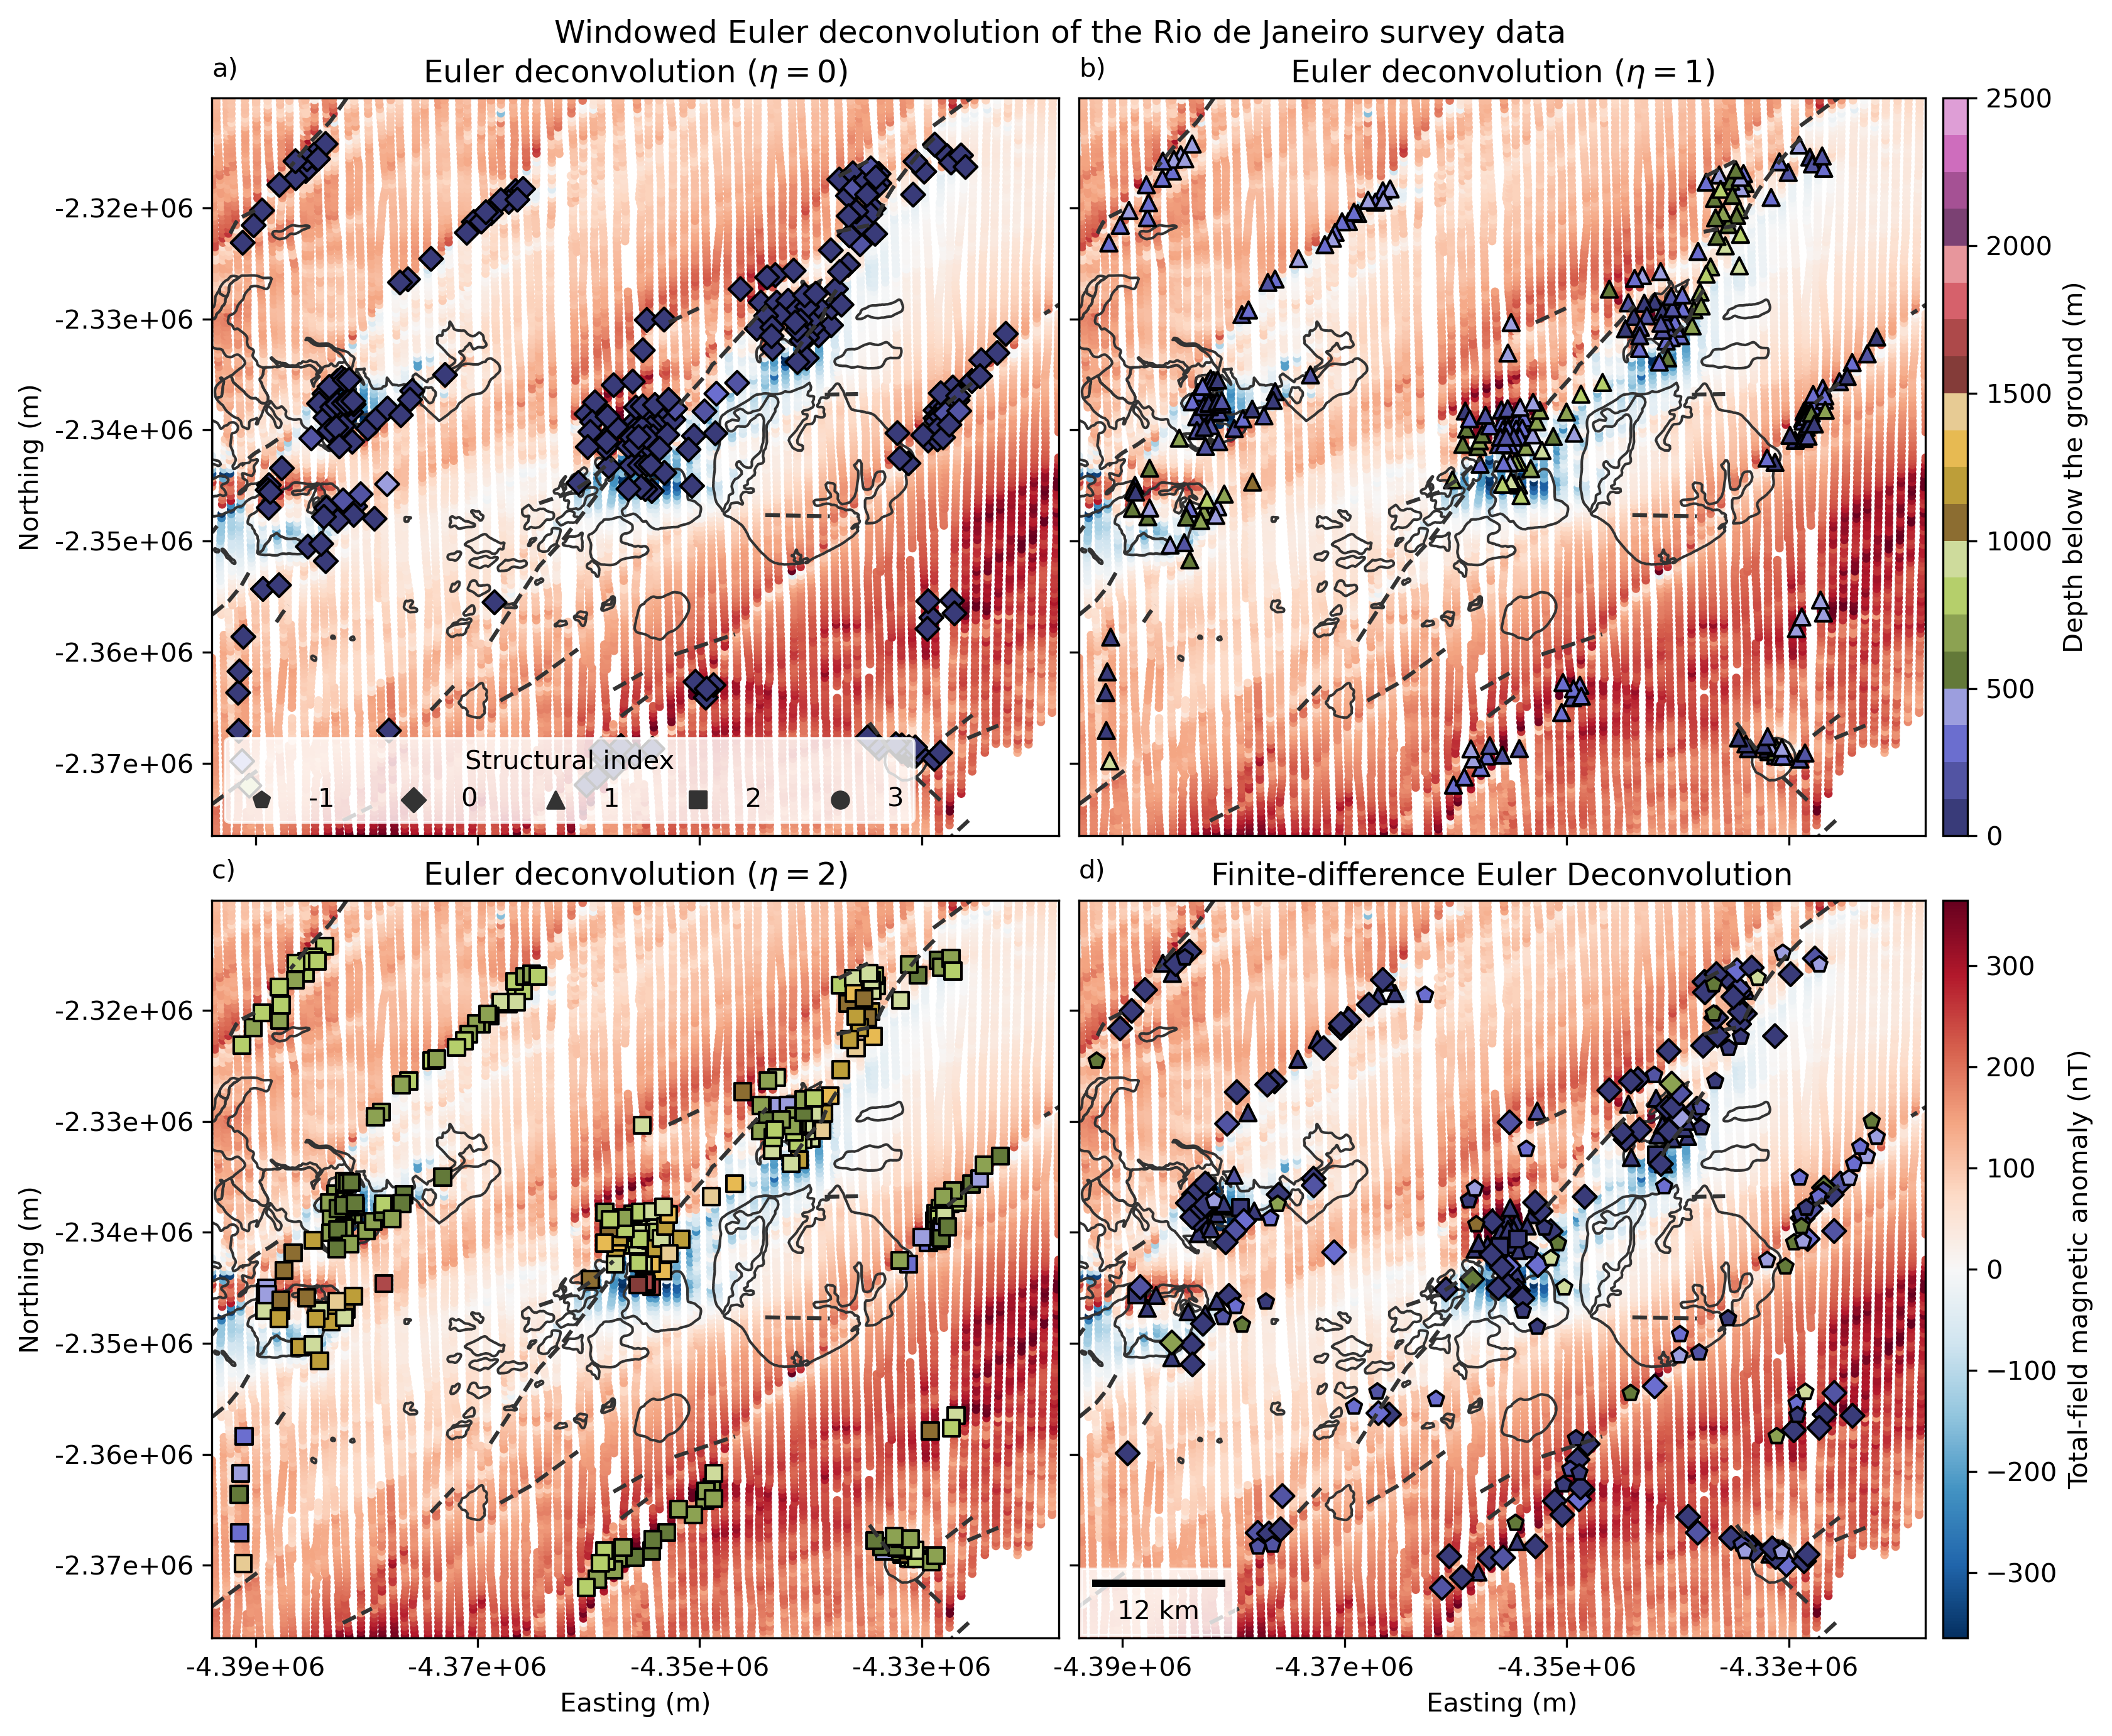
\includegraphics[width=1\linewidth]{euler-inversion/figures/real-data-application-comparison.png}
\caption{
    Results of applying Euler deconvolution and finite-difference Euler
    deconvolution with a window size of \RioWindowSize{} and a window step of
    \RioWindowStep{} to the aeromagnetic data from Rio de Janeiro, Brazil.
    a-c) Euler deconvolution results with structural index $\eta=1$, $\eta=2$,
    and $\eta=3$, respectively.
    d) Finite-difference Euler deconvolution results.
    The structural index of the solutions are represented by pentagons
    ($\eta=-1$),  diamonds ($\eta=0$),  triangles ($\eta=1$),  squares
    ($\eta=2$), and circles ($\eta=3$).
    For finite-difference Euler deconvolution, the structural index symbol is
    that of the closest integer to the estimated value.
    The colour of each symbol represents the estimated depth below the surface
    of the Earth (topography).
    Also shown are the total-field anomaly flight-line data, the contours of
    the post-collisional magmatism and alkaline intrusions (solid black lines)
    and dykes (dashed lines).
}
\label{fig:rio_comp}
\end{figure}

The geology of Rio de Janeiro state (Southeastern Brazil) consists primarily of
high-grade metamorphic rocks and granitoid magmatism related to the Ribeira
Belt (RB) \citep{Heilbron2020}.
Figure~\ref{fig:rio_context}a shows a simplified geologic map of the area,
which was modified from \citet{Heilbron2016} and \citet{Dantas2017}.
The Ribeira Belt is traditionally interpreted as a thrust
belt formed by diachronous collisions mainly between the São Francisco and
Congo paleocontinents \citep{Heilbron2008, Trouw2000} or by an intracontinental
orogeny \citep[\textit{e.g.}][]{Meira2015, Meira2019}, during the Brasiliano
orogeny. This process culminated in an orogen-parallel, steep strike-slip shear
system \citep{EgydioSilva2005}, which deformed the Paleoproterozoic basement
rocks and reworked the Meso- to Neoproterozoic metasedimentary units (for
example, the Italva and São Fidelis groups) and syn-orogenic granitoid plutons
(for example, the Rio Negro complex) which formed during the orogeny
\citep{Heilbron2003, Heilbron2020}.
These tectonic events imprinted a distinct NE-ENE-trending structural pattern
onto these rocks.

The late Neoproterozoic to Cambrian period witnessed post-orogenic magmatism
\citep[\textit{e.g.,}][]{Valeriano2011}, marking the final stages of the West
Gondwana amalgamation. After this, the region remained tectonically quiescent
until the Lower Cretaceous, when reactivation occurred with the emplacement of
the NE-trending Serra do Mar mafic dyke swarm, preceding the break-up of West
Gondwana and the opening of the South Atlantic Ocean \citep{Almeida2013}.
Lastly, thermal anomalies in the region during the Upper Cretaceous to
Paleocene period led to the emplacement of alkaline complexes and dykes
\citep{Thompson1998}.
The geological complexity of the Ribeira Belt, marked by the interplay of
diverse tectonic regimes and magmatic events (Figure~\ref{fig:rio_context}a),
makes the Rio de Janeiro region an ideal test case for Euler inversion.

We used aeromagnetic data from the state of Rio de Janeiro which are
distributed by the Serviço Geológico do Brasil
(\url{https://geosgb.sgb.gov.br}). The data were collected in two phases:
Subarea 1 was surveyed between March 25 and May 27, 1978, using an Islander
aircraft (PT-KRP), while Subarea 2 was surveyed between April 6 and
July 19, 1978, using a Bandeirante aircraft (PT-GKJ), both funded by the
Brazilian government. As shown in Figure~\ref{fig:rio_context}b, the survey
followed a pattern of north-south flight lines spaced approximately
\qty{1}{\km} apart, with east-west tie lines.
Data were recorded at 100-meter intervals using a Geometrics G-803
magnetometer. Some of the notable features of the data are the NE-SW linear
features (interpreted here as dykes), which coincide with known dyke outcrops,
and complex dipolar anomalies which coincide with some of the post-collisional
magmatism and alkaline intrusions. A subset of \RioNData{} data points were
used in our analysis.

The data were not interpolated on a regular grid to avoid any smoothing effects
that the interpolation might have on the linear features. This could result in
an over-estimation of their depth, as discussed in Section~\ref{sec:windows}.
Instead, we used the gradient-boosted equivalent sources method of
\citet{Soler2021} to fit a model to the observed line data.
We then used the model to make predictions of the three spatial derivatives at
the original measurement locations by a central-difference method with
a coordinate shift of \RioDerivSpacing{}. Further details about the data
processing can be found in the source code archive that accompanies this
article \url{https://doi.org/\ArchiveDOI} \citep{figshare}.

We performed the moving-window Euler inversion (Algorithm~\ref{alg:window} and
Algorithm~\ref{alg:si} with $\eta_{min}=\RioSIMin$ and
$\eta_{max}=\RioSIMax$) on the observed total-field anomaly line data using
windows of size of \RioWindowSize{} which were moved \RioWindowStep{} at
a time.
The proportion of solutions kept was $\gamma=0.15$.
The inversion was performed with data weights of \RioWeightsF{} for the
total-field anomaly, \RioWeightsE{} for the eastward derivative, \RioWeightsN{}
for the northward derivative, and \RioWeightsU{} for the upward derivative.
To aid in the geological interpretation of the results, we converted the
estimated upward source coordinates $z_o$ to depths below the surface of the
Earth. We did so by subtracting the estimated $z_o$ from the interpolated
topographic height of the Shuttle Radar Topography Mission
\citep[SRTM;][]{SRTM}. The estimated positions and structural indices are shown
in Figure~\ref{fig:rio_results}.
We also performed Euler deconvolution with structural indices one, two, and
three, as well as finite-difference Euler deconvolution on the same dataset
using the same window size and window step for the sake of consistency.
These results are shown in Figure~\ref{fig:rio_comp}.

The Euler inversion estimated source positions shown in
Figure~\ref{fig:rio_results} highlight the NE-SW lineaments as well as some of
the more dipolar anomalies.
The lineaments are estimated with a mix of $\eta=1$, $\eta=2$, and $\eta=3$.
The southernmost lineament is mostly estimated with $\eta=1$ and depths
suggesting that it does not outcrop in its southernmost parts (depths of
\qtyrange{400}{600}{\m}), which is consistent with the geologic information in
Figure~\ref{fig:rio_context}a. The southernmost part of this lineament, in
particular, has an estimated $\eta=3$, which is known to happen for deeper
dykes in our synthetic data tests (Section~\ref{sec:windows}). Conversely, the
northernmost part of the lineament has a larger prevalence of $\eta=1$ with
shallower depths which coincide with a known dyke outcrop.
Other known dyke outcrops coincide with estimated sources with $\eta=1$,
however their depths range from \qtyrange{100}{300}{\m}. This may be caused by
an excess of smoothing in the vertical derivative or effects of noise in the
estimated coordinates. The lineaments in the northwestern part of the region
are also highlighted by estimated sources.
However, their structural indices are a mix of $\eta=2$ and $\eta=3$,
suggesting deeper sources. This is inline with the geologic information, which
includes no outcrops of linear structures in the area.

The dipolar anomalies are associated with post-collisional and alkaline
intrusions, many of which are also cut by known outcropping dykes or have known
dykes with magnetic signals that significantly overlap with the dipolar
anomalies. The Euler inversion estimated structural indices for them range from
$\eta=2$ to $\eta=3$. We have highlighted four dipolar anomalies, marked as A,
B, C, and D in Figure~\ref{fig:rio_results}, to aid in our discussion.

\begin{itemize}
\item \textbf{Anomaly A:} Has a reversed polarity and linear feature to its
    north that is not associated with any known dyke outcrop. The linear
    feature is highlighted by Euler inversion estimates with $\eta=1$ and depth
    of \qtyrange{300}{400}{\m}, which can be interpreted as a non-outcropping
    dyke. The dipolar anomaly itself has Euler inversion solutions with
    $\eta=3$ and depth of \qtyrange{1000}{2000}{\m}.
    The solutions in the centre of the anomaly present a shallower depth than
    the solutions to the north and south of the anomaly centre. From the
    results on synthetic data in Section~\ref{sec:windows}, we can interpret
    the depth range to be caused by the moving window procedure and the effect
    of interfering sources. The depth to the centre of the anomaly source is
    likely close to \qty{1000}{\m}.

\item \textbf{Anomaly B:} The dipolar anomaly is likely associated with
    a non-outcropping portion of the post-collisional magmatism. The anomaly is
    cut by several NE-SW linear features, some of which overlap with known dyke
    outcrops. The linear feature to the north is associated with Euler
    inversion results with $\eta=1$ and depths ranging from
    \qtyrange{300}{600}{\m}, suggesting a non-outcropping dyke. At the centre
    of the anomaly are Euler inversion estimates with $\eta=3$ and depth
    estimate of approximately \qty{1400}{\m}. The Euler inversion solutions
    surrounding these central solutions are likely caused by interference from
    other sources.

\item \textbf{Anomaly C:} A dipolar anomaly associated with an outcropping
    portion of the post-collisional magmatism. There is a known outcropping
    dyke to the south of the anomaly, which is associated with Euler inversion
    estimates with $\eta=1$ and depths ranging from \qtyrange{500}{1000}{\m}.
    These depth estimates are likely overestimated because of the interference
    of the dipolar anomaly. The main anomaly has Euler inversion solutions with
    $\eta=2$ and $\eta=3$ and depths varying from \qtyrange{1400}{1800}{\m}.
    There is no clear indication of which of these estimates is more reliable.

\item \textbf{Anomaly D:} A small dipolar anomaly associated with an
    outcropping alkaline intrusion. The Euler inversion estimates have $\eta=3$
    and depths \qtyrange{1700}{2000}{\m}. There are known outcropping dykes
    around the main intrusion but they have no discernible magnetic anomalies
    and no Euler inversion solutions associated with them.
\end{itemize}

Overall, the Euler inversion solutions in Figure~\ref{fig:rio_results} are
consistent with the known geology in Figure~\ref{fig:rio_context}a.
The main linear features are mostly associated with Euler inversion estimates
with $\eta=1$ and shallow depths, particularly where known dyke outcrops are
located.
Deeper linear features are estimated with $\eta=2$ and $\eta=3$, which is
consistent with the synthetic data results (Section~\ref{sec:windows}).
The dipolar anomalies have consistent Euler inversion estimates with $\eta=3$
when they are well isolated from interfering sources.
Otherwise, they are estimated with a mix of structural indices and depths, as
was demonstrated in Section~\ref{sec:windows}.

When compared to the Euler deconvolution and finite-difference Euler
deconvolution results (Figure~\ref{fig:rio_comp}), the Euler inversion results
are less dispersed and better delinear the linear features present in the data.
The structural index results from finite-difference Euler deconvolution
(Figure~\ref{fig:rio_comp}d) are underestimated, with most values of $\eta$
being less than one, which is not in accordance with the geology of the area.

%%%%%%%%%%%%%%%%%%%%%%%%%%%%%%%%%%%%%%%%%%%%%%%%%%%%%%%%%%%%%%%%%%%%%%%%%%%%%%%
\section{Conclusion}

Euler deconvolution is a widely used method for locating the sources of
potential-field data.
It has its limitations in real-world scenarios due to its dependence on the
chosen value of the structural index $\eta$ and its sensitivity to
high-frequency noise and signal overlap from interfering sources.
We have developed a new method to solve Euler's homogeneity equation for the
source position, base level, and integer structural index, which we call
\textit{Euler inversion}.
Unlike Euler deconvolution, Euler inversion is also able to estimate the
predicted field and its spatial derivatives, as well as assign different
weights to each type of data.
Our method can be applied to gridded and non-gridded data, which can
be useful to limit the effects of smoothing from interpolation in the final
results when the original data have large spacing between flight lines.
The Euler inversion algorithm is computationally efficient because most of the
large matrices involved in the computations are diagonal or block-diagonal.
We found that, in practice, the computation time of Euler inversion and Euler
deconvolution are on the same order of magnitude.

Tests on synthetic data show that Euler inversion outperforms Euler
deconvolution and finite-dif\-fer\-ence Euler deconvolution (a variant that
estimates $\eta$ but does not rely on second-order derivatives) in terms of
robustness to random noise and interfering sources inside the data window.
Our tests also show that the estimated $z_o$ coordinate is correlated with the
structural index, as is the case for Euler deconvolution.
We have also found that the data misfit from Euler inversion is minimal when
the integer structural index used is equal or close to the true one for
idealized sources.
This led us to develop an algorithm for estimating the best integer structural
index based on the data misfit.
A test on complex synthetic data from a model of dykes and dipoles with
overlapping signals shows that Euler inversion is able to estimate the
structural index and position of the sources within expected error bounds when
the signal overlap is not larger than the data window.
For deeper dykes in particular, Euler inversion was not able to estimate the
correct $\eta=1$, leading to an overestimation of the depths.

We applied Euler inversion to an aeromagnetic dataset from Rio de Janeiro,
Brazil, to analyse its performance under real-world scenarios.
Euler inversion was able to locate the NE-SW linear features in the data with
an $\eta=1$ which are associated with known dyke outcrops.
For the deeper linear features, Euler inversion was not able to estimate the
correct $\eta=1$.
Some of the dipolar anomalies present in the data were picked out with
$\eta=3$, while the sources with a large signal overlap with other features
provided a mix of $\eta=2$ and $\eta=3$.
These results are consistent with the synthetic data tests and show the
benefits and limitations of the proposed method.

Euler inversion outperforms Euler deconvolution and finite-difference Euler
deconvolution in most cases.
Its reduced sensitivity to noise and interfering sources, in particular,
may prove beneficial for magnetic microscopy studies, in which high-frequency
noise and interference from multiple dipolar sources are a significant hurdle
\citep{SouzaJunior2024}.
However, it still suffers from some of the same limitations.
While Euler inversion is less sensitive to signal overlap, it still fails to
correctly estimate the position and structural index when the overlap is large.
The windowing procedure still generates a large amount of spurious solutions
which need to be filtered out.
This could be improved with techniques like the source detection method
proposed by \citet{Castro2020}, for example.
Euler inversion can also be coupled with other inverse problems by following
our methodology to add Euler's equation as a non-linear constraint.
This could help with issues of non-uniqueness and stability in traditional 3D
inverse problems in potential-field methods.

As is the case with other Euler deconvolution-based methods, Euler inversion
also suffers from instability when sources are 2D \citep{Mushayandebvu2004}
and a lack of support for sources that are defined by multiple points, for
example steps which have a top and bottom \citep{Gerovska2010}.
The issue of instability was evident in our synthetic data tests which
simulated dykes and did not contaminate the data with random noise.
However, both in the synthetic data tests with noise and the real data
application, this did not appear to be a significant issue.
In both cases, Euler inversion was better at outlining the 2D sources than
Euler deconvolution.
Nonetheless, it would be worthwhile to investigate this issue further and
explore the use of regularization and an adaptation of the method of
\citet{Mushayandebvu2004} to the Euler inversion mathematical formulation.
A thorough comparison of Euler inversion with the Similarity Transform-based
methods, like \citet{Gerovska2010}, would also be worth pursuing.
Euler inversion could complement such methods, which often require gridded
data, in cases where data are of poor quality or flight-line spacing is large.


%%%%%%%%%%%%%%%%%%%%%%%%%%%%%%%%%%%%%%%%%%%%%%%%%%%%%%%%%%%%%%%%%%%%%%%%%%%%%%%
\section*{Data availability statement}

The Python source code and data that were used to produce all results and
figures presented here are available at
\url{https://github.com/\GitHubRepository}
and \url{https://doi.org/\ArchiveDOI} \citep{figshare}
under the CC-BY license and the MIT license.
This study made use of the following open-source scientific software:
matplotlib \citep{matplotlib} and PyGMT \citep{pygmt} for generating figures
and maps,
Numpy \citep{numpy} and Scipy \citep{scipy} for linear algebra,
Pandas for manipulating tabular data \citep{McKinney2010,pandas},
GeoPandas for reading and plotting shapefiles \citep{geopandas},
pyproj for data projection \citep{pyproj},
xarray \citep{xarray} for working with gridded data,
Verde \citep{verde} for moving windows and interpolation,
and Harmonica \citep{harmonica} for potential-field data processing and
modeling.
The aeromagnetic and geologic data are available from Serviço Geológico do
Brasil (\url{https://geosgb.sgb.gov.br}) under a CC-BY-NC license.
The magnetic data are part of survey 1038 ``Projeto Aerogeofísico São Paulo --
Rio de Janeiro''.
Both are also available in our source code and data archive \citep{figshare}.


%%%%%%%%%%%%%%%%%%%%%%%%%%%%%%%%%%%%%%%%%%%%%%%%%%%%%%%%%%%%%%%%%%%%%%%%%%%%%%%
\section*{Acknowledgements}

We are indebted to the developers and maintainers of the open-source software
without which this work would not have been possible.
We thank Dr. Valéria C. F. Barbosa for many insightful discussions over the
years which helped shape our research.
We are grateful to editor Dr. Kosuke Heki and reviewers Dr. Alan B. Reid and
Dr. Saulo Oliveira for their constructive comments.
LU would like to thank Prof. Spiros Pagiatakis for being an incredible
instructor and teaching him the mathematics which formed the foundations of
this work during his undergraduate exchange at York University.
LU was supported in part by start-up grant PRPI 22.1.09345.01.2 from
Universidade de São Paulo.
GFSJ was supported by scholarship 2021/08379-5 from the Fundação de Amparo
à Pesquisa do Estado de São Paulo (FAPESP).
The opinions, hypotheses, and conclusions or recommendations expressed in this
material are the responsibility of the authors and do not necessarily reflect
the views of FAPESP.

\section*{CRediT author contributions}

\textbf{Leonardo Uieda:} Conceptualisation, Data curation, Formal analysis,
Investigation, Methodology, Pro\-ject administration, Resources, Software,
Supervision, Visualisation, Writing – original draft.

\noindent
\textbf{Gelson Ferreira Souza-Junior:} Data curation, Formal analysis,
Resources, Software, Visualisation, Writing - original draft, Writing - review
\& editing.

\noindent
\textbf{India Uppal:} Data curation, Formal analysis, Investigation, Software,
Writing - review \& editing.

\noindent
\textbf{Vanderlei Coelho Oliveira Jr.:} Conceptualisation, Methodology, Writing
- review \& editing.

\endgroup

%==============================================================================
% \bookmarksetup{startatroot}
\chapter{Conclusion}

Bla.


%%%%%%%%%%%%%%%%%%%%%%%%%%%%%%%%%%%%%%%%%%%%%%%%%%%%%%%%%%%%%%%%%%%%%%%%%%%%%%%
\bibliographystyle{apalike-doi}
\bibliography{references}

\end{document}
